\documentclass[a5paper,DIV=12,BCOR=9mm,headsepline,headings=small,cleardoubleempty,10pt,hyperref,UTF8]{scrbook}
\usepackage{scrpage2}
\usepackage{Open-Advice}
\usepackage[utf8]{inputenc}
\usepackage{textcomp}
\usepackage{graphicx}
\usepackage{xcolor}
\usepackage{tabularx}
\usepackage{indentfirst}
%\usepackage[english]{babel}

\usepackage[CJKspace]{xeCJK}

\setCJKmainfont
    [
      BoldFont   = WenQuanYi Micro Hei,
      ItalicFont = AR PL KaitiM GB,
    ]
    {AR PL SungtiL GB}
\setCJKsansfont{WenQuanYi Zen Hei}
\setCJKmonofont{WenQuanYi Micro Hei Mono}


\usepackage[raiselinks=true,
bookmarks=true,
bookmarksopenlevel=1,
bookmarksopen=true,
bookmarksnumbered=true,
hyperindex=true,
plainpages=false,
pdfpagelabels=true,
pdfborder={0 0 0.5}
]{hyperref}


% Meta data
\newcommand{\booktitle}{开源建议书Open Advice}
\newcommand{\booksubtitle}{自由开源软件: 投入之后我们才知道的那些事}
\newcommand{\bookeditor}{Lydia Pintscher}
\newcommand{\bookyear}{2012}
\newcommand{\bookisbn}{978-1-105-51493-7}
\newcommand{\bookurl}{http://open-advice.org}
\newcommand{\bookauthors}{Georg Greve, Armijn Hemel, Evan Prodromou, Markus Krötzsch, Felipe Ortega, Leslie Hawthorn, Kévin Ottens, Lydia Pintscher, Jeff Mitchell, Austin Appel, Thiago Macieira, Henri Bergius, Kai Blin, Ara Pulido, Andre Klapper, Jonathan Leto, Atul Jha, Rich Bowen, Anne Gentle, Shaun McCance, Runa Bhattacharjee, Guillaume Paumier, Federico Mena Quintero, Máirín Duffy Strode, Eugene Trounev, Robert Kaye, Jono Bacon, Alexandra Leisse, Jonathan Riddell, Thom May, Vincent Untz, Stuart Jarvis, Jos Poortvliet, Sally Khudairi, Nóirín Plunkett, Dave Neary, Gareth J. Greenaway, Selena Deckelmann, Till Adam, Frank Karlitschek, Carlo Daffara, Dr. Till Jaeger, Shane Coughlan}

\hypersetup{
  pdfauthor={\bookauthors},
  pdftitle={\booktitle},
  pdfsubject={Open Source, Free Software},
  pdfkeywords={Open Source, Free Software},
  pdflang=zh,
  colorlinks,
  linkcolor=black,
  anchorcolor=black,
  filecolor=black,
  urlcolor=black,
  citecolor=black,
  bookmarksnumbered=true,
  pdfpagelayout=TwoColumnRight
}
\ifusinght
\else
  \usepackage{xmpincl}
  %  \includexmp{Open-Advice}
  \usepackage{pdfpages}
\fi
\hyphenation{pro-ject pro-jects Free-desk-top Wiki-pe-dia fund-rais-ing pro-spec-tus-es pro-vi-ders}

\pagestyle{scrheadings}
\ihead[]{\headmark}
\ohead[]{\pagemark}
%\cfoot[]{Open Advise}
\ifoot[]{ }
\ofoot[]{ }

% Use a nicer-Looking design for the TOC
\usepackage{tocstyle}
\usetocstyle{KOMAlike}

% Avoid typographical unpleasantries
\clubpenalty = 10000
\widowpenalty = 10000
\displaywidowpenalty = 10000
% Avoids line-overshooting at the cost of "Word-like" spacing
\setlength{\emergencystretch}{0.25em}
\settowidth{\parindent}{2em}
\begin{document}

\ifusinght
\else
  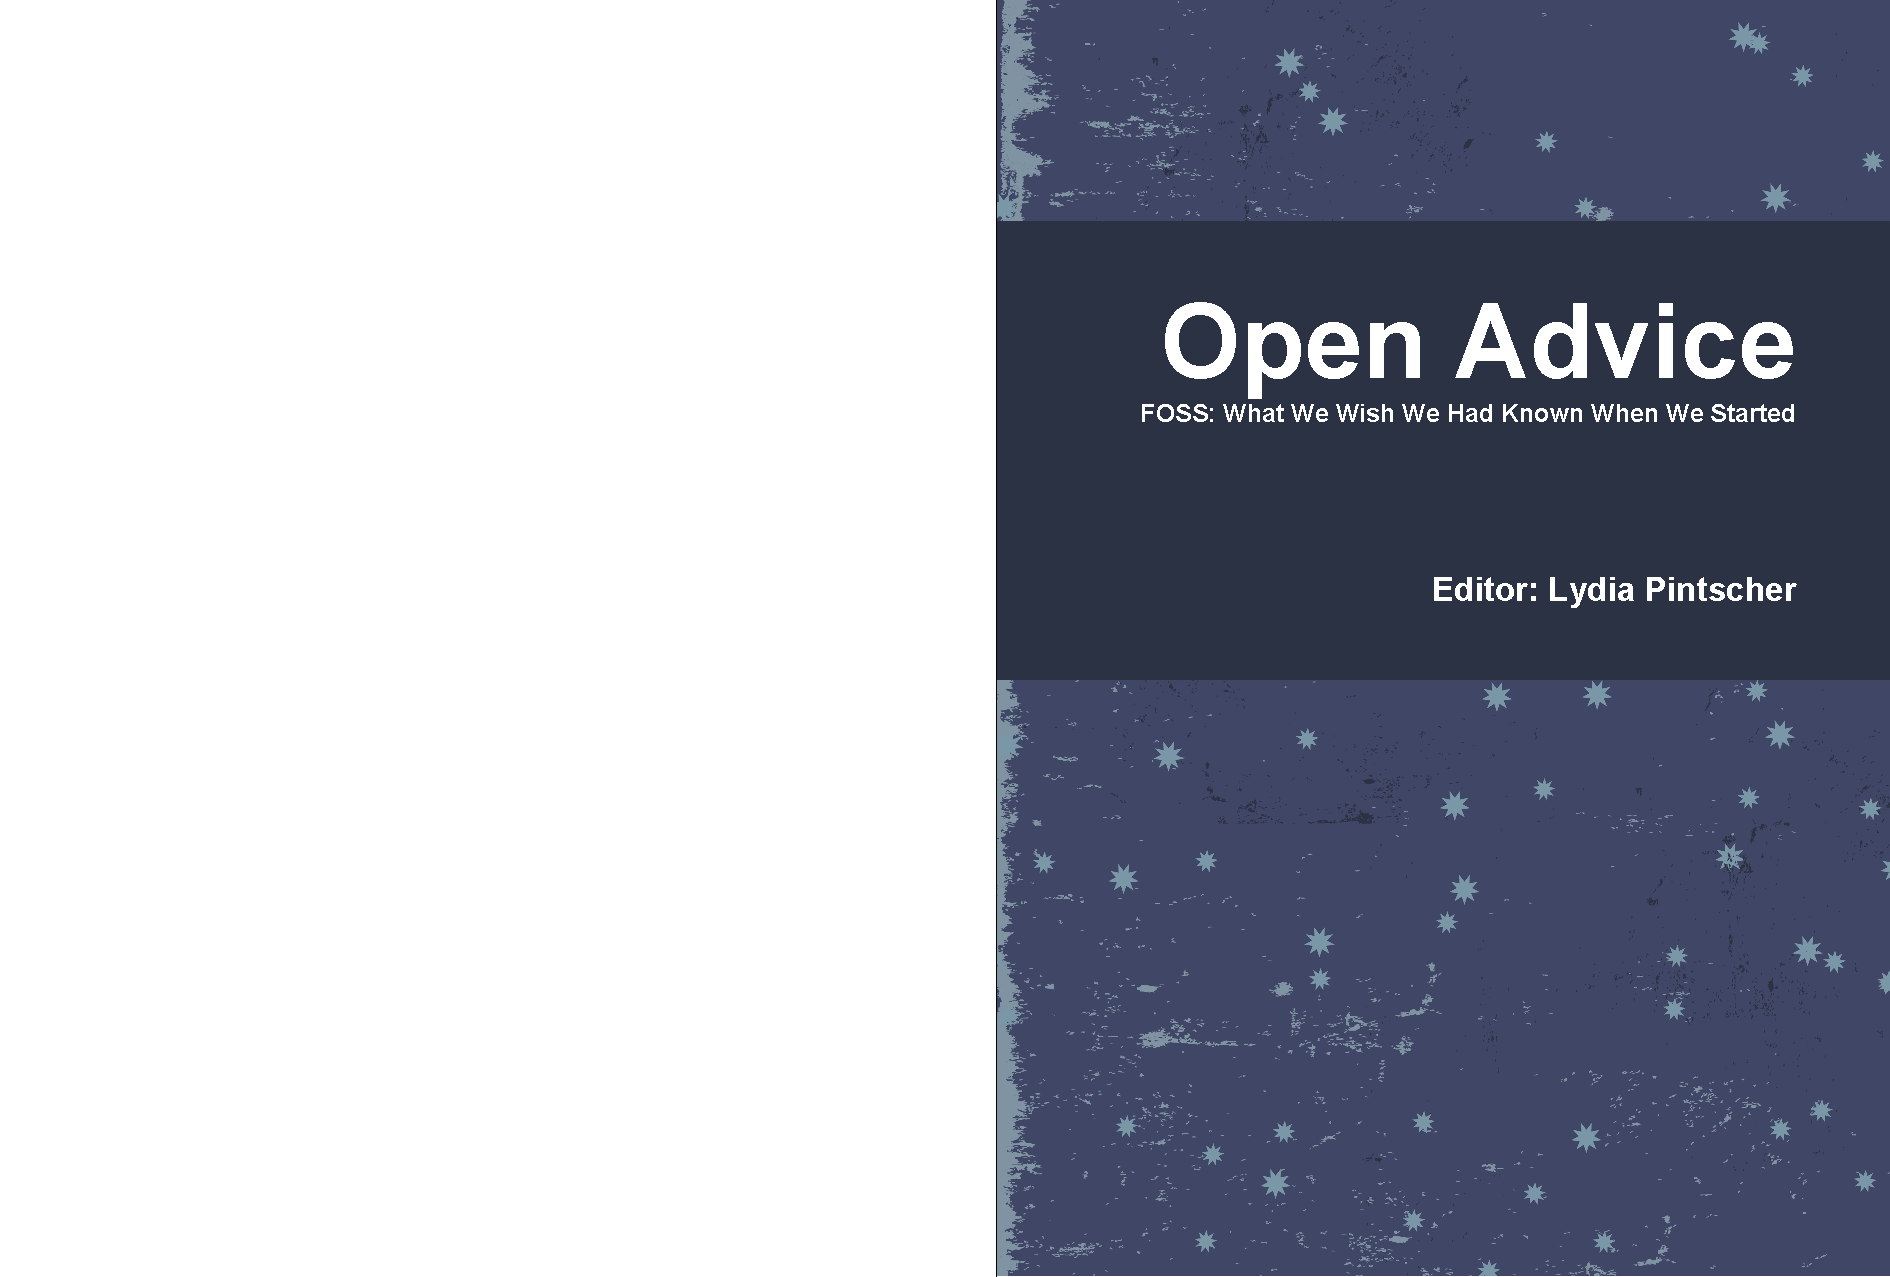
\includepdf[noautoscale]{frontcover}
\fi
\frontmatter
\thispagestyle{empty}
% Extra title page
\booktitle
\newpage
% empty page back
\newpage
% inner title page
\begin{titlepage}
\begin{flushright}
\bookeditor{} (Editor)\\
\vspace{10em}
{\Huge\bfseries\sffamily\booktitle}\\
\vspace{2em}
{\large\sffamily\booksubtitle}
\end{flushright}
\end{titlepage}
% titleback
\thispagestyle{empty}
拉萨的会计法塑料袋会计分录看拉萨的看风景阿隆索的就拉萨的分开了撒旦狂风巨浪萨克达发jThe information in this book is distributed on an ``As Is'' basis, without warranty. While every precaution has been taken in the preparation of this work, neither the authors nor the editor or publishers shall have any liability to any person or entity with respect to any loss or damage caused or alledged to be caused directly or indirectly by the information contained in it.%
\vfill
Copyright \textcopyright{} \bookyear{} \bookauthors\\
\newline
\fbox{\parbox{\textwidth}{
\begin{center}
\includegraphics{cc-by-sa.png}\end{center}
This work is licensed under a Creative Commons Attribution-ShareAlike 3.0 License. To view a copy of this license visit: \\{\small\url{http://creativecommons.org/licenses/by-sa/3.0/legalcode}}.
\vspace{0.25em}
}}
\newline \\
Visit \url{http://www.open-advice.org} to download this book as PDF or eBook and receive additional information.
\newline \\
{\tt ISBN: \bookisbn}%
%dedication
\newpage
\thispagestyle{empty}
\vspace*{2cm}
\begin{flushright}
{\Large\itshape for giants\\and those who will stand on their shoulders}\\
\end{flushright}
\newpage
\thispagestyle{empty}
\mbox{}
\newpage
%End of top matter

\section*{前言}


此书是一本有关社区与技术相关的书籍。这本书体现了众多人合作的价值,正如我们合力所构建的技术。事实上,如果你第一次参与到社区中来,你会感到奇怪:社区的背后竟然是以技术来驱动的。难道没有大型技术公司参与么?事实上,对我们来说这几乎是不存在的。

This is a book about community and technology. It is a book that
represents a collective effort, much like the technology we build
together. And if this is in fact your first encounter with our
community, you may find it strange to think of a community as the
driving force behind technology. Isn't technology built by large
corporations? Actually, for us it is almost the other way around.


The authors in this book are all members of what you could label the
software freedom community. A group of people sharing the fundamental
experience that software is more empowering, more useful, more
flexible, more controllable, more just, more encompassing, more
sustainable, more efficient, more secure and ultimately just better
when it comes with four fundamental freedoms: to use, study, share and
improve the software.

And while there is now an increasing number of communities that have left
behind the requirement for geographical proximity by means of virtual
communication, it was this community that pioneered that new age. 

In fact, the Internet and the Free Software Community\footnote{For me,
  Open Source is one aspect of that community. This particular aspect
  articulated itself in 1998, so quite some time after the Internet
  came about. But please feel free to replace Free Software by Open
  Source in your head if that is your preferred terminology.}  were
co-dependent developments. As the Internet grew, our community could
grow with it, but without the values and technology of our community,
I have no doubts that the Internet would not have become the
all-encompassing network that we now see enabling people and groups
around the world.

Until today, our software runs most of the Internet, and you will know
at least some of it, such as Mozilla Firefox,
OpenOffice.org, Linux, and perhaps even GNOME or KDE. But our
technology may also be hidden inside your TV, your wireless
router, your ATM, even your radio, security system or battleships. It
is literally everywhere. 

It was essential in enabling some of the large corporations
that you know, such as Google, Facebook, Twitter and others. None of
these could have achieved so much in such a short time if it were not
for the power of software freedom that allowed them to stand on the
shoulders of those who came before.

But there are many smaller companies that live from, with, and for
Free Software, including my own, Kolab Systems. Active partaking in
the community in good faith and standing has become a critical success
factor for all of us. And this is true even for the large ones, as
Oracle has involuntarily demonstrated during and after its takeover of
Sun Microsystems.

But it is important to understand that our community is \textbf{not}
anti-commercial. We enjoy our work, and many of us have made it their
profession for their livelihood and mortgage. So when we say
community, we mean students, entrepreneurs, developers, artists,
documentation writers, teachers, tinkerers, businessmen, sales people,
volunteers and users.

Yes, users. Even if you did not realize it or ``never signed up for no
community,'' you in fact are already \emph{almost} part of ours. The
question is whether you'll choose to participate actively.

And this is what sets us apart from the monoculture behemoths, the
gated communities, the corporate owned walled gardens of companies
like Apple, Microsoft and others. Our doors are open. So is our
advice. And your potential. There is no limit as to what you can
become -- it purely depends on your personal choice as it has
depended for each of us.

So if you are not yet part of our community, or simply curious, this
book provides a good starting point. And if you are already an active
participant, this book might provide you with insights into a few
facets and perspectives that are new to you.

Because this book contains important grains of that implicit
knowledge which we usually build and transfer inside our
sub-communities that work on different technologies. This knowledge
typically trickles down from experienced contributors to less
experienced ones, which is why it seems very obvious and
natural to those socialized in our community.

This knowledge and culture of how to shape collaboration allows us to
build outstanding technology in small, distributed teams across
language, country and cultural barriers around the world,
outperforming much larger development teams in some of the world's
largest corporations.

All the people writing in this book are such experienced contributors
in one, sometimes several areas. They have grown to become teachers
and mentors. Over the course of the past 15 years or so I had the
pleasure of getting to know most of them, working with many, and the
privilege to call some of them friends. 

Because as Kévin Ottens rightly said during the Desktop Summit 2011 in
Berlin: ``Community building is family and friendship building.''

So it is in fact with a profound sense of gratitude that I can say
there is no other community I would rather be part of, and I look
forward to hopefully seeing you at one or the other upcoming
conference.
\newline
\begin{flushright}--- Georg Greve\end{flushright}
\begin{flushright}Zürich, Switzerland; 20. August 2011\end{flushright}

\textit{Georg Greve initiated the Free Software Foundation Europe in
2000 and was its founding president until 2009. During this time he
was responsible for building up and designing many of FSFE's activities
such as the Fellowship, the policy or legal work, and has worked
intensively with many communities. Today he continues this work as
shareholder and CEO of Kolab Systems AG, a fully Free Software company.
For his accomplishments in Free Software and Open Standards Georg
Greve was awarded the Federal Cross of Merit on ribbon by the Federal
Republic of Germany on 18 December 2009.}

\newpage

\section*{Thank You!}

This book would not have been possible without the support of each of the
authors and the following people, who helped make it happen:
\begin{itemize}
 \item Anne Gentle (editing)
 \item Bernhard Reiter (editing)
 \item Celeste Lyn Paul (editing)
 \item Daniel Molkentin (layout)
 \item Debajyoti Datta (website)
 \item Irina Rempt (editing)
 \item Jeff Mitchell (editing)
 \item Mans Rullgard (editing)
 \item Noirin Plunkett (editing)
 \item Oregon State University Open Source Lab (website hosting)
 \item Stuart Jarvis (editing)
 \item Supreet Pal Singh (website)
 \item Saransh Sinha (website)
 \item Vivek Prakash (editing)
 \item Will Kahn-Greene (editing)
\end{itemize}

\newpage

\tableofcontents
\mainmatter
\part{启迪与创新}
\chapterwithauthor{Armijn Hemel}{先写代码}

\authorbio{Armijn Hemel has been using free software since 1994, when his brother
came home with a stack of floppies with an early version of FreeBSD. A year
later the switch to Linux was made and he has been using Unix(-like) systems
ever since then, both at home, during his studies at Utrecht University and at
work.
Since 2005, Armijn has been part of the core team of gpl-violations.org and
has his own consultancy (Tjaldur Software Governance Solutions) specialized
in detection and resolution of GPL license violations.}

\noindent{}Back in 1999 I was just getting started in FLOSS activism. I had already
been using Linux and FreeBSD for a number of years then, but I was merely a user and
I wanted to actually contribute something back. The best way I thought for
contributing back was to write code. I could not find any existing project I
would be comfortable working on, so I decided to start my own project. In
hindsight the reason why I did that was probably a mixture of various things.
One factor was insecurity whether or not my code was actually good enough to be
accepted in an existing project (I was, and still am, no brilliant programmer)
and with your own project that is not much of an issue. The second reason is
probably youthful arrogance.

My idea was to make a presentation program, which would fancy more of the
advanced (or, annoying, if you wish) features of PowerPoint. Back in that time
there was no OpenOffice.org and choices were pretty limited to LaTeX and
Magicpoint, which are more tailored to delivering text content, than to showing
whirly effects. I wanted to make the program cross platform and back then I
thought Java would be the best choice for this. The idea was to make a
presentation program, written in Java, which would have support for all those
whirly effects. I made up my mind and started the project.

Infrastructure-wise everything was there: there was a mailing list, there was a
website, there was source code control (CVS). But there was no actual code for
people to work on. The only things I had were some ideas of what I wanted to do,
an itch to scratch and the right buzzwords. I actually wanted people to join in
creating this program and make it a truly collaborative project.

I started making designs (with some newly acquired UML knowledge) and sent them
around. Nothing happened. I tried to get people involved, but collaboratively
working on a design is very hard (besides, it is probably not the best way to
create software in the first place). After a while I gave up and the project
silently died, without ever producing a single line of code. Every month I was
reminded by the mailing list software that the project once existed, so I asked
it to be taken offline.

I learned a very valuable, but somewhat painful, lesson: when you announce
something and when you want people to get involved in your project, at least
make sure there is some code available. It does not have to be all finished, it
is OK if it is rough (in the beginning that is), but at least show that there is
a basis for people to work with and improve upon. Otherwise your project will go
where many many projects, including my own failed project, have gone: into
oblivion.

I eventually found my niche to help advance FLOSS, by making sure that the legal
underpinnings of FLOSS are tight through the gpl-violations.org project. In
retrospect I have never used, nor missed, the whirly effects in presentation
programs and found them to be increasingly irritating and distracting too much
from the content. I am happily using LaTeX beamer and occasionally (and less
happily) OpenOffice.org/LibreOffice to make presentations.

\chapterwithauthor{Evan Prodromou}{Everyone Else Might Be Wrong, But Probably Not}

\authorbio{Evan Prodromou is the founder of Wikitravel, StatusNet and the Open Source social
network Identi.ca. He has participated in Open Source software for 15 years as a
developer, documentation writer, and occasional bomb-throwing crank. He lives in
Montreal, Quebec.}

\noindent{}The most important characteristic of the Open Source project founder, in the
first weeks or months before releasing their software into the world, is
mule-headed persistence in the face of overwhelming factual evidence. If your
software is so important, why has someone else not written it already? Maybe it is not even possible. Maybe nobody else wants what you are making. Maybe you are not good enough to make it. Maybe someone else already did, and you are just not good enough at Googling to find it.

Keeping the faith through that long, dark night is hard; only the most
pig-headed, opinionated, stubborn people make it through. And we get to exercise
all our most strongly-held programmer's opinions. What is the best programming
language to use? Application architecture? Coding standards? Icon colors?
Software license? Version control system? If you are the only one who works on
(or knows about!) the project, you get to decide, unilaterally.

When you eventually launch, though, that essential characteristic of stubborn
determination and strong opinion becomes a detriment, not a benefit. Once you have launched, you will need exactly the opposite skill to make compromises to make your software more useful to other people. And a lot of those compromises will feel really wrong.

It is hard to take input from ``outsiders'' (e.g., people who are not you). First, because they focus on such trivial, unimportant things -- your variable naming convention, say, or the placement of particular buttons. And second, because they are invariably wrong -- after all, if what you have done is not the right way to do it, you would not have done it that way in the first place. If your way was not the right way, why would your code be popular?

But ``wrong'' is relative. If making a ``wrong'' choice makes your software more
accessible for end users, or for downstream developers, or for administrators or
packagers, is that not really right?

And the nature of these kind of comments and contributions is usually negative.
Community feedback is primarily reactive, which means it is primarily critical.
When was the last time you filed a bug report to say, ``I really like the
organization of the hashtable.c module.'' or ``Great job on laying out that
sub-sub-sub-menu.''? People give feedback because they do not like the way things work right now with your software. They also might not be diplomatic in
delivering that news.

It is hard to respond to this kind of feedback positively. Sometimes, we flame
posters on our development mailing lists, or close bug reports with a sneer and
a WONTFIX. Worse, we withdraw into our cocoon, ignoring outside suggestions or
feedback, cuddling up with the comfortable code that fits our preconceptions and
biases perfectly.

If your software is just for you, you can keep the codebase and surrounding
infrastructure as a personal playground. But if you want your software to be
used, to mean something to other people, to (maybe) change the world, then
you are going to need to build up a thriving, organic community of users, core
committers, admins and add-on developers. People need to feel like they own the
software, in the same way that you do.

It is hard to remember that each one of those dissenting voices is the tiny
corner of the wedge. Imagine all the people who hear about your software and
never bother to try it. Those who download it but never install it. Those who
install it, get stuck, and silently give up. And those who do want to give you
feedback, but can not find your bug-report system, developers mailing list, IRC
channel or personal email address. Given the barriers to getting a message
through, there are likely about 100 people who want to see change for
every one person to get the message through. So listening to those voices, when
they do reach you, is critical.

The project leader is responsible for maintaining the vision and purpose of the
software. We can not vacillate, swinging back and forth based on this or that
email from random users. And if there is a core principle at stake, then, of
course, it is important to hold that core steady. No one else but the project
leader can do that.

But we have to think: are there non-core issues that can make your software more
accessible or usable? Ultimately the measure of our work is in how we reach people, how our software is used, and what it is used for. How much does our personal idea about what is ``right'' really matter to the project and to the community? How much is just what the leader likes, personally? If those non-core issues exist, reduce the friction, respond to the demand, and make the changes. It is going to make the project better for everyone.


\part{Research}
\chapterwithauthor[Out of the Lab, into the Wild]{Markus Kr\"otzsch}{Out of the Lab, into the Wild: Growing Open Source Communities around Academic Projects}

\authorbio{Markus Kr\"otzsch is a post-doctoral researcher at the Department of
Computer Science of the University of Oxford. He obtained his Ph.D. from the
Institute of Applied Informatics and Formal Description Methods (AIFB) of the
Karlsruhe Institute of Technology (KIT) in 2010. His research interest is the
intelligent automatic processing of information, ranging from the foundations of
formal knowledge representation to application areas like the Semantic Web. He
is the lead developer of the successful Semantic Web application platform
Semantic MediaWiki, co-editor of the W3C OWL 2 specification, chief maintainer
of the semanticweb.org community portal, and co-author of the textbook
Foundations of Semantic Web Technologies.}

\noindent{}Academic researchers develop large amounts of software, be it for validating a
hypothesis, for illustrating a new approach, or merely as a tool to aid some
study. In most cases, a small focused prototype does the job, and it is
disposed quickly after the focus of research moves on. However, once in a while,
a novel approach or upcoming technology bears the potential to really change the
way in which a problem is solved. Doing so promises professional reputation,
commercial success, and the personal gratification of realizing the full
potential of a new idea. The researcher who made this discovery then is tempted
to go beyond a prototype towards a \emph{product} \emph{产品} that is actually used -- and
is faced by a completely new set of practical problems.

\section*{The Fear of the User}

Frederick P.\ Brooks, Jr., in one of his famous essays on software engineering,
gives a good picture of the efforts related to maintaining real software, and
warns us of the user:
%
\begin{quote}
``The total cost of maintaining a widely used program is typically 40 percent or
more of the cost of developing it. Surprisingly, this cost is strongly affected
by the number of users. More users find more bugs.''\footnote{Frederick P.
Brooks, Jr.: The Mythical Man-Month. Essays on Software Engineering. Anniversary
Edition. Addison-Wesley, 1995.}
\end{quote}
%
While this figure might well be different in today's environment, the basic
observation is still true, and may even have been aggravated by the use of
instantaneous global communication. Even worse, more users not only find more
actual bugs, but also articulate more wishes in general. Be it a genuine error,
a feature request, or merely a fundamental misunderstanding of the software's
operation, the typical user request is far from being a technically precise bug
report. And each request demands the attention of the developers, consuming
precious time that is not available to actually write code.

The analytical mind of the researcher foresees this issue, and, in its natural
struggle to prevent a gloomy future in customer care, may develop an outright
\emph{fear of the user}. In the worst case, this may lead to a decision against
the whole project, in a weaker form it may still lead researchers to practically
hide brilliant software products from potential users. More than once have I
heard researchers saying: ``We don't need more visibility, we are getting enough
emails already!''  And indeed, there are cases where the communication effort
related to a software tool exceeds the effort that a researcher can invest
without abandoning her main job.

Often, however, this tragic outcome could easily have been prevented. Brooks
could hardly foresee this. When he wrote his essays, users were indeed
customers, and software maintenance was part of the product they purchased. A
balance had to be found between development effort, market demand, and pricing.
This is still the case for many commercial software products today, but has
little to do with the reality of small-scale Open Source development. Typical
OSS users do not pay for the service they receive. Their attitude accordingly is
not that of a demanding customer, but more often that of a grateful and
enthusiastic supporter. No small part of the art of successful OSS maintenance
is turning this enthusiasm into much needed support, balancing the increase in
user interest with an increase in user contribution.

Recognizing that Open Source users are not just ``customers who don't pay'' is
an important insight. But it must not lead us to overestimate their potential.
The optimistic counterpart of the irrational fear of the user is the belief that
active and supportive Open Source communities grow naturally, based merely on
the license that was chosen for publishing code. This grave error of judgement
is still surprisingly common, and has sealed the doom of many attempts of
creating open communities.

\section*{Sowing and Reaping}

The plural of ``user'' is not ``community.'' While the former may grow in
numbers, the latter does not grow by itself, or grows wildly without yielding
the hoped-for support for the project. The task of the project maintainer who
seeks to benefit from the users' raw energy therefore resembles that of a
gardener who needs to prepare a fertile ground, plant and water the seedlings,
and possibly prune undesired shoots before being able to reap the fruits.
Compared to the rewards the overall effort is little, but it is vital to do the
right things, at the right time.

\paragraph*{Preparing the Technical Ground}
Building a community starts even before the first user appears. Already the
choice of the programming language determines how many people will be able to
deploy and debug our code. Objective Caml might be a beautiful language, but
using Java instead will increase the amount of potential users and contributors
by orders of magnitude. Developers thus must compromise, since the most
widespread technology is rarely most efficient or elegant. This can be a
particularly hard step for researchers who often prefer superiority of language
design. When working on Semantic MediaWiki, I have often been asked why in the
world we would use PHP when server-side Java would be so much cleaner and more
efficient. Comparing the community size of Semantic MediaWiki with similar
Java-based efforts may answer this question. This example also illustrates that
the target audience determines the best choice of base technology. The developer
herself should have the necessary insight to make a most opportunistic decision.

\paragraph*{Thoroughly Working the Ground}
A related issue is the creation of readable and well documented code from the
very start. In an academic environment, some software projects are touched by
many temporary contributors. Changing staff and student projects may deteriorate
code quality. I remember a small software project at TU Dresden that had been
maintained quite well by a student assistant. After he had left it was found
that his code was thoroughly documented -- in Turkish. A researcher can only be
a part-time programmer, so special discipline is needed to enforce the extra
work needed for accessible code. The reward will be a much greater chance of
informed bug reports, useful patches, or even external developers later on.

\paragraph*{Spreading the Seeds of Communities}
Inexperienced Open Source developers often think it as a big step to publish
their code openly. In reality nobody else will notice. To attract users and
contributors alike one has to spread the word. The public communication of a
real project should at least involve announcements for every new release.
Mailing lists are probably the best channels for this. Some social skill is
needed to find the balance between annoying spam and shy understatement.
Projects that are motivated by the honest conviction that they will help users
to solve real problems should be easy to advertise respectably. Users will
quickly notice the difference between shameless advertising and useful
information. Obviously, active announcements should wait until the project is
ready. This does not only include its actual code but also its homepage and
basic usage documentation.

Throughout its lifetime, the project should be mentioned in all
\emph{appropriate} places, including web sites (start with your homepage!),
presentations, scientific papers, online discussions. One cannot appreciate
enough the power of the single link that leads a later main contributor to his
first visit of the project's homepage. Researchers should not forget to also
publicize their software outside of their immediate academic community. Other
researchers are rarely the best basis for an active community.

\paragraph*{Providing Spaces to Grow}
Trivially easy, yet often neglected is the duty of project maintainers to
provide for the communication spaces that communities can grow in. If a project
has no dedicated mailing list, then all support requests will be sent privately
to the maintainer. If there is no public bug tracker, bug reports will be fewer
and less helpful. Without a world-editable wiki for user documentation, the
developer is left with extending and refining the documentation continuously. If
the development trunk of the source code is not accessible, then users will not
be able to check the latest version before complaining about bugs. If the code
repository is inherently closed, then it is impossible to admit external
contributors. All of this infrastructure is offered for free by a number of
service providers. Not all forms of interaction might be desired, e.g.\ there
are reasons to keep the group of developers closed. But it would be foolish to
expect support from a community without even preparing the basic spaces for
this.

\paragraph*{Encouraging and Controlling Growth}
Inexperienced developers often are concerned that opening up mailing lists,
forums, and wikis for users will require a lot of additional maintenance. It
rarely does, but some basic activities are of course necessary. It starts with
\emph{rigorously enforcing} the use of public communication. Users need to be
educated to ask questions publicly, to look up the documentation before asking,
and to report bugs in the tracker instead of via email. I tend to reject all
private support requests, or to forward the answers to public lists. This also
ensures that solutions are available on the web for future users to find. In any
case, users should be thanked explicitly for all forms of contribution -- many
enthusiastic and well-meaning people are needed for building a healthy
community.

When a certain density of users is reached, support starts to happen from user
to user. This is always a magical moment for a project, and a sure sign that it
is on a good path. Ideally, the core maintainers should still provide support
for tricky questions, but at some point certain users will take the lead in
discussions, and it is important to thank them (personally) and to involve them
further in the project. Conversely, unhealthy developments must be stopped where
possible, and in particular aggressive behavior can be a real danger to
community development. Likewise, not all well-meant enthusiasm is productive,
and it is often necessary to say no, friendly but clearly, to prevent feature
creep.

\section*{The Future is Open}

Building an initial community around a project is an important part of
transforming a research prototype into a grown Open Source software. If it
succeeds, there are many options for further developing the project, depending
on the goals of the project maintainer and community. Some general directions
include:
%
\begin{itemize}
\item Continuing to grow and develop the project and its OSS community,
enlarging the core team of developers and maintainers, and eventually making it
independent of its academic origin. This may involve further community
activities (e.g.\ dedicated events) and maybe establishing organizational
support.
%
\item Founding a company for commercially exploiting the project based on, e.g.,
a dual-license or consulting business model. Established tools and vibrant
communities are a major asset for a start-up company, and can be beneficial to
several business strategies without abandoning the original OSS product.
%
\item Withdrawing from the project. There are many reasons why one may no longer
be able to maintain the close affiliation to the project. Having established a
healthy open community maximizes the chances that the project can continue
independently. In any case, it is much more respectable to make a clear cut than
to abandon the project silently, killing it by inactivity until its reach is
diminished to the point where no future maintainer can be found.
\end{itemize}
%
The shape of the community will be different when working toward one of these
principal options. But in each case, the role of the researcher changes in the
cause of the project. The initial scientist and coder may turn into a manager or
technical director. In this sense, the main difference between an influential
OSS project and a perpetual research prototype is not so much the amount of work
but the type of work that is required to succeed. Understanding this is part of
the success -- the only other thing that is needed is an awesome piece of
software.

 

\chapterwithauthor{Felipe Ortega}{Prepare for the Future: Evolution of Teams in FLOSS}

\authorbio{Felipe Ortega is a researcher and project manager at Libresoft, a research
group at University Rey Juan Carlos (URJC), Spain. Felipe develops novel
methodologies to analyze open collaborative communities (like free software
projects, Wikipedia and social networks). He has done extensive research with
the Wikipedia project and its community of authors. He actively participates in
research, promotion and education/training on libre software, especially in the
Master on Libre Software at URJC. He is a strong advocate of open educational
resources, open access in scientific publishing and open data in science.}

\noindent{}In his well-known essay \textit{The Cathedral and the
Bazaar}\footnote{\url{
http://www.catb.org/~esr/writings/cathedral-bazaar/cathedral-bazaar}}, Eric S.
Raymond remarks one of the first important lessons that every programmer must
learn: ``Every good work of software starts by scratching a developer's personal
itch''. You never realize how certain is this statement unless you experience
that situation by yourself. In fact, the majority of FLOSS programmers (if not
all) certainly underwent this process as they got their hands dirty in a brand
new project, or they join an existing one, eager to help making it better.
However, many developers and other participants in FLOSS communities
(documentation writers, translators, etc.) usually overlook another important
lesson stressed by Raymond a bit later in his essay: ``When you lose interest in
a program, your last duty to it is to hand it off to a competent successor''.
This is the central topic I want to cover here. You should think about the
future of your project, and the newcomers that one day will take over your work
and continue to improve it.

\section*{Generational relay}

At some point in their lifetime, many FLOSS projects must face a generational
relay. Former developers in charge of code maintenance and improvement
eventually leave the project and its community, for a wide variety of reasons.
These include personal issues, a new job that does not leave them enough free
time, starting a new project, switching to a different project that seems more
appealing, \dots\ The list can be pretty long.

The study of generational relay (or developer turnover) in FLOSS projects is
still an emerging area of study that needs further research to improve our
understanding of these situations. In spite of this, some researchers have
already collected objective evidence that sheds some light on these processes.
In OSS 2006, my colleagues Jesus G. Barahona and Gregorio Robles presented a
work entitled ``Contributor Turnover in Libre Software Projects''. In this work,
they show a methodology to identify the most active developers (usually known as
core contributors) in different time intervals, over the whole history of a
given  project. Then, they apply this method to study 21 large projects, in
particular GIMP, Mozilla (former instance of the well-known browser) and
Evolution. In a nutshell, what they found is that we can identify three types of
projects according to their rate of developer turnover:
\begin{itemize}
 \item Code gods projects: These projects heavily rely on the work of their
founders, and there is very little generational relay, or none at all. GIMP
falls into this category.
 \item Projects with multiple generations: Projects like Mozilla show a clear
pattern of developer turnover, with new groups of active developers taking over
the lead of code development and maintenance from the hands of the previous core
contributors.
 \item Composite projects: Evolution belongs to a third category of projects,
showing some rate of turnover but not as evident as in the previous case,
mitigated by retention of some core contributors over the project history.
\end{itemize}

This classification leads us to an obvious question: so, what is the most common
pattern found in real FLOSS projects out there? Well, results for the whole set
of 21 projects analyzed in this work render a clear conclusion, which is that
multiple generations and composite projects are the most common cases found in
the FLOSS ecosystem. Only Gnumeric and Mono showed a distinctive pattern of strong retention of former developers, indicating that people contributing to these projects may have more appealing reasons to continue their work for a long time.

Nevertheless, this is not the normal picture. On the contrary, this study gives
support for the advice we are considering here, that we should prepare to
transfer, at some point in the future, our role and knowledge in the project to
the future contributors joining our community.

\section*{The knowledge gap}

Any person experiencing a significant change in her life must deal with adaption
to new conditions. For example, when you quit your job to get another one you
prepare yourself for a certain period in which you have to fit in a new place,
and integrate yourself in a different working group. Hopefully, after a while
you have finally settled down in your new job. But, sometimes, you keep good
friends from your old job, and you can meet them again after the move. Maybe
then, talking with your former workmates, you can learn what happened with the
person recruited to fill your previous position. This seldom occurs in FLOSS
projects.

The downside of generational relay in FLOSS projects may come in a very concrete
form, namely a knowledge gap. When a former developer leaves the project, and
especially if she had an extensive experience in that community, she leaves
behind both her tangible and abstract knowledge that may or may not be passed
on to subsequent newcomers.

A clear example is source code. Like any product of fine intellectual work
(well, at least one should expect that, right?) developers leave a personal
imprint whenever they produce new code. Sometimes, you feel eternally in debt to
that awesome programmer who wrote neat, elegant code that virtually speaks by
itself and is easily maintainable. Other times, the situation is the opposite
and you struggle to understand very obscure, unclear code without any comments
or hints that can help you.

This is what we tried to measure in 2009, in a research work presented at HICSS
2009. The title is ``Using Software Archeology to Measure Knowledge Loss in
Software Projects Due to Developer Turnover''. In case you were wondering, it has
nothing to do with a whip, treasures, temples or thrilling adventures, though it
was really entertaining. What we measured (among other things) was the
percentage of orphaned code left behind by developers who quit FLOSS projects,
and not taken by any of the current developers, yet. In this case, we choose
four projects (Evolution, GIMP, Evince and Nautilus) to test our research
method. And we found quite interesting results.

Evolution exhibited a somewhat worrying pattern, in the sense that the
percentage of orphaned code was growing over time. By 2006, nearly 80\% of all
source code lines had been abandoned by former developers and remained untouched
by the rest of the team. On the contrary, GIMP showed a radically different
pattern, with a clear and sustained effort of the development team to reduce the
number of orphaned lines of code. By the way, remember that GIMP had already
been characterized  as a code gods project, and thus benefits from a much more
stable development team to undertake this daunting task.

Does this mean that GIMP developers were having a much better experience than
Evolution folks? To be honest, we do not know. Nevertheless, we can foresee a
clear, predictable risk: the higher the percentage of orphaned code, the larger
the effort to maintain the project. Whenever you need to fix a bug, develop a
new feature or extend an existing one, you bump into code you had never seen
before. Of course you may be a fantastic programmer, but no matter how wonderful
you are, GIMP developers do have a clear advantage in this case, since they have
someone in the team with precise knowledge about most of the code they need to
maintain. In addition, they also work to further reduce the portion of unknown
source code over time.

\section*{It feels like home}

Interestingly, some projects manage to retain users for much longer periods than
one could expect. Again, we can find empirical evidence supporting this claim.
In OSS 2005, Michlmayr, Robles and González-Barahona presented some relevant
results pertaining this aspect. They studied the persistence of participation of
software maintainers in Debian, calculating the so-called half-life ratio. This
is the time needed for a certain population of maintainers to fall to half of
its initial size. The result was that the estimated half-life of Debian
maintainers was approximately 7.5 years. In other words, since the study
was undertaken over a period of six and a half years (between July 1998 to
December 2004), comprising from Debian 2.0 to Debian 3.1 (only stable releases),
more than 50\% of maintainers of Debian 2.0 were still contributing to Debian
3.1.

Debian has created quite a formal procedure to admit new software maintainers
(also known as Debian developers) including the acceptance of the Debian Social
Contract and showing good knowledge of Debian Policy. As a result, one would
expect to have quite committed contributors. Actually this is the case, since
these authors found that packages left behind by former maintainers were usually
taken over by other developers staying in the community. Only in those cases in
which the package was not useful anymore it was simply abandoned.
I think we can learn some useful conclusions from these research works:
\begin{enumerate}
 \item Spend some time to develop the main guidelines of your project. It may
start as a single, short document, simply featuring some recommendations and
good practices. This should evolve as the project grows, to serve as a learning
pill for newcomers to quickly grasp the core values of your team, as well as the
main traits of your working style.
 \item Force yourself to follow well-known coding standards, good practices and
elegant style. Document your code. Include comments to describe sections that
might be especially hard to understand. Do not feel that you are wasting your
time. In practice, you are being very pragmatic, investing time in the future of
your project.
 \item If possible, when the time comes for you to quit the project try to make
others aware of your decision some time in advance. Make sure they understand
which critical parts will need a new maintainer. Ideally, if you are a
community, prepare at least a very simple procedure to automate this process and
make sure that you do not forget any important point before that person leaves
the project (especially if she was a key developer).
 \item Keep an eye on the size of orphaned code. If it rises too rapidly, or it
reaches a significant proportion of your project, it is a clear indication that
you will be running into trouble very soon, especially if the number of bug
reports grows or you plan to revamp your code with a serious refactoring.
 \item Always ensure that you leave enough tips and hints for a newcomer to take
over your work in the future.
\end{enumerate}

\section*{I wish I had known you were coming (before I quit)}

I admit it is not very easy to think about your successors while you are
programming. Many times, you just do not realize that your code may end up being
taken over by another project, reused by other people or you might eventually be
replaced by another person, willing to continue your work thereafter.
However, the most remarkable asset of FLOSS is precisely that one: the code will
be reused, adapted, integrated or extended by someone else. Maintainability is a
critical feature of software engineering. But it becomes paramount in FLOSS. It
is not only about source code. It is about people, social relationships and
digital etiquette. It is something beyond mere good taste. Quod severis metes
(``as you sow, so shall you reap''). Remember that, next time, you may be the
newcomer filling the knowledge gap left by a former developer.


\part{Mentoring and Recruiting}
\chapterwithauthor{Leslie Hawthorn}{You’ll Eventually Know Everything They’ve Forgotten}

\authorbio{An internationally known community manager, speaker and author, Leslie
Hawthorn has over 10 years experience in high tech project management, marketing
and public relations. Recently she joined AppFog as their Community
Manager, where she is responsible for developer engagement. Prior to AppFog, she
served as Outreach Manager at Oregon State University’s Open Source Lab and as a
Program Manager for Google’s Open Source Team, where she managed the Google
Summer of Code Program, created the contest now known as Google Code-in and
launched the company’s Open Source Developer Blog.}

\begin{quote}
``The most important documentation for initial users is the basics: how to
quickly set up the software, an overview of how it works, perhaps some guides to
doing common tasks. Yet these are exactly the things the writers of the
documentation know all too well -- so well that it can be difficult for them to see
things from the reader's point of view, and to laboriously spell out the steps
that (to the writers) seem so obvious as to be unworthy of mention.'' -- Karl
Fogel, Producing Open Source Software
\end{quote}

When you are first starting work on a FOSS project, the learning curve is steep
and the path daunting. You may find yourself subscribed to mailing lists or in
chat rooms with all kinds of ``famous'' people, like the creator of your
favorite programming language or the maintainer of your favorite package,
wondering how you are ever going to be skilled enough to contribute effectively.
What you may not realize is how much these wise folk have forgotten along their
path to success.

To use a simple simile, the process of learning how to use and develop for any
open source project is much like learning to ride a bicycle. For those who are
experienced cyclists, ``it’s as easy as riding a bicycle.'' You have probably
ridden a bike a few times and understand its architecture: saddle, wheels,
brakes, pedals and handlebars. Yet you climb aboard, head out on your ride and
suddenly discover that riding is not as simplistic as you had thought: at what
height should your saddle sit? What gear should you be in when climbing a hill?
When descending one? And do you really need that helmet anyway? (Hint: Yes, you
do.) 

When you first start off cycling, you will not even know what questions to ask
and you will only find out by having sore knees, aching lungs and a twinge in your back. Even then, your questions will not always yield the answers you need;
someone might know to tell you to lower your saddle when you tell them your
knees hurt, but they might also just assume that you are new to this whole thing
and eventually you will just figure it out on your own. They have forgotten
fighting with gear changes, figuring out that they had the wrong lights and
reflectors, and which hand signal indicates a left turn because they have been
riding for so long that all these matters are simply second nature to them.

The same scenario holds true when getting started in FOSS. As you are building a
package for the first time, you will inevitably run into some obscure error
message or other kind of fail. And when you ask for help, some friendly soul
will no doubt tell you that ``it’s easy, just do foo, bar and baz.'' Except for
you, it is not easy, there may be no documentation for foo, bar is not doing
what it is supposed to be doing and what is this baz thing anyway with its eight
disambiguation entries on Wikipedia? You obviously do not want to be a pest, but
you will need help to actually get something done. Perhaps you keep retrying the
same steps and keep failing, getting more and more frustrated. Maybe
you wander off, get a coffee and figure you will come back to the problem later.
What none of us in the FOSS world want to happen is what happens to many: that
cup of coffee is infinitely better than feeling ignorant and intimidated, so you
do not try your hand at FOSS any further.

Realize now that you will eventually know those things that the experts around
you have forgotten or do not articulate because these steps are obvious to them.
Every person more knowledgeable than you went through the same wanderings you
are right now when learning how to do the things you are trying to do. Here are
a few tips to make your travels easier:

\paragraph*{Don’t wait too long to ask for help} No one wants to be a pest and
no one enjoys looking clueless. That being said, if you are unable to fix your
problem after trying to do so for 15 minutes, it is time to ask for help. Make
sure you check the project’s website for documentation so you use the right IRC
channel, forum or mailing list for help. Many projects have online communication
channels specifically for beginners, so keep an eye out for words like
\textit{mentor}, \textit{newbie}, and \textit{getting started}.

\paragraph*{Talk about your (thought) process} It is not just a matter of asking
questions, it is knowing the right questions to ask. When getting started, you
will not necessarily know what those questions are, so when asking for help, be
detailed about what you are trying to accomplish, the steps you have taken, and
the problem you have encountered. Let your would-be mentors in the project IRC
channel or on the mailing list know that you have read the manual by including
links to the documentation you have read on the topic. If you have not found any
documentation, a polite mention of the fact is also helpful.

\paragraph*{Know your own value} As a new contributor to a project, you are an
invaluable asset not for your knowledge, but for your ignorance. When first
starting work in FOSS, nothing seems (to you) so obvious as to be unworthy of
mention. Take notes on the problems you have encountered and how they were
fixed, then use those notes to update the project documentation or work with the
community to prepare screen casts or other training materials for particularly
tough problems. When you encounter something truly frustrating, realize you are
in the spectacular position of helping make sure the next person who comes along
does not encounter the same difficulties.

\chapterwithauthor{Kévin Ottens}{University and Community}

\authorbio{Kévin Ottens is a long term hacker of the KDE community. He contributed
to the KDE Platform at large, with a strong emphasis on API design and
frameworks architecture. Graduating in 2007, he holds a PhD in computer science
which led him to work particularly on ontologies engineering and multi-agent
systems. Kévin's job at KDAB includes developing research projects around KDE
technologies. He still lives in Toulouse where he serves as part time teacher in
his former university.}

\section*{Introduction}
Free Culture communities are mostly driven by volunteer efforts. Also
most of the people getting into such communities do so during their time at the
university. It is somewhat the right period of your life to embark in such
adventures: you are young, full of energy, curious, and probably want to change
the world to your image. That is really all that is needed for most volunteer
work.

But, at the same time, being a student does not necessarily leave you plenty of
time to engage with a Free Culture community. Indeed, most of these communities
are rather large, and it can be frightening to contact them.

It obviously raises a scary question: do Free Culture communities, because they
don't try to actively outreach to universities, fail to attract the next generation
of talented contributors?
That is a valid question we tried to explore in the context of a community
producing software, namely KDE. In this article, we focus on the aspects we did
not foresee but had to deal with while looking for an answer to this question.

\section*{Building relationship with a local university}
Really, it all starts by reaching out to the students themselves, and for that,
the best way is still to get to their universities, trying to show them how
welcoming Free Culture communities can be. To that effect, we built a
relationship with the Paul Sabatier University in Toulouse -- more precisely one
of its courses of study named IUP ISI which focused on software engineering.

The IUP ISI was very oriented toward ``hands on'' knowledge, and as such had a
pre-existing program for student projects. A particularly interesting point of
that program is the fact that students work in teams mixing students from
different promotions. Third year and fourth year students get to collaborate on
a common goal, which usually leads to teams of seven to ten students.

The first year of our experiment we hooked up with that program, proposing new
topics for the projects, focusing on software developed within the KDE
community. Henri Massié, director of the course of study, has been very
welcoming to the idea, and let us put the experiment in place. For that first
year, we were allocated two slots for KDE related software projects.

To quickly build trust, we decided that year to provide a few guarantees
regarding the work of the students:
\begin{itemize}
  \item to help the teachers have confidence in the topics covered: the chosen
projects were close to the topics taught at the IUP ISI (that is why we
targeted a UML modeling tool and a project management tool for that year);
  \item to give maximum visibility to the teachers: we provided them a server on
which the student production was regularly built and remotely accessible for
testing purpose;
  \item to ease the engagement of the students with the community: the
maintainers of the projects were appointed to play a ``customer'' role thus
pushing requirements to the students and helping them find their way in the
ramifications of the community;
  \item finally, to get the students going, we introduced a short course on how
to develop with Qt and the frameworks produced by KDE;
\end{itemize}

At the time of this writing, we have been through five years of such projects.
Small adjustments to the organization have been done here and there, but most of
the ideas behind it stayed the same. Most of the changes made were the result of
more and more interest from the community willing to engage with students and
of more and more freedom given to us in the topics we could cover in our
projects.

Moreover, throughout those years the director gave us continuous support and
encouragement, effectively allocating more slots for Free Culture community
projects, proving that our integration strategy was right: building trust very
quickly is key to a relationship between a Free Culture community and a
university.

\section*{Realizing teaching is a two-way process}
During those years of building bridges between the KDE community and the IUP ISI
course of study, we ended up in teaching positions to support the students in
their project related tasks. When you have never taught a classroom
full of students, you might still have this image of yourself sitting in a
classroom a few years ago. Indeed, most teachers were students once... sometimes
not even the type of very disciplined or attentive students. You were likely
having this feeling of drinking from a firehose: a teacher entering a room,
getting in front of the students and delivering knowledge to you.

This stereotype is what most people keep in mind of their years as students and
the first time they get in a teaching situation they want to reproduce that
stereotype: coming with knowledge to deliver.

The good news is that nothing could be further from the truth than this
stereotype. The bad news is that if you try to reproduce it, you are very likely
to scare your students away and face nothing else than lack of motivation on
their side to engage with the community. The image you give of yourself is the
very first thing they will remember of the community: the first time you get in
the classroom, to them \emph{you are} the community!

Not falling into the trap of this stereotype requires you to step back a bit and to realize what teaching is really about. It is not a one way process where one
delivers knowledge to students. We came to the conclusion that it is instead a
two-way process: you get to create a symbiotic relationship with your student.
Both the students and the teacher have to leave the classroom with new
knowledge. You get to deliver your expertise of course -- but to do so efficiently
you have to adapt to the students' frame of reference all the time. It is a very
humbling work.

Realizing that fact generates quite a few changes in the way you undertake
your teaching:
\begin{itemize}
  \item You will have to understand the culture of your students. They probably
have a fairly different background from you and you will have to adapt your
discourse to them; for instance, the students we trained are all part of the so-called Y generation which exhibits fairly different traits regarding leadership, loyalty and trust than previous generations.
  \item You will have to reassess your own expertise, since you will need to
adapt your discourse to their culture. You will approach your own knowledge from
very different angles than what you are used to, which will inevitably lead you
to discoveries in fields you assumed you mastered.
  \item Finally, you will have to build skills in presenting; a teaching
position is really about getting out of your comfort zone to present your own
knowledge while keeping it interesting and entertaining to your audience. It
will make you a better presenter.
\end{itemize}

As such, you will become a better teacher. Also your goals of getting well
trained students, and having students engage with a Free Culture community will
be better fulfilled.

\section*{Conclusion}
At the end of the day why would you go through all the effort
to build trust with a university and step outside of your comfort zone by
improving your teaching? Well, it really boils down to the initial question we
tried to answer:

\emph{Do Free Culture communities fail to attract new contributors out of
universities simply because of their inaction?}

In our experience the answer is \emph{yes}. Through those five years of building
up a relationship with the IUP ISI, we retained around two students per year on
average. Some of them disappeared after a while, but some of them become very
active contributors. The other ones still keep some nostalgia of that period of
their life and keep advocating even though they do not contribute directly. And
right now we have a local KDE team which managed to efficiently organize a two
day conference for our latest release party.

Of those former students, not a single one would have engaged with KDE without
those university projects. We would have completely missed those talents.
Luckily, we have not been inactive.

\chapterwithauthor{Lydia Pintscher}{Being Allowed to Do Awesome}

\authorbio{Lydia Pintscher is a people geek and cat herder by nature. Among other
things, she manages KDE's mentoring programs (Google Summer of Code, Google
Code-in, Season of KDE), is a founding member of KDE's Community Working
Group and is a board member of KDE e.V.}

\noindent{}Free Software has an enemy. It is not who most people on the Internet think it
is. No, it is a lack of active participation.

Every single day there are thousands of people out there looking for a way to
put meaning into their life, looking for ways to do something that truly
matters. Every single day thousands of lines of code for Free Software projects
are waiting to be written and debugged, programs are waiting to be promoted and
translated, artwork is waiting to be created and much more. Sadly, far too often
the people fail to connect with projects. There are several reasons for
that. It starts with people not knowing about Free Software at all and its
benefits and purpose. But we are getting there. People are starting to use and
maybe even understand Free Software on a large scale. Free Software projects
live by converting some of those users into active contributors. This is where
the problems begin.

I have managed hundreds of students in mentoring programs and have been doing
outreach in various forms for Free Software projects. I've worked with
enthusiastic people whose life was changed for the better by their contributions
to Free Software. But there is one theme I see over and over again and it breaks
my heart because I now know what talent we are missing out on: not being allowed
to do awesome. It is best summarized by what a fellow Google Summer of Code
mentor said: ``The insight that most people in Open Source didn’t get allowed to
work on stuff but just didn’t run fast enough at the right moment seems to be
rare''. Potential contributors often think they are not allowed to contribute.
The reasons for this are many and they are all misconceptions. The most common
misconceptions in my experience are:
\begin{itemize}
 \item ``I can not write code. There can not possibly be a way for me to
contribute.''
 \item ``I am not really good at this. My help is not needed.''
 \item ``I would just be a burden. They have more important things to worry
about.''
 \item ``I am not needed. They must already have enough much more brilliant
people than me.''
\end{itemize}
Those are almost always false and I wish I had known a long time ago that they
are so prevalent. I would have done a lot of my initial outreach efforts
differently.

The easiest way of getting someone out of this situation is to invite
them personally. ``That workshop we are doing? Oh yes, you should
come.'' ``That bug in the bug tracker? I'm sure you're the perfect
person to try to fix it.'' ``That press release we need to get done?
It would be great if you could read over it and make sure it is
good.'' And if that is not possible, make sure that your outreach
material (you have some, right?) clearly states what kind of people
you are looking for and what you consider the basic requirements. Make
sure to especially reach out to people outside your usual contributor
base because for them this barrier is even bigger. And unless you
overcome that, you will only recruit who you are -- meaning you will
get more contributors just like the ones you already have. People like
the people you already have are great, but think about all the other
great people you are missing out on, who could bring new ideas and
skills to your project.


\part{Infrastructure}
\chapterwithauthor{Jeff Mitchell}{Love the Unknown}

\authorbio{Jeff Mitchell spends his working days dabbling in all sorts of computer 
and networking technologies, his off-time dabbling in all sorts of FOSS projects 
and most enjoys a confluence of both. After serving as a system administrator in a 
professional capacity between 1999-2005, he has since kept his skills sharp by 
performing volunteer work for various workplace and FOSS projects. These days, 
most of his FOSS time is spent as a sysadmin for KDE and a core developer of 
Tomahawk Player. Jeff currently lives in Boston, USA.}

\noindent{}Recently I was part of a group interviewing a potential new sysadmin at
work. We had gone through a few dozen resumes and had finally brought our first
candidate in for an interview. The candidate -- let’s call him John -- had
experience with smaller, lab-style computer clusters as well as larger data
center operations. At first, things were proceeding apace, except that he had an
odd answer to a few of our questions: ``I’m a sysadmin.''
The meaning of that statement was not immediately clear to us, until the
following exchange occurred:
\begin{quote}
\textbf{Me}: So you’ve said that you don’t have Cisco IOS experience, but what about
networking in general?\newline
\textbf{John}: Well, I’m a sysadmin.\newline
\textbf{Me}: Right, but -- how about networking concepts? Routing protocols like BGP or
OSPF, VLANs, bridges \dots \newline
\textbf{John, exasperated}: I’m a \emph{sysadmin}.
\end{quote}
That was when we understood what he was saying. John had not been telling us that he knew
of the various things we were asking about because he was a sysadmin; he was
telling us that because he was a sysadmin he did \emph{not} know about those things.
John was a \emph{systems} administrator; claiming such was his hand-waving way of
indicating that those tasks belonged to network administrators.
Probably unsurprisingly, John did not get the job.

\paragraph*{}For many open source projects, specialization is a curse, not a blessing.
Whether a project falls into one category or the other often depends on the size
of the development team; specialization to the degree of single points of
failure can mean serious disruption to a project in the event of a developer
leaving, whether on good, bad or unfortunate terms. It is no different for open
source project sysadmins, although the general scarcity of these seems to allow
projects to adopt sometimes dangerous tolerances.

The most egregious example I have seen involved one particular project whose
documentation site (including all of their installation and configuration
documentation) was down for over a month. The reason: the server had crashed,
and the only person with access to that server was sailing around on a ``pirate
ship'' with members of Sweden’s Pirate Party. That really happened.

However, not all single points of failure are due to absentee system
administrators; some are artificial. One large project’s system administration
access rights decisions were handled by a single lead administrator, who not
only reserved some access rights solely for himself (you guessed it: yes, he did disappear for a
while and yes, that did cause problems) but made decisions about how access
rights should be given out based on whether he himself trusted the candidate.
``Trust'' in this case was based on one thing; it was not based on how many
community members vouched for that person, how long that person had been an
active and trusted contributor to that project, or even how long he had known
that individual as a part of that project. Rather, it was based on how well he
personally knew someone, by which he meant how well he knew that individual \emph{in
person}. Imagine how well that scales to a distributed global team of system
administrators.

Of course, this example only goes to show that it is very difficult for open
source sysadmins to walk the line between security and capability. Large
corporations can afford redundant staff, even when those staff are segmented
into different responsibilities or security domains. Redundancy is important,
but what if the only current option for redundant system administration is
taking the first guy that randomly pops into your IRC channel and volunteers to
help? How can you reasonably trust that person, their skills, or their motives?
Unfortunately, only the project’s contributors, or some subset of them, can
determine when the right person has come along, using the same Web of Trust model
that underpins much of the rest of the open source world. The universe of open source
projects, their needs, and those willing to contribute to any particular project
is blissfully diverse; as a result, human dynamics, trust, intuition and how to
apply these concepts to any particular open source project are broad topics that are far
out of scope of this short essay.

\paragraph*{}One key thing has made walking that security/capability line far easier,
however: the rise of distributed version control systems, or DVCSes.
In the past, access control was paramount because the heart of any open source
project -- its source code -- was centralized. I realize that many out there
will now be thinking ``Jeff, you should know better than that; the heart of a
project is its community, not its code!'' My response is simple: community
members come and go, but if someone accidentally runs ``rm -rf'' on the entire
centralized VCS tree of your project and you lack backups, how many of those community members are
going to be willing to stick around and help recreate everything from scratch? 
(This is actually based on a real example, where a drunk community member angry at some code he was debugging
ran an ``rm -rf'' on his entire checkout, \emph{intending} to destroy all code
in the project. Fortunately, he was not a sysadmin with access to the central repository, and too drunk
to remember his copy was simply a checkout.)

A project’s code is its heart; its community members are its lifeblood. Without
either, you are going to have a hard time keeping a project alive. With a centralized VCS,
if you did not have the foresight to set up regular backups, maybe you could get lucky and be
able to cobble together the entire source tree from checkouts
that different people had of different parts of the tree, but for most projects the history
of the code is as important as the current code itself, and you will still have
lost all of it.

That is no longer the case. When every local clone has all of the history for a
project and nightly backups can be performed by having a cron job run something as simple
as ``git pull'', the centralized repository is now just a coordination tool. This takes
its status down a few notches. It still has to be protected against threats both
internal and external: unpatched systems are still vulnerable to known exploits,
a malicious sysadmin can still wreak havoc, an ineffective authentication system
can allow malicious code into your codebase, and an accidental ``rm -rf'' of the
centralized repository can still cause loss of developer time. But these
challenges can be overcome, and in the day and age of cheap VPS and data center
hosting, absentee sysadmins can be overcome too. (Better make sure you have
redundant access to DNS, though! Oh, and, put your websites in a DVCS repository
too, and make branches for local modifications. You will thank me later.)
So, DVCSes give your project redundant hearts nearly for free, which is a great
way to help open source sysadmins sleep at night and makes us all feel a little
bit more like Time Lords. It also means if you are not on a DVCS, stop reading
this very moment and go switch to one. It is not just about workflows and tools. If
you care about the safety of your code and your project, you will switch.

\paragraph*{}Source code redundancy is a must, and in general the greater amount of
redundancy you can manage, the more robust your systems. It may also seem
obvious that you want sysadmin redundancy; what you may not find obvious is that
redundant sysadmins are not as important as redundant skillsets. John, the
systems administrator, worked in data centers and companies with redundant
sysadmins but rigid, defined skillsets. While that worked for large companies
that could pay to acquire new sysadmins with particular skillsets on-demand,
most open source projects do not have that luxury. You have to make do with what
you can get. This of course means that an alternative (and sometimes the only
alternative) to finding redundant system administrators is spreading the load,
having other project members each pick up a skill or two until redundancy is
achieved.

It is really no different from the developer or artwork side of a project; if half of
your application is written in C++ and half is written in Python, and only one
developer knows Python, a departure from the project by that developer will
cause massive short-term problems and could cause serious long-term problems as
well. Encouraging developers to branch out and become familiar with more
languages, paradigms, libraries, and so on means that each of your developers
becomes more valuable, which should not come as a shock; acquiring new skillsets
is a byproduct of further education, and more educated personnel are more
valuable. (This also makes their CV more valuable, which should provide a good driving force.)

Most open source developers that I know find it a challenge and a pleasure to
keep testing new waters, as that is the behavior that led them to open source
development in the first place. Similarly, open source system administrators are
in scarce supply, and can not afford to get stuck in a rut. New technologies
relevant to the sysadmin are always emerging, and there are often ways to use
existing or older technologies in novel ways to enhance infrastructure or
improve efficiency.

John was not a good candidate because he brought little value; he brought little
value because he had never pushed outside of his defined role. Open source
sysadmins falling into that trap do not just hurt the project they are currently
involved with, they reduce their value to other projects using different
infrastructure technologies that could desperately use a hand; this decreases
the overall capability of the open source community. To the successful open
source administrator, there is no such thing as a comfort zone.

\chapterwithauthor{Austin Appel}{Backups to Maintain Sanity}

\authorbio{Austin ``scorche'' Appel is an information security professional who spends
his time breaking into things previously thought secure (with permission, of 
course). He is often seen around security/hacker conferences teaching people how
to pick locks. In the open source world, he does a host of things for the Rockbox
project and previously volunteered for the One Laptop Per Child project.}

\noindent{}Backups are good. Backups are great. A competent admin always keeps current
backups.  This much can be gathered from any manual on server administration.
The problem is that backups are only really used when absolutely necessary.
If something drastic happens to the server or its data and one is forced to fall
back on something, the backups will come to the rescue in the moment of most
dire need. However, this should never happen, right? At any other time, what does
having backups do for you and your server environment?

Before going further, it is important to note that the advice espoused is for
the smaller open source project server administrators out there -- the silent
majority. If you maintain services that would cause a large amount of
frustration, and even perhaps harm if they experienced any downtime, please take
this with a very small grain of salt.

For the rest of us who work with countless smaller projects with limited
resources, we rarely have a separate test and production server. In fact, with
all of the many services that an open source project typically needs to maintain
(version control, web services, mailing lists, forums, build bots, databases,
bug/feature trackers, etc.), separate testing environments are often the stuff
we can only dream about. Unfortunately, the typical approach to system
administration is to tread lightly and only upgrade the systems when absolutely
necessary, to avoid risking dependency issues, broken code, or any of the other
million things that could go wrong. The reason you are nervous is not because
you may be inexperienced. It is important to know that you are not alone in
this. Whether or not we admit it to others, many of us have been (and likely
still are) in this position. The sad fact is that this inaction -- stemming from
the fear of breaking a ``working'' system -- often leads to running services which 
are often several versions behind the curve, and come with a host of potentially
serious security vulnerabilities. Rest assured that this is not the only way to play
the game though.

People tend to play a game differently when they have infinite lives as compared
to needing to start over from the start as soon as one mistake is made. Why
should server administration be any different? Approaching the concept of
backups with an offensive mindset can change your whole view of administrating
systems. Instead of living in fear from a complete dist-upgrade (or equivalent
command for yum, pacman, etc.), when armed with backups, one is free to update
the packages on a server secure in the knowledge that the changes can always be
rolled back if things turn sour. The key to getting over this is all about a
state-of-mind. There is no reason to fear as long as you have your safety net of
backed-up files beneath you as you jump. After all, system administration is
constantly a learning experience.

Of course, if you do not validate your backups, relying on backups in this way
becomes a very dangerous game.  Fortunately, experienced system administrators
know that the commandment ``keep current backups'' is always followed by ``validate
your backups.'' Again, this is another mantra that people like to recite.  What
does not fit as elegantly into a catchy mantra is how quickly and easily
validating backups can be accomplished. The best way to tell that a backup works
is, of course, to restore it (preferably on an identical system not currently
active). But again, in the absence of such luxuries, a bit more creativity is
required. This is where (at least for files) checksums can help you determine
the integrity of your backed-up files. In rsync, for example, the default method
it uses to determine which files have been modified is to check the time of last
modification and size of the file.  However, by using the “-c” option, rsync
will use a 128-bit MD4 checksum to determine whether files have changed or not.
While this may not always be the best idea to do every time in all situations
due to likely taking much longer than a normal rsync and increased io usage,
this ensures that the files are intact.

The role of system administrator can be a stressful one at times.  However,
there is no need to make it more so than it needs to be.  With the proper frame
of mind, some ostensibly single-purpose defense-seeming tasks can be used as
valuable tools to allow you to nimbly move forward with your sanity intact with
the speed appreciated by all open source projects.


\part{Code}
\chapterwithauthor{Thiago Macieira}{The Art of Problem Solving}

\authorbio{Thiago Macieira holds a double degree in Engineering and an MBA, but his
involvement in Open Source predates those, getting close to 15 years now. An
active participant in the KDE, Qt and MeeGo communities, he's been a software
engineer and product manager for Qt, giving presentations and listening to
people. These days, Thiago lives in Oslo, Norway and when he's not working on
Qt, he tries (with limited success) to improve his skills at StarCraft 2.}

\noindent{}Problems are a routine we are faced with almost every day of our lives and
solving them is so recurrent we often do not realize we are doing it. They may
be situations as simple as figuring out the best path to get to a destination or
how to set the items in the fridge so they fit. Only when we fail to solve them
immediately do we take notice, since we have to stop and think about them. The
professional life is no different and solving professional problems becomes part
of the job description.

Problem solving was the topic of my inaugural class when I started my
engineering degree. In that overcrowded amphitheatre last century, our professor
explained to roughly 700 freshmen how engineers are problem solvers and our
professional lives would be moving from one problem to be solved to another.
Some problems would be small and we would solve them in no time; some others
would be so big we would need to have a project setting and a team to crack them 
- but most would fall in-between. He then proceeded to give examples on how the 
mentality of ``problem solver'' helped him in his professional and personal
life, including one unexpected live example when the projector failed on us.

The ability to solve problems is a skill we can hone with practice and some
ground work. Practice is something one must acquire only through experience, by
trial and failure, therefore it is not something that a book could teach.
Getting started in solving problems, however, is something one can learn. If
experience is the toolbox we carry when facing new issues, the techniques of
problem solving are the instructions on how to use the tools in the toolbox.

\section*{Phrasing the question correctly}

The question we are trying to answer is the direction we are going to go when
trying to solve the problem. Ask the wrong question and the answers may be
irrelevant, invalid or just plainly wrong. Consequently, asking the correct
question is paramount. Moreover, asking the correct question correctly is
important, since it provides clues as to what we are seeking.

The most useless problem statement that one can face is ``it doesn’t work'', yet
we seem to get it far too often. It is a true statement, as evidently something
is off. Nevertheless, the phrasing does not provide any clue as to where to
start looking for answers.

Bug-tracking systems often request that the bug reporter describe the actions
taken that led up to the problem being seen, the description of what happened
(that is, the symptom) and a description of what was expected to happen. The
comparison between the symptom and the expected behavior is a good source for
the question to be asked: why did this happen, why did this other behavior not
happen? While this is not the only way for creating the question, applying this
technique to problems may certainly help.

Phrasing the problem and the question correctly, in all its details, is also a
way to further describe the problem statement. First, we must realize that the problem very likely does not lie where we are expecting it to be -- if it did, we would have probably solved the problem by now. Explaining all the details of the problem at hand provides the help-givers with more information to work with. In addition, even if counter-intuitively, the act of describing the problem in its entirety often leads to finding the solution, so much so that many development groups require ``stuck'' developers to perform this task, either by discussing it with a colleague or talking to a ``naïve'' entity, like a rubber duck or Mr. Potato-Head.

In addition, one must return to the question every now and then, so as to not
lose sight of what the goal is. While executing activities to solve the problem,
care must be taken not to concentrate exclusively on a particular piece of the
problem, forgetting the overall objective. For the same reason, it is necessary
to re-examine the initial question when a possible solution is found, to ensure
it does solve the entire problem. In turn, this also shows the necessity of
asking the right question, stating the complete problem: without the full
question, the solution may be equally incomplete.

\section*{\textit{Divide et conquera}}

Experience in helping others trying to solve their problems online has shown me
that in general people treat their issues as monolithic, indivisible stumbling
blocks that must be dealt with as a whole. As such, a large problem poses a very
difficult question to be answered in its entirety.

In truth, the vast majority of those issues can be further broken down into
smaller problems, each of which are easier to deal with and determine if they
are the root cause of the problem, not to mention the possibility of there being
multiple sources for the symptom experienced. Repeating this operation just a
couple of times will yield much smaller problems to tackle and, therefore,
quicker solutions. However, the more divisions we are forced to make, the more
we are required to know about the operating internals of the system at hand. In
reality, the problem solver will only break down as far as his knowledge of the
subject will permit and then work on the issue from there.

For software development, the subsystems being used are often good hints at
where to break up the problem. For example, if the problem involves a TCP/IP
transmission of data, two possible divisions are the sender and the receiver: it
is of no use to look for the problem on the receiver’s end if the sender is not
transmitting the data properly. Similarly, a graphical application that is not
showing the data that it is fetching from a database has a clear division: it
would be a good idea to verify that the database access works before
investigating why it is not displayed properly. Alternatively, one could feed
dummy data to the display functions and then verify that said data does get
displayed properly. 

Even when the groupings are not clear, dividing the problem can still help shed
light on the issue. In fact, almost every division is helpful, as it reduces the
amount of code to be inspected, and with it the complexity to be dealt with. At
an extreme, simply dividing the code in two and searching for the problem in one
half may be of use. This technique, called bisecting, is recommended if the
divisions created from the subsystems and interfaces have not yet revealed a
solution. 

The end-product of a sequence of proper divisions is a small, self-contained
example showing the problem. At this stage, one of three options is usually
right: the problem can be identified and located; the code is actually correct
and the expectations were wrong; or a bug was found on the lower layer of code.
An advantage of the process is that it also produces a test-case to be sent in a
bug report, should a bug turn out to be the cause.

\section*{Boundary conditions}

An issue similar to dividing the problem is that of the boundary conditions. In
mathematics and physics, boundary conditions are the set of values for the
variables that determine the region of validity of the equations being solved.
For software, boundary conditions are the set of conditions that must be met for
the code to perform properly. Usually, the boundary conditions are far from
simple: unlike mathematics and physics, the variables in software systems are
far too many, which means that the boundary conditions for them are equally
manyfold.

In software systems, the boundary conditions are often referred to as
``preconditions'', which are conditions that must be met before a certain action
is allowed. Verifying that the preconditions have been met is a good exercise in
the searching for an answer, for a violation of the preconditions is definitely
a problem that needs solving -- even if it is not the root cause of the original
problem. Examples of preconditions can be as simple as the fact that a pointer
must be valid before it can be dereferenced or that an object must not have been
disposed of before it can be used. Complex preconditions are very likely to be
documented for the software being used.

Another interesting group of boundary conditions is characterized,
interestingly, by what is not permitted: the undefined behavior. This type of
boundary conditions is very common when dealing with specifications, which try
to be very explicit in how software should behave. A good example of this are
the compilers and language definitions. Strictly speaking, dereferencing a null
pointer is an undefined behavior: the most common consequence is a processor
exception being trapped and the program terminating, but other behaviors are
permitted too, including working perfectly.

\section*{The right tool for the right job}

If engineers are problem-solvers, the engineer’s motto is ``use the right tool
for the right job''. It may seem obvious, as no one is expected to use a hammer
to solve an electronic problem. Nonetheless, cases of using the wrong tool are
quite common, often due to ignorance of the existence of a better tool.

Some of these tools are the bread-and-butter of software development, like the
compiler and the debugger. Inability to use these tools is unforgivable: the
professional who finds himself in an environment with new or unknown tools, such
as when switching positions or jobs, must dedicate some time to learning them,
becoming familiar with their functionalities and limitations. For example, if a
program crashes, being able to determine the location of the crash as well as
variables being accessed in that section of the code may help determine the root
cause and thus point to the solution.

Some other tools are more advanced, belong to a niche, are not very widely
known, or are available only under cost or conditions which cannot be met by the
engineer. Yet they can be incredibly useful in helping elucidate problems. Such
tools may be static code checker tools, thread checkers, memory debuggers,
hardware event loggers, etc. For instance, development hardware often contains a
way to control it via a special interface like JTAG or dump all instructions
executed and processor state, but this requires having special hardware and
tools, which are not readily available and usually cost more than volume,
consumer devices. A different example is the valgrind suite of tools, which
include thread checkers and memory debuggers and is readily available for free,
but are part of the advanced, niche tools and are not taught at schools.

Knowing the contents of one’s toolbox is a powerful knowledge. Using a
specialized tool to search for a problem will likely yield a result quicker, be
it positive, confirming the problem, or negative, which in turn leads the search
elsewhere. Moreover, it is important to know how to use these tools, which
justifies spending time reading the documentation, in training or simply
experimenting with them with known problems to understand how to proceed.

\section*{Conclusion}

Solving problems is an art available to all. Like other arts, some people may
have such a skill that it may seem that they were born with the ability. But in
reality, with enough experience and practice, solving problems becomes an
unconscious activity.

When faced with a problem that is not easy to solve, one should sit back and
take a clear look at the entirety of the problem. What is the problem we have?
Can we phrase the question that we need an answer for? Once we know what we are
looking for, we can start searching for where it may be located. Can we break it
down into smaller, more manageable pieces? What are the best tools to be used
for each piece? Have we verified that we are using the functionalities and
services correctly?

After solving many problems, we start to see patterns. It will become easier to
detect subtle hints from the symptoms and direct the searching towards the
actual problem. An experienced problem-solver may not even realize this action
is taking place. That is an indication that the experience and behavior has set
in so well that no conscious effort is required to access those skills.

Yet there are always some problems in life that will be hard to solve, ranging
from professional to existential, philosophical or even those which are caused
by pure curiosity. Then again, it is the challenge that drives us, the need to
understand more. Life would be pretty tedious otherwise.

\chapterwithauthor{Henri Bergius}{Cross-Project Collaboration}

\authorbio{Henri Bergius is the founder of Midgard, a free software content
repository. He has also been involved for a long time in making Linux desktops
location-aware, and in the Maemo and MeeGo communities. He runs a small
consultancy called Nemein, hacks in CoffeeScript and PHP, and spends much of his
free time motorcycling through remote parts of the Eurasian continent. He lives
in the cold Nordic city of Helsinki, Finland.}

\begin{quote}
There may be a whole new system where you're defined more and more by who you
are and not by what you own, by what you've created and shared, and what other
people have then built on” -- Former Xerox PARC director John Seely Brown in An
Optimist's Tour of the Future (Mark Stevenson, 2010)
\end{quote}

\section*{On projects and communities}

Much of the free software world is split into tribes gathered around something
called projects. There are major projects like GNOME, KDE or Drupal, and lots of
smaller projects revolving around a single application or a library.

Actually, calling them projects is kind of silly.

In my mind, a project is a plan of effort towards an achievable aim, with a
schedule that has start and end dates. So, for example GNOME 3.1 would be a
project, but GNOME as whole is not. It is a community of individuals maintaining
and creating a body of software through various smaller efforts, or projects.

Enough with pedantry. The problem with the concept of projects is that they end
up keeping people apart, creating insular communities that often are reluctant
or unable to collaborate with ``the competition''. But in the end, all of these
communities consist of individuals who write free software, and it is their
choice whether this software can be used in different environments or not.

In the end we all want the software we created to be used by others. And even
better, we want others to join in our efforts and build cool stuff on what we
have created. That is, after all, what is in the heart of free software.

So why do we enact these walls around ourselves? Keeping an insulated community
just fosters an us-versus-them mentality. The incompatibilities of different
programming languages already do so much to keep us apart, why add to that? 

\section*{The Midgard lesson}

What I wish I had known when I started, in those optimistic dot-com days of the late
90s, is that in reality software efforts do not need to be isolated. With a bit
of care we can share our software and ideas across communities, making both the
communities and our software stronger and better.

When I started my free software career, it was a time of big projects. Netscape
was open-sourced, the Apache Software Foundation was getting a form, and
venture-funded efforts were going on everywhere. It felt like a norm to try and
build your own community. This was the sure path to fame, fortune and building
cool stuff.

So what we did was build our own web framework. Back then there were not that
many of them, especially for the fledgling PHP language. PHP was not even the
first choice for us, only picked after a long debate about using Scheme which
our lead developer preferred. But PHP was gaining popularity, becoming
the programming language of the web. And web was what we wanted to build.

At first, things looked very promising. Lots of developers flocked into our
community and started contributing. There were even companies founded around
Midgard. And the framework became more featureful, and more tighly coupled.

In hindsight, this was the mistake we made. We positioned Midgard to be
something apart from PHP itself. Something that you would install separately,
and build whole websites on top of. It was either our way or the highway.

With Midgard you would have to use our content repository interfaces for
everything, as well as our user management and permissions model. You would have
to use our templating system, and store much of your code into the repository
instead of a file system.

This obviously did not sit too well with the wider PHP community. Our ideas were
strange to them, and Midgard at the time was even distributed as a huge patch to
the codebase, as PHP3 did not have loadable modules.

Many years have passed, and PHP’s popularity has waxed and waned. At the same
time the Midgard community has been quite constant -- a small, tightly knit
group making progress in the long run, but apart from the wider PHP
world.

We always wondered why we found it so hard to interact with the PHP world. Even
some communities doing something completely different, like the GNOME desktop,
seemed easier to approach. Only recently, after years of isolation, we realized
the problem. In a nutshell: frameworks keep us apart, while libraries allow us to
share our code and experiences.

\section*{On libraries and frameworks}

In the end, software is about automation, about building tools that people can
use for solving problems or connecting with each other. With software, these
tools have many layers in them. There are low-level services like an operating
system, then there are libraries, frameworks and toolkits, and then there are
actual applications.

Applications are always written for some particular usecase, and so between
them there are very few opportunities for sharing code.

The much more appealing opportunity is on the libraries and frameworks level. A
framework, if generic enough, can usually be utilized for building different
sorts of software. And a library can be used to bring a particular piece of
logic or connectivity anywhere. In my view, this is the layer where most
programming should happen, with specific applications being just something that
connects various libraries into a framework that then runs the actual app.

What is a library and what is a framework? People often use these terms
interchangeably, but there is a useful rule of thumb to know which is which: a
library is something that your code calls, while a framework is something that
calls your code.

If you want your code to be used and improved upon, the best way to go about it
is to maximize the number of potential users and contributors. With free
software, this works by ensuring your code can be adapted to multiple different
situations and environments.

In the end, what you want to do is to build a library. Libraries are cool.

\section*{How to make collaboration work}

The hardest part is to get over the barrier of them-versus-us. The developers of
the other community are hackers building free software, just like you. So just
get over the question and start talking with them.

After you have the discussion going, here are some points that I have found
important when actually implementing common ideas or libraries across project
boundaries:

\begin{itemize}
\item Use permissive licensing and try to avoid copyright assignments or other
requirements potential users would find onerous.
\item Host the project on neutral ground. For web projects, Apache is quite a
good home. For desktop projects, Freedesktop is probably the best option.
\item Use technologies that do not impose too many constraints. Libraries should
be quite low-level, or provide D-Bus APIs that can be used with any system.
\item Avoid framework-specific dependencies. For example, KDE has found GeoClue
hard to adopt because it uses GNOME-specific settings interfaces.
\item Meet the other guys. If you are from the GNOME project, go to aKademy and
give a talk, and if you are a KDE developer, go and talk at GUADEC. After you
have shared a beer or two collaboration over IRC happens much more naturally.
\item Finally, accept that not everybody will use your implementation. But if
they at least implement the same ideas, then collaboration is still possible.
\end{itemize}

Good luck with breaking down the project boundaries! In most cases it works if
your ideas are good and presented with an open mind.  But even if you do not
find a common ground, as long as your implementation solves the use case for you
it has not been in vain. After all, delivering software, and delivering great
user experience is what counts.

\chapterwithauthor{Kai Blin}{Writing Patches}

\authorbio{Kai Blin is a computational biologist searching for antibiotics in his
    day job, both at the computer and in the lab. He feels very happy that he
    gets to release the software developed at work under Open Source licenses.
    Living in the lovely southern German town of T\"ubingen, Kai spends some of
    his evenings at the computer, programming for the Samba project. Most of
    his remaining spare time is spent at the theatre, where Kai is active both
    on stage as well as building props, stage and handling other techie
    things backstage.}

\noindent{}Writing patches and submitting them often is the first real interaction you can
have with an Open Source project. They are the first impression you give to the
developers there. Getting your first patches ``right'', however that is judged
by the particular project you are contributing to, will make your life much
easier.

The exact rules on what the patch should look like, how you need to send it to
the project and all the other details will probably vary with every project you
want to contribute to. I have found that few general rules hold pretty much all
the time, and that is what this essay is about.

\section*{How to get things wrong}

This book is about ``things we wish we had known when we got started'',
so let me get started with the story of my first patches. I first got involved
in real coding during the Google Summer of Code\texttrademark ~2005. The Wine
project had accepted me to implement NTLM crypto based on some Samba-related
tool. Wine is a single-committer project, meaning that only the lead developer,
Alexandre Julliard, has commit access to the main repository. Back in 2005, Wine
still was using CVS as its version control. When the project started and I got
the email that I was accepted, I got hold of my mentor on IRC and got to work.

Coding away happily, I got the first features implemented. I produced a patch
for my mentor to review. In the olden CVS days, you had to provide all the diff
options manually, but I had read up on that part.
\mbox{\texttt{cvs diff -N -u > ntlm.patch}} and I had the file I could send to
my mentor. Actually this is one thing I did get right, and the first thing you
should consider when you prepare a patch. The normal output from the diff
command might be easier to read for a computer, but I never met a human who
actually preferred the normal output over the unified diff output. Switched on
by the \texttt{-u} flag, this makes diff use the \texttt{$+++$} and
\texttt{$---$} notation.

For example, the following diff is the result of teaching the Python ``Hello,
world!'' example program to greet the world in Swedish.

\begin{verbatim}
diff --git a/hello.py b/hello.py
index 59dbef8..6334aa2 100644
--- a/hello.py
+++ b/hello.py
@@ -1,4 +1,4 @@
 #!/usr/bin/env python
 # vim: set fileencoding=utf-8

-print "Hello, world!"
+print "Hallå, världen!"
\end{verbatim}

The line starting with \texttt{-} is the line being removed, the one starting
with \texttt{+} is the one being added. The other lines are helping the
\texttt{patch} tool to do its job.

My newly created unified diff was sent to my mentor, who gave me a review and
lots of things I could change. I fixed that stuff, and sent him a new diff
shortly after. The code--review cycle continued for the whole duration of GSoC,
with my patch growing and growing. When the pencils down date arrived, I had
a huge monster patch with all my changes in there. Naturally I had a really hard
time getting that patch reviewed, let alone committed. In the end, Alexandre
refused to look at the patch further before I split it up. Wine policy requires
that patches are small logical steps adding functionality. Each patch needs to
do something useful \emph{and} compile.

Now, splitting an existing huge patch up in pieces that individually make sense
\emph{and} compile is a lot of work. It was even more work because the only way
I knew this could be done was to write a small patch, create the diff, get that
committed, update my local checkout and then write the next small patch. Shortly
after I started sending my first small patches, Wine went into a one month
feature freeze leading up to the 0.9.0 beta release. I was sitting on my next
patch for a month before I could continue, and I eventually got my last patch in
in November. I was totally frustrated with the whole experience and decided I
did not want to deal with the Wine community anymore.

My frustration held up until people who were actually using my code were
starting to ask questions about it in February 2006. My code was actually
useful! They wanted more features as well. When Google went on to announce it
would be doing GSoC again in 2006, my plans for the summer were clear. Now that
Wine had switched to git in December 2005, I knew I would not be held up by
possible code freezes, as I finally could create all my small patches locally.
Life was good.

It wasn't until I stumbled over a git frontend (called porcelain in git-speak)
that emulated the ``quilt'' behavior that I learned that there were tools that
could have made my life easier even in 2005.

\section*{How NOT to get things wrong}

After my tale of how I managed to get things wrong with regard to sending
patches, let me continue with a few tips to avoid the pitfalls.

\subsection*{Patch submission guidelines}

The first tip I have is to read up on any patch submission guidelines the
project you want to contribute to might have. Those should actually be consulted
before you start coding, along with any coding style guidelines the project has.

\subsection*{Unified diffs}

Even if not covered in the patch submission guidelines explicitly, you really,
really want to send unified diff output. I have yet to meet a project that
prefers the non-unified output of diff. Unified diffs make reviewing the patch
so much easier. It is no accident that most modern version control programs
automatically use that format in their diff command.

\subsection*{Use distributed version control}

Speaking of modern version control, you will want to use a DVCS to work on the
code locally. Git or Mercurial are the most popular choices there, Bazaar might
be worth a look as well. Even if the project you want to contribute to still
uses a centralized version control, being able to commit your changes
iteratively is a great thing. All of the mentioned distributed version control
tools should be able to import commits from SVN or CVS. You could go and learn
quilt, but seriously, the future is in the field of distributed version
control.

\subsection*{Small patches, doing one thing at a time}

When I have to review patches, patches that are too big or that try to do many
things at once are really annoying to deal with. Patches doing only one thing at
a time are easier to review. Eventually, they will make your life easier when you
finally need to debug the mistakes both the author and the reviewer of the patch
missed.

\subsection*{Track your patch}

After you have submitted your patch, keep an eye on the communication channels
of the project and on your patch. If you have not gotten any feedback for a week,
you should politely ask for feedback. Depending how the project handles patch
submissions, a patch might get lost in the noise. Do not expect to get your patch
committed in the first iteration. It usually takes a couple of tries to get used
to the style of a new project. As a first-time contributor, nobody will blame
you for this, provided you get most of the things right. Just make sure that you
fix all of the things the developers indicated and send a second version of the
patch.

\section*{Conclusion}

Writing good patches is not hard. There are a couple of things to consider, but
after writing a couple of them you should be on top of those. A modern
(distributed) version control system and the workflow you get using it actually
take care of most of the things I mentioned.

\subsection*{If you remember nothing else, remember this\ldots}

\begin{itemize}
  \item Use a distributed version control system to manage your patches
  \item Write patches changing code in small, self-contained steps
  \item Follow the existing coding conventions
  \item Respond to comments on your patch promptly
\end{itemize}

The above guidelines should help you to do most if not all things right when
submitting your first patches. Happy coding.


%\part{Hardware}
 

\part{Quality Assurance}
\chapterwithauthor{Ara Pulido}{Given Enough Eyeballs, Not All Bugs are Shallow}

\authorbio{Ara Pulido is a testing engineer working for Canonical, first as part of
the Ubuntu QA team, and now as part of the Hardware Certification team. Although
she started her career as a developer, she quickly found out that what she
really liked was testing the software. She is very interested in new testing
techniques and tries to apply her knowledge to make Ubuntu better.}

\section*{Dogfooding Is Not Enough} 

I have been involved with Free Software since my early days at university in
Granada. There, with some friends, we founded the local Linux User
Group and organized several activities to
promote Free Software. But, since I left university, and until I started working
at Canonical, my professional career had been in the proprietary software
industry, first as a developer and after that as a tester.

When working in a proprietary software project, testing resources are very
limited. A small testing team continues the work that developers started with
unit testing, using their expertise to find as many bugs as possible, to release
the product in good shape for end user consumption. In the Free Software world,
however, everything changes.

When I was hired at Canonical, apart from fulfilling the dream of having a paid
job in a Free Software project, I was amazed by the possibilities that testing a
Free Software project brought. The development of the product happens in the
open, and users can access the software in the early stages, test it and file
bugs as they encounter them. For a person passionate about testing, this is a new
world with lots of new possibilities. I wanted to make the most of it.

As many people do, I thought that dogfooding, or using the software that you are
aiming to release, was the most important testing activity that we could do in
Free Software. But, if ``given enough eyeballs all the bugs are shallow'', (one of
the key lessons of Raymond's ``The Cathedral \& The Bazaar''), and Ubuntu had
millions of users, why were very important bugs still slipping into the release?

First thing that I found when I started working at Canonical was that the
organized testing activities were very few or nonexistent. The only testing
activities that were somehow organized were in the form of emails sent to a
particular mailing list calling for testing a package in the development version
of Ubuntu. I do not believe that this can be considered a proper testing
activity, but just another form of dogfooding. This kind of testing generates a
lot of duplicated bugs, as a really easy to spot bug will be filed by hundreds
of people. Unfortunately, the really hard to spot but potentially critical bug,
if someone files it, is likely to remain unnoticed, due to the noise created by
the other hundreds of bugs.

\section*{Looking better}

Is this situation improving? Are we getting better at testing in Free Software projects?
Yes, I really believe so.

During the latest Ubuntu development cycles we have started several organized
testing activities. The range of topics for these activities is wide, including
areas like new desktop features, regression testing, X.org drivers testing or
laptop hardware testing. The results of these activities are always tracked, and
they prove to be really useful for developers, as they are able to know if the
new features are working correctly, instead of guessing that they work correctly
because of the absence of bugs.

Regarding tools that help testing, many improvements have been made:
\begin{itemize}
 \item Apport\footnote{\url{http://wiki.ubuntu.com/Apport}} has contributed to
increase the level of detail of the bugs reported against Ubuntu: crashers
include all the debugging information and their duplicates are found and marked
as such; people can report bugs based on symptoms, etc.
 \item Launchpad\footnote{\url{http://launchpad.net}}, with its upstream
connections, has allowed having a full view of the bugs, knowing that bugs
happening in Ubuntu are usually bugs in the upstream projects, and allowing
developers to know if the bugs are being solved there. 
 \item Firefox, with its Test Pilot extension and program, drives the testing
without having to leave the
browser\footnote{\url{http://testpilot.mozillalabs.com}}. This is, I believe, a
much better way to reach testers than a mailing list or an IRC channel.
 \item The Ubuntu QA team is testing the desktop in an automated fashion and
reporting results every
week\footnote{\url{http://reports.qa.ubuntu.com/reports/desktop-testing/natty}},
allowing developers to have a very quick way to check that there have not been
any major regressions during the development.
\end{itemize}

Although testing in Free Software projects is getting better, there is still a lot to be
done.

\section*{Looking ahead}

Testing is a skilled activity that requires lots of expertise, but in the Free Software
community is still seen as an activity that does not require much effort. One of
the reasons could be that the way we do testing is still very old-fashioned and
does not reflect the increase of complexity in the Free Software world in the
last decade. How can it be possible that with the amount of innovation that we
are generating in Free Software communities, testing is still done like it was in
the 80s? Let's face it, fixed testcases are boring and get easily outdated. How
are we going to grow a testing community, who is supposed to find meaningful
bugs if their main required activity is updating testcases?

But, how do we improve testing? Of course, we cannot completely get rid of
testcases, but we need to change the way we create and maintain them. Our
testers and users are intelligent, so, why create step-by-step scripts? Those
could easily get replaced by an automated testing tool. Instead of that, let's
just have a list of activities you perform with the application and some
properties it should have, for example, ``Shortcuts in the launcher can be
rearranged'' or ``Starting up LibreOffice is fast''. Testers will figure out how
to do it, and will create their testcases as they test.

But this is not enough, we need better tools to help testers know what to test,
when and how.  What about having an API to allow developers to send messages to
testers about updates or new features that need testing? What about an
application that tell us what part of our system needs testing based on testing
activity? In the case of Ubuntu we have the data in Launchpad (we would need
testing data as well, but at least we have bug data). If I want to start a
testing session against a particular component I would love to have the areas
that have not been tested yet and a list of the five bugs with more duplicates
for that particular version, so I avoid filing those again. I would love to have
all this information without leaving the same desktop that I am testing. This is
something that Firefox has started with Test Pilot, although they are currently
mainly gathering browser activity.

Communication between downstream and upstream and vice-versa also needs to get
better. During the development of a distribution, many of the upstream versions
are also under development, and they already have a list of known bugs. If I am
a tester of Firefox through Ubuntu, I would love to have a list of known bugs as
soon as the new package gets to the archive. This could be done by having an
acknowledged syntax for release notes, that could then get easily parsed and
bugs automatically filed and connected to the upstream bugs. Again, all of this
information should be easily available to the tester, without leaving the
desktop.

Testing, if done this way, would allow the tester to concentrate on the things
that really matter and that make testing a skilled activity; concentrate on the
hidden bugs that have not been found yet, on the special configurations and
environments, on generating new ways to break the software. And, ultimately, on 
having fun while testing.

\section*{Wrapping up}

From what I have seen in the latest three years, testing has improved a lot in
Ubuntu and the rest of Free Software projects that I am somehow involved with, but this
is not enough. If we really want to increase the quality Free Software
we need to start investing in testing and innovating the ways we do it, the same
way we invest in development. We cannot test 21st century software with 20th
century testing techniques. We need to react. Free Software is good because it is
open source is not enough anymore. Free Software will be good because it is open
source and has the best quality that we can offer.

\chapterwithauthor{Andre Klapper}{Kick, Push}

\authorbio{In real life, Andre Klapper is a bugmaster. During lunch break or
while sleeping he works on random things in GNOME (bugsquad, release team,
translation, documentation, etc) or Maemo, or studies, or eats ice cream.}

\noindent{}At the very beginning I only had one question: How can I print a part of the
email which I received in Gnome's email client Evolution? I asked on the
corresponding mailing list.

I had switched to Linux exactly one year ago, out of frustration that I
could not make my modem work after reinstalling a proprietary operating system
that was popular around that time.

The answer to my question was ``not possible''. Cool kids would have checked out
the code, compiled it, hacked it to make it act as wanted, and submitted a patch
attached to a bug report by then. Well, as you can guess I was not a cool kid.
My programming skills are rather limited, so I stuck to a cumbersome printing
workaround for the time being. The answer I received on the mailing list also
mentioned that the feature was in planning, and that a bug report had been filed
on my behalf (without mentioning where, but I did not care about that -- I was
happy that there were plans to fix my issue soon).

It may just have been my laziness to have stayed subscribed to the mailing list.
Some folks mentioned the bug tracker from time to time, often as a direct
response to feature requests, so I took a look at it eventually. But bug
trackers, especially Bugzilla, are strange tools with lots of complex options.
An area you normally prefer to avoid unless you are a masochist. They contain
many tickets describing bugs or feature requests by users and developers. It
looked as if those reports were partially also used for planning priorities.
(Calling this ``Project Management'' would be an euphemism - less than one
fourth of the issues that were planned to get fixed or implemented for a
specific release actually got fixed in the end.)

What I found beside an interesting look at the issues of the software and the
popularity of certain requests were inconsistencies and some noise, like lots of
duplicates or bug reports missing enough information to get processed properly.
I felt like cleaning up a bit by ``triaging'' the available bug reports. I do
not know what this tells you about my mindset though -- add wrong buzzwords for
random characteristics here, like organized, persistent or knowledgeable. Also
nice irony considering that my father always used to complain about my messy
room.

So back in those dial-up modem times I usually collected my questions and went
online to enter IRC once a day in order to shoot my questions at Evolution's
bugmaster who was always welcoming, patient and willing to share his experience.
If there was a triaging guide available at that time covering basic bug
management knowledge and explaining good practices and common pitfalls, I had
not heard about it.

The amount of open reports decreased by 20\% within a few months though that was
of course not just because of one person starting to triage some tickets.
Obviously there was some work waiting to get picked up by somebody -- like
decreasing the amount of open tickets for the developers so that they could
better focus, discussing and setting some priorities with them, and responding
to some users' comments that had remained unanswered at that time. Open Source
is always welcoming to contributions once you have found your hook to
participate.

Way later I realized that there is some documentation around to dive into. Luis
Villa - who might have been the first bugmaster ever -- wrote an essay called
``Why Everyone Needs A Bugmaster''\footnote{\url{
http://tieguy.org/talks-files/LCA-2005-paper-html/index.html}}, and most
Bugsquad teams in Open Source projects were publishing triaging guides in the
meantime that helped newbies get involved in the community. Many Open Source
developers started their great Open Source careers by triaging bugs and gained
initial experience in software project management.

Nowadays there are also tools which can save you a lot of time when it comes to
the repetitive grunt work part of triaging. On the server side GNOME's ``stock
answers'' extension provides common and frequently used comments to add to
tickets via one click, and on the client side you can run your own Greasemonkey
scripts or Matěj Cepl's Jetpack extension called
``bugzilla-triage-scripts''\footnote{\url{
https://fedorahosted.org/bugzilla-triage-scripts}}.

If you are an average or poor musician but still love music more than anything
else, you can stick around in the business as a journalist. Software development also has such niches apart from the default idea of writing code that can make you happy. You have to spend some time to find them but it is worth the efforts, experience and contacts, and with some luck and skills it might even earn you a living in your personal field of interest and keep you from ending up as a code monkey.

\chapterwithauthor{Jonathan ``Duke'' Leto}{Test-Driven Enlightenment}

\authorbio{Jonathan ``Duke'' Leto is a software developer, published mathematician,
Git ninja and avid bicyclist living in Portland, Oregon. He is a core
developer of Parrot Virtual Machine and founder of Leto Labs LLC.}

\noindent{}When I first got involved in Free and Open Source Software, I had no clue what
tests were or why they were important. I had worked on some personal programming
projects before, but the first time I actually worked on a project with others,
i.e., got a commit bit, was Yacas, Yet Another Computer Algebra System, a computer algebra system similar to Mathematica.

At this stage in my journey, tests were an afterthought. My general
meta-algorithm was to hack on code $\rightarrow$ see if it works $\rightarrow$
write a simple test to show it works (optional). If a test was challenging to
write, it most likely never got written.

This is the first step in the path to Test-Driven Enlightenment. You know tests
are probably a good idea, but you have not seen the benefit of them clearly, so
you only write tests occasionally.

If I could open up a wormhole and tell my younger self one piece of wisdom about
testing, it would be:
\begin{quote}``Some tests, in the long-run, are more important than the code
they test.''\end{quote}

A few people right about now may be thinking that I put on my tinfoil testing
hat when I sit down to code. How can tests be \emph{more} important than the
code they test? Tests are the proof that your code \emph{actually} works, and
they guide you to writing correct code as well as providing the flexibility to
change code and know that features still work. The larger your codebase becomes,
the more valuable your tests are, because they allow you to change one part of
your code and still be sure that the rest of it works.

Another vital reason to write tests is because it indicates that something is
explicitly desirable, rather than an unintended side-effect or oversight. If you
have a specification, you can use tests to verify that you meet it, which is
very valuable, and in some industries, necessary. A test is just like telling a
story, where the story is how you think code should work.

Code either changes and evolves or bitrots\footnote{The term ``bitrot'' is coder
slang for the almost universal fact that if a piece of code does not change but
everything it relies on does, it ``rots'' and usually has very little chance of
working unless modifications are made to accommodate newer software and
hardware.}.

Very often, you will write tests once, but then totally refactor your
implementation or even rewrite it from scratch. Tests often outlive the code
they originally tested, i.e., one set of tests can be used no matter how many
times your code is refactored. Tests are actually the litmus test that allows you to throw away an old implementation and say ``this newer implementation has a much better design and passes our test suite.'' I have seen this happen many
times in the Perl and Parrot communities, where you can often find me.

Tests allow you to change things quickly and know if something is broken. They
are like jet packs for developers.

Carpenters have a bit of sage wisdom that goes like this:
\begin{quote}``Measure twice, cut once.''\end{quote} 

Coding is like cutting and tests are like measuring.

Test-Driven Enlightenment saves an enormous amount of time, because instead of
flailing around, fiddling with code, not having a direction, tests hone your
focus.

Tests also are very good positive feedback. Every time you make a new test pass,
you know that your code is better and it has one more feature or one less bug.

It is easy to think ``I want to add 50 features'' and spend all day fiddling
with code, constantly switching between working on different things. Most of the
time, very little will be accomplished. Test-Driven Enlightenment guides one to
focus on making one test pass at a time.

If you have a single failing test, you are on a mission to make it pass. It focuses
your brain on something very specific, which very often has better results than
switching between tasks constantly.

Most information about being test-driven is very specific to a language or
situation, but that does not need to be the case. Here is how to approach
adding a new feature or fixing a bug in any language:
\begin{enumerate}
 \item Write a test that fails, which you think will pass when the feature is
implemented or bug is fixed. Advanced: As you write the test, run it
occasionally, even if it is not done yet, and guess the actual error message
that the test will give. The more tests you write and run, the easier this will
become.
 \item Hack on the code.
 \item Run the test. If it passes, go to \#4, otherwise go to \#2.
 \item You are done! Do a happy dance :)
\end{enumerate}

This method works for any kind of test and any language. If you remember only one thing about testing from this essay, remember the steps above.

Here are some more general test-driven guidelines that will serve you well and
apply in almost any situation:
\begin{enumerate}
 \item Understand the difference between what is being tested and what is being
used as a tool to test something else.
 \item Fragile tests. You could write a test that makes sure an error message is
exactly correct. But what happens when the error message changes? What happens
when someone internationalizes your code to Catalan? What happens when someone
runs your code on an operating system you have never heard of? The more resilient your test is,
the more valuable it will be.
\end{enumerate}

Think about these things when you write tests. You want them to be resilient,
i.e., tests, for the most part, should only have to change when functionality
changes. If you have to change your tests often, but functionality is not
changing, you are doing something wrong.

\section*{Kinds of tests}

Many people start to get confused when people speak of integration tests,
unit tests, acceptance tests and many other flavors of tests. One
should not worry too much about these terms. The more tests you write, the more
nuances you will see and the differences between tests will become more
apparent. Everyone does not have the same definition for what these tests are,
but the terms are still useful to describe kinds of tests.

\section*{Unit tests vs. integration tests}

Unit tests and integration tests form a spectrum. Unit tests test small bits of
code, and integration tests verify how more than one unit fits together. The test
writer gets to decide what comprises a unit, but most often it is at the level
of a function or method, although some languages call those things by different
names.

To make this a little more concrete, we will give a basic analogy using
functions. Imagine that $f(x)$ and $g(x)$ are two functions which represent two units of code. For
concreteness, let's assume they represent two specific functions in your
favorite Free/Open Source project's codebase.

An integration test asserts something like function composition, i.e., $f(g(a)) =
b$. An integration test is testing how multiple
things integrate or work together, instead of how a single part works
individually. If algebra isn't your thing, another way to look at it is unit
tests only test one part of the machine at a time, but integration tests very
many parts work in unison. A great example of an integration test is test-driving a car.
You are not checking the air pressure, or measuring voltage of the spark plugs.
You are making sure the vehicle works as a whole.

Most of the time it is good to have both. I often start with unit tests and add
integration tests as needed, since you will weed out the most basic bugs first,
then find more subtle bugs that are related to how pieces do not quite fit
together, as opposed to the individual pieces not working. Many people write
integration tests first and then delve into unit tests. Which you write first
is not nearly as important as writing both kinds.

\section*{Enlightenment}

Test-Driven Enlightment is a path, not a place. Enjoy the journey and make sure
to stop and smell the flowers if and when you get lost.

\part{Documentation and Support}
\chapterwithauthor{Atul Jha}{Life-Changer Documentation for Novices}

\authorbio{Atul Jha has been using Free Software since 2002. He is working as an
Application Specialist at CSS Corp, Chennai, India. He loves visiting colleges,
meeting students and spreading the word about Free Software.}

\noindent{}In 2002, the cyber cafe was the place to surf Internet as dial up connections
were very costly. During that time, Yahoo chat was very popular and I used to
visit the \#hackers channel there. There were some crazy people there who said they
would hack my password. I was very eager to know more about hacking and become
one of them. The next day I went to the cyber cafe again and typed ``how to become a
hacker'' on Yahoo search. The very first URL was of Eric S. Raymond. I was jumping
with joy that I had the magic key.
 
I started reading the book and to my surprise the definition of hacker was
``someone who likes solving problems and overcoming limits''. It also said
``hackers build things, crackers break them.'' Alas I wanted to be a cracker, but
this book brought me to the other world of hacking. I kept reading the book and
encountered various new terms like GNU/Linux, mailing list, Linux user group,
IRC, Python and many more. 

After searching further, I was able to find a Linux user group in
Delhi and got a chance to meet real hackers. I felt like I was in an
alien world as they were talking about Perl, RMS, the kernel, device
drivers, compilation and many other things which were going over my
head.

I was in a different world. I preferred coming back home and finding some
Linux distribution from somewhere. I was too scared to ask for one
from them. I was nowhere near their level, a total dumb newbie. I managed to get some
distribution by paying 1000 Rs to a guy who used to have a business
selling distribution media. I tried many of them and was not able to
get my sound working. This time I decided to visit an IRC channel from
the cyber cafe. I found \#linux-india and jumped over asking ``my sound
nt wrking'', then came instructions like ``no SMS speak'' and ``RTFM''. It
scared me more and took some time to figure out that RTFM meant ``read the
f*** manual''.

I was terrified and preferred staying away from IRC for a few weeks.

One fine day I got an email about a monthly Linux user group meetup. I
needed answers for my many questions. I met Karunakar there and he
asked me to bring my computer to his office as he had the whole Debian
repository available there. Debian was new for me, but I was
satisfied with the fact that finally I will be able to play music on
Linux. The next day I was in his office after carrying my computer on the
over-crowded bus -- it was fun. In a few hours, Debian was up and running on my
system. He also gave me a few books for beginners and a command reference.

The next day again in the cyber cafe, I read another of Eric S. Raymond's essays
called \textit{How To Ask Questions The Smart Way}. I was still visiting the \#hackers channel on
Yahoo chat where I made a very good friend, Krish, who suggested I
buy a book called \textit{Linux Command Reference}. After spending some time
with those books and looking things up at tldp.org I was a newbie
Linux user. I never looked back. I also attended a Linux conference
where I met a few hackers from Yahoo and I was really inspired after
attending their talk. Later after a few years I had a chance to meet Richard Stallman
who is more like a god for many people in Free Software community.

I would admit that the documentation of Eric S. Raymond changed my life and that of
many others for sure. After all these years in the Free Software
community, I have realized documentation is the key for participation
of newbies in this awesome Open Source community. My 1\$ advice to all
developers would be: please document even the smallest work you do as the world
is full of newbies who would love to understand it. My blog has a wide range of
postings, from simple ones like enabling the spell checker in OpenOffice
and ones about installing Django in a virtual environment.

\chapterwithauthor{Rich Bowen}{Good Manners Matter}

\authorbio{Rich Bowen has been working on Free/Open Source Software for about 15 years.
Most of this time has been spent on the Apache HTTP Server, but he has also
worked on Perl, PHP, and a variety of web applications. He is the author of
Apache Cookbook, The Definitive Guide to Apache mod\_rewrite, and a variety of
other books, and makes frequent appearances at various technology conferences.}

\noindent{}I started working on the Apache HTTP Server documentation project in September
of 2000. At least, that is when I made my first commit to the docs. Prior to
that, I had submitted a few patches via email, and someone else had committed
them.

Since that time, I have made a little over a thousand changes to the Apache HTTP
Server docs, along with just a handful of changes to the server code itself.

People get involved in Free/Open Source Software for a lot of different reasons.
Some are trying to make a name for themselves. Most are trying to ``scratch an
itch'', as the saying goes -- trying to get the software to do something that it
does not currently do, or create a new piece of software to fill a need that
they have.

I got involved in software documentation because I had been roped into helping
write a book, and the existing documentation was pretty awful. So, in order to
make the book coherent, I had to talk with various people on the project to help
make sense of the documentation. In the process of writing the book, I made the
documentation better, purely to make my work easier.

Around that same time, Larry Wall, the creator of the Perl programming language,
was promoting the idea that the three primary virtues of a programmer were
laziness, impatience and hubris. Larry was making very valid points, and Larry
has a sense of humor. A significant portion of the programmer community,
however, take his words as license to be jerks.

What I have learned over my years in Open Source documentation is that the three
primary virtues of a documentation specialist, and, more generally, of customer
support, are laziness, patience, and humility. And that the over-arching virtue
that ties these all together is respect.

\section*{Laziness}

We write documentation so that we do not have to answer the same questions every
day for the rest of our lives. If the documentation is inadequate, people will
have difficulty using the software. While this may be a recipe for a lucrative
consulting business, it is also a recipe for a short-lived software project, as
people will give up in frustration and move on to something that they do not
have to spend hours figuring out.

Thus, laziness is the first virtue of a documentation writer.

When a customer asks a question, we should answer that question thoroughly.
Exhaustively, even. We should then record that answer for posterity. We should
illuminate it with examples, and, if possible, diagrams and illustrations. We
should make sure that the prose is clear, grammatically correct, and eloquent.
We should then add this to the documentation in a place that is easy to find,
and copiously cross referenced from everywhere that someone might look for it.

The next time someone asks this same question, we can answer them with a pointer
to the answer. And questions that they may have after reading what has already
been written should be the source of enhancements and annotations to what has
already been written.

This is the true laziness. Laziness does not mean merely shirking work. It means
doing the work so well that it never has to be done again.

\section*{Patience}
There is a tendency in the technical documentation world to be impatient and
belligerent. The sources of this impatience are numerous. Some people feel that,
since they had to work hard to figure this stuff out, you should too. Many of us
in the technical world are self-taught, and we have very little patience for
people who come after us and want a quick road to success.

I like to refer to this as the ``get off my lawn'' attitude. It is not very
helpful.

If you cannot be patient with the customer, then you should not be involved in
customer support. If you find yourself getting angry when someone does not get
it, you should perhaps let someone else take the question.

Of course, that is very easy to say, and a lot harder to do. If you find
yourself in the position of being an expert on a particular subject, people are
inevitably going to come to you with their questions.
You are obliged to be patient, but how do you go about achieving this? That
comes with humility.

\section*{Humility}
I had been doing technical support, particularly on mailing lists, for about two
years, when I first started attending technical conferences. Those first few
years were a lot of fun. Idiots would come onto a mailing list, and ask a stupid
question that a thousand other losers had asked before them. If they had taken
even two minutes to just look, they would have found all the places the question
had been answered before. But they were too lazy and dumb to do that.

Then I attended a conference, and discovered a few things.

First, I discovered that the people asking these questions were people. They
were not merely a block of monospaced black text on a white background. They
were individuals. They had kids. They had hobbies. They knew so much more than I
did about a whole range of things. I met brilliant people for whom
technology was a tool to accomplish something non-technical. They wanted to
share their recipes with other chefs. They wanted to help children in west
Africa learn how to read. They were passionate about wine, and wanted to learn
more. They were, in short, smarter than I am, and my arrogance was the only
thing between them and further success.

When I returned from that first conference, I saw the users mailing list in an
entirely different light. These were no longer idiots asking stupid questions.
These were people who needed just a little bit of my help so that they could get
a task done, but, for the most part, their passions were not technology.
Technology was just a tool. So if they did not spend hours reading last year’s
mailing list archives, and chose instead to ask the question afresh, that was
understandable.

And, surely, if on any given day it is irritating to have to help them, the
polite thing to do is to step back and let someone else handle the question,
rather than telling them what an imbecile they are. And, too, to remember all of
the times I have had to ask the stupid questions.

\section*{Politeness and Respect}
In the end, this all comes down to politeness and respect. Although I have
talked mainly here about technical support, the documentation is simply a static
form of technical support. It answers the questions that you expect people to
have, and it provides these answers in a semi-permanent form for reference.

When writing this documentation, you should attempt to strike the balance
between assuming that your reader is an idiot, and assuming that they should
already know everything. At the one end, you are telling them to make sure their
computer is plugged in. At the other end you are using words like ``simply'' and
``just'' to make it sound like every task is trivial, leaving the reader feeling
that they are probably not quite up to the task.

This involves having a great deal of respect and empathy for your reader, and
endeavoring to remember what it was like to be in the beginner and intermediate
stages of learning a new software package. Examples of bad documentation are so
prevalent, however, that this should not be a terribly difficult memory to
rekindle. Chances are that you have felt that way within the last week.

\section*{I wish ...}
I wish that when I started working on Open Source documentation I had been less
arrogant. I look back at some of the things that I have said on
publicly-archived mailing lists, forever enshrined on the Internet, and am
ashamed that I could be that rude.

The greatest human virtue is politeness. All other virtues flow from it. If you
cannot be polite, then all of the things that you accomplish amount to little.

\chapterwithauthor{Anne Gentle}{Documentation and My Former Self}

\authorbio{Anne Gentle is the fanatical technical writer and community
documentation coordinator at Rackspace for OpenStack, an open source cloud
computing project. Prior to joining OpenStack, Anne worked as a community
publishing consultant, providing strategic direction for professional writers
who want to produce online content with wikis with user-generated pages and
comments. Her enthusiasm for community methods for documentation prompted her to
write a book about using social publishing techniques for technical
documentation titled Conversation and Community: The Social Web for
Documentation. She also volunteers as a documentation maintainer for FLOSS
Manuals, which provides open source documentation for open source projects.}

\noindent{}An intriguing premise -- spill my guts about what I wish I knew about open
source and documentation. Rather than tell you what I wish you knew about open
source and documentation, I must tell you what I wish my former self knew. The
request evokes a sense of regret or remorse or even horrified notions of ``What
was I thinking?'' 

In my case, my former self was just five years younger than now, a
thirty-something established professional. In contrast, others may recall their
first experiences with open source as a teenager. Jono Bacon in his book,
\textit{Art of Community}, recounts standing in front of an apartment door with
his heart pounding, about to meet someone he had only talked to online through
an open source community. I have experienced that first in-person meeting with
people I have only met online, but my first serious foray into the world of open
source documentation came when I responded to an emailed request for help. The
email was from a former coworker, asking for documentation help on the XO
laptop, the charter project for One Laptop Per Child. I pondered the perceived
opportunity, talking to my friends and spouse, wondering if it would be a good
chance to experiment with new doc techniques and try something I had never done
before, wiki-based documentation. Since that first experimentation, I have joined
OpenStack, an open source project for cloud computing software, working full
time on community documentation and support efforts. 

I immediately think of the many contradictions I have found along the way. I
have uncovered surprising points and counterpoints for each observation. For
example, documentation absolutely matters for support, education, adoption, yet,
an open source community will march on despite a lack of documentation or
completely flawed docs. Another seeming juxtaposition of values is that
documentation should be a good onboarding task, a starting point for new
volunteers, yet new community members know so little that they can not possibly
write or even edit effectively, nor are newbies familiar with the various
audiences served by doc. Word on the street lately is that ``developers should
write developer docs'' because they know the audience well and can serve others
like themselves best. In my experience, new, fresh eyes are welcome to the
project and some people are able to write down and share with others those
fresh, empathetic eyes. You do not want to create a ``newbies-only'' culture
around docs, though, because it is important that the key technical community
members support doc efforts with their contributions and encourage others to do
so. 

A bit of a dirty little secret for documentation related to open source projects
is that the lines drawn between official docs and unofficial doc projects are
blurred at best. I wish I had known that documentation efforts get forked all
the time, and new web sites can sprout up where there were none. Sprawling docs
do not offer the most efficient way for people to learn about the project or
software, but a meandering walk through a large set of web documentation might
be more telling to those who want to read between the lines and interpret what
is going on in the community through the documentation. Lots of forking and
multiple audiences served may mean that the product is complex and serves many.
It also can mean that no strong core documentation ethos exists in the
community, so unorchestrated efforts are the norm. 

I wish when I started that I had some ability to gather the ``social weather''
of an online community. When you walk into a restaurant with white tablecloths
and couples dining and a low-level volume of conversations, the visual and
auditory information you receive sets the ambiance and gives you certain clues
about what to expect from your dining experience. You can translate this concept
of social weather to online communities as well. An open source community gives
certain clues in their mailing lists, for example. A list landing page prefixed
with a lot of rules and policy around posting will be heavy in governance. A
mailing list that has multiple posts emphasizing that ``there are no dumb
questions'' is more approachable for new doc writers. I also wish I knew of a
way to not only do a content audit -- a listing of the content available for the
open source project -- but also to do a community audit -- a listing of the
influential members in the open source community, be they contributors or
otherwise.

Lastly, an observation about open source and doc that I have enjoyed validating
is the concept that documentation can occur in ``sprints'' -- in short bursts of
energy with a focused audience and outline and resulting in a known set of
documentation. I was so happy to hear at a talk at SXSW Interactive that sprints
are perfectly acceptable for online collaboration and you could expect lags in
energy level, and that is okay. Software documentation is often fast and furious
in the winding-down-days of a release cycle, and that is acceptable in open
source, community-based documentation. You can be strategic and coordinated and
still offer a high-energy event around documentation. These are exciting times
in open source, and my former self felt it! It is a good thing you can keep
learning and growing your former self into your current self with the collection
of advice to tote along with you.

\chapterwithauthor{Shaun McCance}{Stop Worrying and Love the Crowd}

\authorbio{Shaun McCance has been involved in GNOME documentation since 2003
as a writer, community leader, and tool developer. He has spent
most of that time wondering how to get more people to write better
documentation, with some success along the way. He offers his
experience in community documentation through his consulting
company, Syllogist.}

\noindent{}Something big happened as I was preparing to write this: GNOME 3 was released.
This was the first major GNOME release in nine years. Everything was different,
and all of the existing documentation had to be rewritten. At the same time, we
were changing the way we write documentation. We had thrown away our old manuals
and started fresh with dynamic, topic-oriented help using Mallard.

A few weeks before the release, a group of us got together to work on the
documentation. We worked all day, planning, writing, and revising. We wrote
hundreds of pages against a moving target of late-cycle software changes. We
had people contributing remotely, submitting new pages and correcting existing
content. It was the most productive I had ever seen our documentation team.

What did we finally get right? A lot of factors came together, and I could
write an entire book about all the nuances of Open Source documentation.
But the most important thing I did was get out of the way and let others
do the work. I learned to delegate, and to delegate the right way.

Rewind eight years. I began to get involved with GNOME documentation in 2003.
I did not have any real experience as a technical writer at the time. My day
job had me working on publications tools, and I started working on the tools
and help viewer used for GNOME documentation. It was not long before I was
pulled into writing.

In those days, much of our documentation was handled by professional tech
writers inside Sun. They would take on a manual, write it, review it, and
commit it to our CVS repository. We could all look at it after the fact,
learn from it, and make corrections to it. But there was no concerted
effort to involve people in the writing process.

It is not that the Sun writers were trying to be protective or hide things
behind closed doors. These were professional tech writers. They knew how
to do their job. They were good at it. Other people could take on other
manuals, but they would write their assignments the way they knew how.
Running each page by a group of untrained contributors, however
enthusiastic, is inviting the very worst kind of bikeshedding\footnote{\url{https://secure.wikimedia.org/wiktionary/en/wiki/bikeshedding}}
imaginable. It is just not productive.

Inevitably, the winds shifted inside Sun and their tech writers were
assigned to other projects. That left us without our most prolific
and knowledgeable writers. Worse than that, we were left with no
community, nobody to pick up the pieces.

There are ideas and processes that are standard in the corporate world.
I have worked in the corporate world. I do not think anybody questions
these ideas. People do their job. They take assignments and finish them.
They ask others for reviews, but they do not farm out their work to
newcomers and less experienced writers. The best writers will probably
write the most.

These are all really obvious ideas, and they fail miserably in a community-based
project. You will never develop a community of contributors if you do everything
yourself. In a software project, you might get contributors who are skilled and
persistent enough to contribute. In documentation, that almost never happens.

Most people who try to contribute to documentation do not do it because they
want to be tech writers, or even because they love to write. They do it
because they want to contribute, and documentation is the only way they
think they know how. They do not know how to code. They are not good at
graphic design. They are not fluent enough in another language to translate.
But they know how to write.

This is where professional writers roll their eyes. The fact that you are
literate does not mean you can write effective user documentation. It is
not just about putting words on paper. You need to understand your users,
what they know, what they want, where they are looking. You need to know
how to present information in a way they will understand, and where to put
it so they will actually find it.

Tech writers will tell you that tech writing is not something just anybody
can do. They are right. And that is exactly why the most important thing
professional writers can do for the community is not write.

The key to building a successful documentation community is to let others
make the decisions, do the work, and own the results. It is not enough to
just give them busy work. The only way they will care enough to stick around
is if they are personally invested. A sense of ownership is a powerful
motivator.

But if you only get inexperienced writers, and you hand all the work
over to them, how can you ensure you create quality documentation?
Uncontrolled crowd-sourcing does not create good results. The role
of an experienced writer in a community is as a teacher and mentor.
You have to teach them to write.

Start by involving people early in the planning. Always plan from the
bottom up. Top-down planning is not conducive to collaboration. It is
hard to involve people in crafting a high-level overview when not
everybody has the same sense of what goes into that overview. But
people can think of the pieces. They can think about individual topics
to write, tasks people perform, problems people have, questions people
ask. They can look at forums and mailing lists to see what users ask.

Write a few pages yourself. It gives people something to imitate. Then
dish out everything else. Let other people own topics, or entire groups
of topics. Make it clear what information they need to provide, but let
them write. People will learn by doing.

Be constantly available to help them out and answer questions. At least
half the time I spend on documentation is spent answering questions so
that other people can get work done. When people submit drafts, review
the drafts and discuss critiques and corrections with them. Do not just
make the corrections yourself.

This still leaves you handling the big picture. People are filling in
parts of the puzzle, but you are still putting it together. As people
get more experienced, they will naturally take bigger and bigger pieces.
Encourage people to get more involved. Give them more to do. Get them
to help you help more writers. The community will run itself.

Eight years later, GNOME has managed to create a documentation team
that runs itself, deals with problems, makes decisions, produces great
documentation, and constantly brings in new contributors. Anybody can
join in and make a difference, and that is the key to a successful Open
Source community.


\part{Translation}
\chapterwithauthor{Runa Bhattacharjee}{My Project Taught Me how to Grow Up}

\authorbio{For the past 10 years, Runa Bhattacharjee has been translating and working on
localizing numerous Open Source projects - ranging from Desktop interfaces to
Operating System tools and lots of things in between. She strongly believes that
upstream repositories are the best places to submit any form of changes. She also
holds a professional portfolio specializing in Localization, at Red Hat. Runa
translates and maintains translations for Bengali (Indian version), but is
always happy to help anyone wanting to get started with localization.}

\section*{Introduction}

Burning the midnight oil has been a favorite form of rebellion by young people
all over the world. Whether to read a book with a torchlight under the covers or
to watch late night TV reruns or (amongst other things) to hang around on an IRC
channel and tinkering around with an itchy problem with a favorite open source
project. 

\section*{How it all began}

That is how it all began for me. Let me first write a bit about myself. When I
got introduced to the local Linux Users Group in my city, I was in between jobs
and studying for a masters degree. Very soon I was a contributor to a few
localization projects and started translating (mostly) desktop interfaces. We
used a few customized editors with integrated writing methods and fonts. The
rendering engines had not matured well enough to display the script with zero
errors on the interfaces, nonetheless we kept on translating. My focus was on
the workflow that I had created for myself. I used to get the translatable
content from the folks who knew how things work, translate it as best as I
could, add in the comments to help the reviewers understand how I comprehended
the text, filled in the necessary information for copyright and credits and sent
them back to the coordinators.

\section*{How it was done}

It was mostly a simple way of doing things. But most importantly it was
\textit{my} independent way of doing things. I took my own time to schedule when
I would work on the translations. These would then be reviewed and returned to
me for changes. Again, I would schedule them for completion as per how I could
squeeze out some time from all the studying and other work that I was doing.
When I did get down to work, I would sit through 9-10 straight hours mostly into
the wee hours of the morning, feeling a high of accomplishment until the next
assignments came through.

\section*{What mattered}

What I did not know was that I played a significant part in the larger scheme of
things. Namely, release schedules. So, when I completed my 2 cents of the task
and sent them over, I did not factor in a situation where they could be rendered
useless because they were too late for the current release and too early for the
next release (which would invariably contain a lot of changes that would require
a rework). Besides these, I was oblivious to the fact how it all mattered to the
entire release process -- integration, packaging, interface testing, bug filing,
resolution.

\section*{How it made me grow up}

All these changed drastically when I moved into a more professional role. So
suddenly I was doing the same thing but in a more structured order. I learned
that the cavalier road-rolling that I had been used to, was not scalable when
one had to juggle through 2-3 release schedules. It had to be meticulously
planned to map with the project roadmaps. While working on translating a desktop
interface, one had to check what the translation schedule was for the main
project. The projected date to start working would be right after when all the
original interface messages had been frozen. Translators could then work
unhindered until the translation deadline, after which they would be marked as
stable in the main repositories and eventually packages would be built. Along
with these schedules, a couple of operating system
distributions would align their schedules as well. So the translators had the
additional responsibility of making sure that the pre-release versions of the
operating system that would be carrying the desktop, went through with some bits
of testing to ensure that the translations made sense on the interface and did
not contain errors.

\section*{What I should have known}

The transition was not easy. Suddenly there was a flood of information that I
had to deal with and additional chores that I had to perform. From being a hobby
and more importantly a stress-buster, suddenly it was serious business. Thinking
in retrospect, I can say that it probably helped me understand the entire
process because I had to learn it from the ground up. And armed with that knowledge
I can analyze situations with a better understanding of all the effective
facets. At the time when I started working on the Open Source project(s) of my
interest, there were much fewer professionals who worked full time in this
domain. Most of the volunteer contributors held day jobs elsewhere and saw these
projects as a way to nurture the creative juices that had dried up in their
routine tasks. So a number of newcomers were never mentored about how to plan
out their projects professionally. They grew to be wonderfully skilled in what
they were doing and eventually figured out how they would like to balance their work
with the rest of the things they were doing.

\section*{Conclusion}

These days I mentor newcomers and one of the first things that I let them know
is how and in which part of the project they matter. Crafting an individual
style of work is essential as it allows a person a comfortable space to work in,
but an understanding of the organized structure that is affected by their work
imbibes the discipline that is required to hold in check chances of arbitrary
caprice.

\part{Usability}
\chapterwithauthor{Guillaume Paumier}{Learn from Your Users}

\authorbio{Guillaume Paumier is a photographer and physicist living in Toulouse,
France. A long-time Wikipedian, he currently works for the Wikimedia
Foundation, the non-profit that runs Wikipedia. As a product manager for
Multimedia Usability, he notably conducted user research to design a new media
upload system for Wikimedia Commons, the free media library associated with
Wikipedia.}

\noindent{}You know Wikipedia, the freely reusable encyclopedia that anyone can edit? It
was created in 2001 and recently celebrated its tenth anniversary. Despite being
one of the ten most visited websites in the world, its user interface still
looks very ``1.0' compared to what interactive web technologies allow. Some
might say it is for the best: Wikipedia is ``serious stuff'', and the user
should not be distracted by ``fireworks'' in the interface. Yet, Wikipedia has had
issues recruiting new contributors in the last few years, in part because of its
interface that some may call archaic. This might explain why surveys of
Wikipedia participants have repeatedly shown a bias towards young,
technology-savvy men, many with a background in computers and engineering.
Besides the fact that free knowledge and free licenses sprouted from the fertile
land of Free and Open Source Software, the complicated interface has discouraged
many motivated potential participants.

In 2011, while major online publishing and collaboration platforms (like
WordPress, Etherpad and Google Documents) offer a visual editor to some extent,
Wikipedia still uses by default an old-fashioned wikitext editor that uses
quotes (\textquotesingle \textquotesingle \textquotesingle \textquotesingle) and
brackets ([[]]) for formatting. Efforts are underway to transition to a default
visual editor in 2012, but it is not an easy challenge to solve.

But let us put the editor aside for a moment. The interface of Wikipedia remains
fairly complicated, and many useful features are difficult to discover. Did you
know Wikipedia has an integrated version control system, and you can see all
the previous versions of a page? Did you know you can see the list of all the
edits made by a participant? Did you know you can link to a specific version
of a page? Did you know you can export a page to PDF, or create custom
hardcover books from Wikipedia content, to be sent to your home?

\section*{The Implementation Model}

Most Wikipedia readers arrive through search engines. Statistics show they spend
little time on Wikipedia once they find the information they were looking for.
Few stick around and explore what tools the interface offers. For example,
Wikipedia is routinely criticized about its quality and reliability. Many of
these unexplored, almost hidden tools could prove useful to readers to help them
assess the reliability of information.

Wikipedia and its sister projects (like Wikisource and Wikimedia Commons)
are powered by a wiki engine called MediaWiki
(and supported by the Wikimedia Foundation; all these confusing names alone are
a usability sin). For a long time, the development of MediaWiki was primarily
led by software developers. The MediaWiki community has a strong developer base;
actually, this community is almost entirely composed of developers. Only
recently did designers join the community and they were hired by the Wikimedia
Foundation in this capacity. There are hardly any volunteer designers in the
community. This has caused the application to be built and ``designed''
exclusively by developers. As a consequence, the interface has naturally taken a
shape that closely follows the ``implementation model'', i.e., the way the
software is implemented in the code and data structures. Only rarely does this
implementation model match the ``user model'', i.e., the way the user imagines
things to work.

It would be unfair to say that developers do not care about users. The purpose
of creating software (apart from the sheer pleasure of learning stuff,
writing code and solving problems) is to release it so it can be used. This is
particularly true in the world of Free and Open Source Software, where most
developers selflessly volunteer their time and expertise. One might argue that
many developers are, in fact, users of their own products, especially in the
world of Free and Open Source software. After all, they created it or joined
its team, for a reason, and this reason was rarely money. As a consequence,
developers of this kind of software would be in an ideal position to know what
the user wants.

But let's face it: if you are reading this, you are not your regular user.

\section*{The Developer Point Of View}

If you are a developer, it is particularly difficult for you to sit in the user's chair. For one
thing, your familiarity with the code and the software's implementation makes
you see its features and interface from a very specific perspective. You
know each and every feature of the application you created. You know where to
find everything. If something with the interface feels a little odd, you may
unconsciously discard it because you know it is a side-effect of how you
implemented such or such a feature.

Let us say you are creating an application that stores data in tabular form
(possibly in a database). When the time comes to show this data to the user, you
will naturally think of the data as tabular, because it is how you implemented
it. It will make sense to you to display it in a way that is consistent with how
it is stored. Similarly, any kind of array or other sequential structure is
bound to be remembered as such, and displayed in a sequential format in the
interface as well, perhaps as a list. However, another format may make more
sense for the regular user, for example a set of sentences, a chart, or another
visual representation.

Another challenge is your level of expertise. Because you want your
application to be awesome, you are likely to do a lot of research to build it.
In the end, you may not only become an expert in your application, but also an
expert in your application's topic. Many of your users will not have (or need)
that level of expertise, and they may be lost with the level of detail of some
features, or be unfamiliar with some terms the layperson does not know.

So, what can you do to fix it?

\section*{Watch users. Seriously.}

Watching people as they use your application is truly an eye-opening experience.

Now, one way to watch people use your application is to hire a usability firm,
who will recruit testers with various profiles among a pool of thousands,
prepare an interview script, rent a room in a usability lab with a
screen-recording app, a video camera pointed at the user, and you in a
backroom behind a one-way glass, head-desking and swearing every time the user
does something you think does not make any sense. If you can afford to do that,
then by all means, do so. What you will learn will really change your
perspective. If you can not afford professional testing, all is not lost; you
are just going to have to do it yourself. Just sit beside a user as they show
you how they perform their tasks and go through their workflow. Be a silent
observer: your goal is to observe, and note everything. Many things will
surprise you. Once the user is done, you can go through your notes and ask
questions to help you understand how they think.

To know more about
do-it-yourself testing have a look at \textit{Don't Make Me Think: A Common
Sense Approach to Web Usability} by Steve Krug, \textit{About Face 3: The
Essentials of Interaction Design} by Alan Cooper, Robert Reimann and David
Cronin, and the OpenUsability project\footnote{\url{http://openusability.org}}.
It can be a bit awkward for users to be watched, yet I bet many of them will
happily volunteer to help you improve your application. Users who cannot
contribute code are usually happy to find other ways to participate in Free Software, and showing
you how they use the software is a very easy way to do so. Users are generally
grateful for the time you have spent developing the application, and they want
to give back.

You will need to keep in mind, that not everything your users request
can or should be done. Listen carefully to their stories: it is an opportunity
for you to identify issues. But just because a user requests a feature does not mean
they really need that feature; perhaps the best way to fix the issue underlying
their feature request is to implement a completely different feature. Take what
your users say with a grain of salt. But you probably knew that already. 

Oh, and by the way, do not ask your family, either.

No offense intended, I am sure your mom, dad, sisters and brothers are very nice people.
But if you are creating an accounting application, and your sister has never done any accounting,
she is going to be quite lost. You will spend more time explaining what double-entry bookkeeping is
 than really testing your software. However, your mom, who bought herself a digital camera last year,
could be an ideal tester if you are creating an application to manage digital photos, or to upload
them to a popular online sharing platform. For your accounting application, you could ask one of
your colleagues or friends who already knows a thing or two about accounting.

\section*{Ask different people, too.}

For some cosmological reason, people will find endless ways to use and abuse
your application, and break it in ways you would not think of in your worst
nightmares. Some will implement processes and workflows with your application
that make absolutely no sense to you, and you will want to slam your head on
your desk. Others will use your application in ways so smart, they will make you
feel stupid. Try to listen to users with different profiles, who have different
goals when they use your application.

Users are an unpredictable species. But they are on your side. Learn from them.

\section*{If you remember nothing else, ...}
... then remember this:
\begin{itemize}
 \item You will be tempted to make the interface look and behave like how it
works in the back-end. Your users can help you prevent that.
 \item Users are an unpredictable species. They will break, abuse and optimize
your application in ways you can not even imagine.
 \item Learn from your users. Improve your application based on what you
learned. Profit.
\end{itemize}

\chapterwithauthor{Federico Mena Quintero}{Software that Has the Quality Without A Name}

\authorbio{Federico Mena Quintero is one of the founders of the GNOME
  project, and was the maintainer of the GIMP some time before that.
  He worked at Red Hat Advanced Development Labs during the early days
  of GNOME, and later was one of the first hires at Ximian, where he
  worked mainly on the Evolution Calendar.  He still works on GNOME in
  general, for Novell / Suse, and lives in Mexico.}

\noindent{}When I was learning how to program, I noticed that I frequently hit the same
problem over and over again: I would often write a program that worked
reasonably well, and even had a good structure, but after some time of modifying
it and enhancing it, I could no longer tweak it any further. Either its
complexity would overwhelm me, or it would be so tightly written that it allowed
no room for expansion, like a house where you cannot build up because it has a
sloping roof, and you cannot build to the sides because it has a wall all around
it.

As I got better, I learned to deal with complexity. We all learn how to do that
with various tools and techniques: abstraction, encapsulation,
object-orientation, functional techniques, etc. We learn how various techniques
let us write broader programs.

However, the problem of having a program that was too tight or too intertwined
to modify still persisted. Sometimes I had what I thought was a beautiful
design, but modifying it in any way would ``make it uglier'' and I did not want
that. Other times I had something with so many interconnected parts, that I just
could not plug anything else into it or the whole thing would fall down under
its own weight.

Some years ago the whole \textit{Refactoring} craze started, but I did not pay
much attention to it. I said, sure, it is a way to clean up your code, but so
what? I already know how to take a chunk of code and turn it into a function; I
already know how to take similar chunks of code and turn them into derived
classes. I already know how to write mostly-clean code. What is the big deal?

I dismissed \textit{Refactoring} as something suited to less experienced
programmers; as some nice recipes for cleaning up your code, but nothing that
you could not discover yourself.

The same thing happened to me with \textit{Design Patterns}. I thought they were
just giving pompous names like Singleton and Strategy to the everyday kinds of
structures one would naturally put in a program. Maybe my ego as a programmer
was too inflated to consider those works seriously. But then, something
happened.

\section*{Christopher Alexander's work}

Some years ago, my wife and I bought a small, one-story house and we wanted to
expand it. We were thinking of having a child, so we needed more space. I needed
a real home-office, not just a leftover alcove where my desk and bookcases
barely fit. As avid cooks, we both needed a kitchen that was larger and more
comfortable than the one the house had. My wife needed a Room Of Her Own.

We did not want to pay for an expensive architect, and neither of us knew
anything about construction. How would we design our house?

At times, while browsing the web, I will sometimes remember that I have seen the
name of a certain author before, or the title of a book, or something like that.
I may have not really paid attention to it in the past, but somehow, the more
times I see the same thing mentioned, the more likely it is that I will get
interested enough in it to actually see what it is about. ``Oh, several people
have already mentioned this name or this book; maybe I should check it out.''

That is just what happened with the name of Christopher Alexander. I had read
that he was a peculiar architect (of real-world buildings, not software),
somehow connected to the software world through object-oriented techniques. As I
started reading about his work, I became tremendously interested in it.

In the 1970s, Christopher Alexander was a mathematician/architect teaching at
the University of California, Berkeley. He and a group of like-minded architects
went to various places around the world, trying to see if there were reasons for
why there are human-built places in the world (cities, towns, parks, buildings,
houses) where it is very pleasant to be, those that are comfortable, livable,
and \textit{nice}, and some places where this is not the case. The pleasant
places were present in all of the traditional architectures of the world --
European, African, Asian, American -- which pointed to the idea of being able to
extract common factors from all of them.

Alexander and his team distilled their findings into a list of good
architectural patterns, and published three books: \textit{The Timeless Way of
Building}, where they describe the philosophy and method of good architecture;
\textit{A Pattern Language}, which I will describe next; and \textit{The Oregon
Experiment}, where they detail the design and construction of a university
campus with their method.

\section*{A Pattern Language}

A pattern is a recurring problem when designing and building things, with a
discussion of the forces that shape the problem, and with a solution that is in
turn connected, almost recursively, to other super- or sub-patterns. For
example, let us consider the INTIMACY GRADIENT, an important pattern in the book
(patterns are spelled in capital letters throughout the book for easy
identification, so I will do the same):

\subsection*{INTIMACY GRADIENT}

\paragraph*{Super-patterns and preamble:}
... if you know roughly where you intend to place the building wings - WINGS OF
LIGHT, and how many stories they will have - NUMBER OF STORIES, and where the
MAIN ENTRANCE is, it is time to work out the rough disposition of the major
areas on every floor. In every building the relationship between the public
areas and private areas is most important.

\paragraph*{Statement of problem:}
Unless the spaces in a building are arranged in a sequence which corresponds to
their degrees of privateness, the visits made by strangers, friends, guests,
clients, family, will always be a little awkward.

\paragraph*{Discussion:}
I will not quote all of it. But for example, consider an apartment where you can
only reach the bathroom by first crossing the bedroom. Visits are always awkward
because you feel like you need to tidy up your room first, if you intend your
visitors to be able to use the WC! Or consider an office, where you do not want
a quiet work space to be right next to the reception, because then it will not
be quiet at all -- you want it to be more private, towards the back.

\paragraph*{Summary of the solution:}
Lay out the spaces of a building so that they create a sequence which begins
with the entrance and the most public parts of the building, then leads into the
slightly more private areas, and finally to the most private domains.

\paragraph*{Sub-patterns to consult:} COMMON AREAS AT THE HEART. ENTRANCE ROOM
for houses; A ROOM OF ONE'S OWN for individuals. RECEPTION WELCOMES YOU for
offices, HALF-PRIVATE OFFICE at the back.

The patterns get quite specific, but they never impose a style or an actual
shape for the result. For example, there is a pattern called OPEN SHELVES. Deep
cupboards make you put things behind other things, so you can not see them nor
reach them. They also have a big footprint. Cupboards that are one-item-deep
automatically stay tidy, and you always know at a glance where everything is.
Things that you use frequently should not be behind doors.

So you can see the essence of design patterns: good, tested recipes that do not
constrain your implementation in unnecessary ways. The patterns do not mandate
a particular style, nor include superfluous decorations: the book does not tell
you, ``make this shape of flourishes in the handrails''; instead it tells you,
``a house should have its rooms placed such that sunlight enters them according
to the time of the day in which they are most used -- East for the bedrooms in
the morning, West for the living room in the afternoon''.

I had gotten a copy of \textit{A Pattern Language} shortly before starting the
expansion of our house. The book was a revelation:  \textbf{this} was the way to
approach the design of our house, and now we could do it ourselves instead of
paying a lot of money for an inadequate solution. We were able to make up a
rough plan for our house, and then figure out smaller details as the
construction went on. This is the kind of book that, as you read it, manages to
confirm intuitive ideas that you half-knew you had -- the kind of book where you
find yourself saying, ``of course, this is completely how I thought it should
be'' all the time.

\textit{Design Patterns}, the well-known book by Gamma et al, took direct
inspiration from Alexander's architectural patterns. They wanted to do the same
thing: to make a list of problems that appear frequently when programming, and
to present good solutions for them, that would not constrain your implementation
unnecessarily.

One thing that I realized while reading \textit{A Pattern Language} (a valuable
thing from both lists of patterns, the architectural and the software one) is
that they give us a vocabulary to talk about how things are constructed. It is
much more convenient to say, ``this object has listeners for its properties'',
than ``this object lets you hook callback functions that are called when its
properties change''. What I thought were only pompous names, are in fact ways to
express knowledge in a compact form.

\section*{The Quality Without A Name}

Much of Alexander's discussion of patterns and their philosophy refers something
which he calls the ``Quality Without A Name''. You know places with the Quality
Without A Name. It is present in the coffee shop where you like to go to read,
because the afternoon light hits it at just the right intensity, and there are
comfortable seats and tables, and somehow it always is packed with people and
yet you do not feel overcrowded. It is present in the corner in a park where a
tree shades a bench, maybe there is some water running, and no matter if it
rains or if it is sunny, it always seems to be a pleasure to be there. Think of
a Hobbit House, where everything is at hand, everything is comfortable, and
everything is lovingly made.

A thing or place has the Quality Without A Name if it is comfortable, has
evolved over time in its own terms, is free of inner contradictions, does not
try to draw attention to itself, and seems to have archetypal qualities -- like
if it were the way that thing was supposed to be built. Most importantly,
Alexander asserted that this is an objective quality, not a subjective one, and
that it can be measured and compared. Although this seems like a very vague
definition, that is as far as Alexander was able to take it during this first
phase of his work. The real revelation would come later.

As programmers, we have all seen beautiful programs at some point. Maybe they
are the examples in \textit{Programming Pearls}, a beautiful book which every
hacker should read. Maybe you have seen a beautifully implemented algorithm that
exudes rightness. Maybe you remember a very compact, very legible, very
functional, very correct piece of code. That software has the Quality Without A
Name.

It became clear to me that I had to learn to write software that attained the
Quality Without A Name, and Alexander's frame of mind was the right starting
point for this.

\section*{The ticket booth}

Alexander's PhD dissertation, which was the basis for his book \textit{Notes on
the Synthesis of Form} from 1964, tried to mathematize design by defining it as
a progression from a series of requirements to a final result, through an
analysis of the forces that shaped the design.

Let me quote Richard Gabriel, of whom I will talk more later, when he describes
the time when Alexander was trying to design a ticket booth based on his
mathematical ideas:
\begin{quote}
Alexander says [about the Quality Without A Name]:
\begin{quote}
It is a subtle kind of freedom from inner contradictions. (Alexander 1979)      
                                                                   \end{quote}
This statement reflects the origins of his inquiry into the quality. It started
in 1964 when he was doing a study for the [San Francisco] Bay Area Rapid Transit
(BART) system based on the work reported in Notes on the Synthesis of Form
(Alexander 1964), which in turn was based on his Ph.D. dissertation. One of the
key ideas in this book was that in a good design there must be an underlying
correspondence between the structure of the problem and the structure of the
solution -- good design proceeds by writing down the requirements, analyzing
their interactions on the basis of potential misfits, producing a hierarchical
decomposition of the parts, and piecing together a structure whose
\begin{quote}
structural hierarchy is the exact counterpart of the functional hierarchy
established during the analysis of the program. (Alexander 1964)\end{quote} 
Alexander was studying the system of forces surrounding a ticket booth, and he
and his group had written down 390 requirements for what ought to be happening
near it. Some of them pertained to such things as being there to get tickets,
being able to get change, being able to move past people waiting in line to get
tickets, and not having to wait too long for tickets. What he noticed, though,
was that certain parts of the system were not subject to these requirements and
that the system itself could become bogged down because these other forces -
forces not subject to control by requirements -- acted to come to their own
balance within the system. For example, if one person stopped and another also
stopped to talk with the first, congestion could build up that would defeat the
mechanisms designed to keep traffic flow smooth. Of course there was a
requirement that there not be congestion, but there was nothing the designers
could do to prevent this by means of a designed mechanism.
\end{quote} 
As a programmer, does this sound familiar?  You can make a beautiful, thorough
design, that crumbles down when you actually build it because things emerge that
you did not anticipate. This is not a failure of your design, but of something
else! Richard Gabriel goes on:
\begin{quote}
Alexander said this:
\begin{quote}
So it became clear that the free functioning of the system did not purely depend
on meeting a set of requirements. It had to do, rather, with the system coming
to terms with itself and being in balance with the forces that were generated
internal to the system, not in accordance with some arbitrary set of
requirements we stated. I was very puzzled by this because the general
prevailing idea at the time [in 1964] was that essentially everything was based
on goals. My whole analysis of requirements was certainly quite congruent with
the operations research point of view that goals had to be stated and so on. 
What bothered me was that the correct analysis of the ticket booth could not be
based purely on one’s goals, that there were realities emerging from the center
of the system itself and that whether you succeeded or not had to do with
whether you created a configuration that was stable with respect to these
realities.\end{quote}                                                           
                                                                                
  \end{quote}
And that is the core of the problem:  how do you create a configuration that is
stable with the realities that emerge from itself as you build it?

\section*{The Nature of Order}

Although Christopher Alexander knew that he had produced something valuable with
his investigation and catalog of patterns, he was not completely satisfied.
Where had the patterns come from? Could we make new patterns from scratch, or
must we be content with what traditional architecture has managed to evolve so
far? Are patterns necessary at all?  How can we better define, and evaluate or
measure, the Quality Without A Name?

Alexander spent the next twenty years researching those questions. By studying
the actual process by which good built environments had been created, he
discovered that processes of a certain kind are essential to creating good
towns, or buildings, or any man-made thing in fact. He arrived at the following
conclusions:
\begin{itemize}
 \item Nature creates things that all have about 15 properties in common (I will
show you later). This happens solely through natural processes -- standard
physics and chemistry -- although it is not quite clear why very different
processes produce similar results.
 \item Traditional architectures, or towns which just evolved over time, also
have those properties. You can derive all the patterns in \textit{A Pattern
Language} by following a certain process based on those properties.
 \item Each property can also describe a transformation to the existing space.
 \item The only way to achieve good design is by using those transformations,
one at a time.
\end{itemize}
This was published in 2003-2004 in four volumes titled \textit{The Nature of
Order}.

\section*{The fifteen properties}

The first book in \textit{The Nature of Order} deals with fifteen properties
that appear in all natural systems. I will summarize them very briefly; see the
references for pictures and more extensive explanations.
\begin{itemize}
 \item \textbf{Levels of scale:} There is a balanced range of sizes. You do not
have abrupt changes in the sizes of adjacent things. Elements have fractal
scale.
 \item \textbf{Strong centers:} You can clearly identify parts of the space or
structure.
 \item \textbf{Thick boundaries:} Lines delimit things. In living systems, edges
are the most productive environments (e.g., all the critters that live at the
edge of the water).
 \item \textbf{Alternating repetition:} High/low, thick/thin, shape A and shape
B. Things oscillate and alternate to create a good balance.
 \item \textbf{Positive space:} Space is beautifully shaped, convex, enclosed.
It is not leftover space. Think of how a Voronoi diagram has cells that grow
outward from a bunch of points, or how a piece of corn has kernels that grow
from tiny points until they touch the adjacent kernels.
 \item \textbf{Good shape:} The sails of a ship, the shell of a snail, the beak
of a bird. They attain the optimal shape for their purpose, which is beautiful.
 \item \textbf{Local symmetries:} The world is not symmetrical at large. But
small things tend to be symmetrical, because it is easier that way. Your house
is not symmetrical, but each window is.
 \item \textbf{Deep interlock and ambiguity:} The crooked streets of old towns.
Axons in neurons. It is hard to separate figure and ground, or foreground and
background. Two strong centers are made stronger if a third center is placed
between them, so that it belongs to both.
 \item \textbf{Contrast:} You can distinguish where one thing ends and the next
one begins, because they do not fade into each other.
 \item \textbf{Gradients:} Things fade into each other where they need to.
Concentrations in solutions, snow or earth banks, the wires that support a
bridge. The way bandwidth decreases as you move away from the backbone.
 \item \textbf{Roughness:} The world is not frictionless and smooth.
Irregularities are good because they let each piece adapt perfectly to its
surroundings, rather than being an exact copy that may not fit as well.
 \item \textbf{Echoes:} Things repeat and echo each other. Things are unique in
their exact shape, but the general shapes repeat over and over.
 \item \textbf{The void:} Sometimes you get a big blank area for quietness of
form. A lake, a courtyard, a picture window.
 \item \textbf{Simplicity and inner calm:} Things are as simple as possible, but
no simpler.
 \item \textbf{Non-separateness:} Everything depends on everything else. You cannot separate a fish from the pond and the aquatic plants. You cannot separate a
column from the base of the building.
\end{itemize}

\section*{Structure-preserving transformations}

The second book in \textit{The Nature of Order} describes how each of those
properties also defines a transformation. For example:
\begin{itemize}
 \item \textbf{Thick boundaries:} You can sometimes transform something
beneficially by adding a boundary to it. You plant a hedge around a garden,
which then serves as beauty, as a wind-break so that strong winds do not damage
the garden, and as a productive system on its own. In a graphical user
interface, scrollable boxes without a frame are hard to distinguish from the
window's background (think of all white web pages with text entry boxes that do
not have a frame). You put a cornice at the top of a building, so that you do
not get an abrupt transition between the building and the sky.
 \item \textbf{Local symmetries:} Small parts of built things are easier to
build symmetrically; because they are turned on a lathe, because they need
access from both sides, because they fold like a book. Making things
asymmetrical just to be interesting takes extra work and it is harder to make
them work well.
 \item \textbf{Positive space:} Feeling too exposed when in your desk?  Add a
waist-high bookshelf beside you to delimit your space, but not to completely
close you off. Does your user interface feel like a lot of leftover space after
you place the controls?  Make the controls surround the usable space instead.
\end{itemize}
Each of these is a structure-preserving transformation. You make a change in the
existing structure not by tearing it down and remaking it, but by tweaking one
thing at a time according to those properties as transformations.

In software terms, it turns out that this is what much of \textit{Refactoring}
is about, when you translate the concepts to code. Refactoring is just applying
structure-preserving transformations, or as Martin Fowler (the author of
\textit{Refactoring}) would put it, behavior-preserving transformations. You do
not change what the program does; you just change how it is built internally,
piece by piece.

By extracting a chunk of code and putting it in a function with a name, you are
essentially adding a thick boundary around that code, and creating a strong
center. By removing a global variable and adding class variables, you are
allowing for roughness, as every instance can now have a different value in that
variable, as needed. By having a producer/consumer, or notifier/listener, you
have local symmetries, deep interlock and ambiguity, and good shape.

Richard Gabriel, one of the principal figures in Common Lisp, studied how to
apply Alexander's theories to software (and also to poetry, and is code not
similar to poetry after all?). He gives the following example:
\begin{enumerate}
 \item Imagine that you write a PhoneCall class. This is a latent center, not as
strong as it could be.
   \begin{figure}[h!]
     \centering
     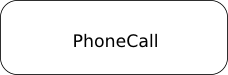
\includegraphics[scale=0.6,keepaspectratio=true]{./usability/federico1.png}
   \end{figure}
 \item Gerard Meszaros, in \textit{Pattern: Half Object + Protocol} suggested
that you should split that into half calls tied by a protocol.
   \begin{figure}[h!]
     \centering
     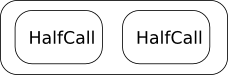
\includegraphics[scale=0.6,keepaspectratio=true]{./usability/federico2.png}
   \end{figure}
 We attain a local symmetry, we make a strong center, and get levels of scale.
 \item Now make a diagram of that:
   \begin{figure}[h!]
     \centering
     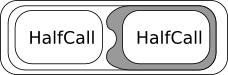
\includegraphics[scale=0.6,keepaspectratio=true]{./usability/federico3.png}
   \end{figure}
 You have local symmetry, levels of scale, boundaries, deep interlock and
ambiguity -- and this is where Meszaros left things.
 \item Richard Gabriel then suggests strengthening the centers that exist by
applying other structure-preserving transformations. What about the latent
center in the middle?
   \begin{figure}[h!]
     \centering
     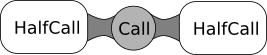
\includegraphics[scale=0.6,keepaspectratio=true]{./usability/federico4.png}
   \end{figure}
 You add an explicit boundary (Call) that ties the HalfCalls. This improves the
local symmetries, retains deep interlock and ambiguity, and it is composable.
 \item Yes, composable.
   \begin{figure}[h!]
     \centering
     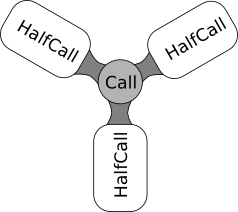
\includegraphics[scale=0.6,keepaspectratio=true]{./usability/federico5.png}
   \end{figure}
 Multi-way calls, conference calls, happen all out of applying
structure-preserving transformations.
\end{enumerate}
Probably every programmer keeps a mental picture of the program he is creating
or modifying. The hard part of modifying code that you did not write is forming
that mental picture in the first place. When you work to make the code present a
more beautiful picture, your code becomes better -- and Alexander gives us a good
way to do that.

\section*{The fundamental process}

Over a long argument, Alexander explains why following this process of applying
structure-preserving transformations is the \textbf{only} way to achieve a good,
functional design. This is not just for buildings, but for everything we
construct. It does not matter if you start with an existing program or building
or city, or whether you are starting from scratch. We mimic nature's own
evolutions and regenerative processes, but we do it faster.
\begin{enumerate}
 \item Start with what you have -- an empty lot, or an already-built building, or
a program that looks ugly and is hard to use.
 \item Identify the centers that exist in that space. Find the weakest center or
the least coherent.
 \item See how to apply one or more of the fifteen structure-preserving
transformations to strengthen that weak center. Does it need to be delimited?
Does it need to be blended with its surroundings? Does it need more detail? Does
it need to be de-cluttered?
 \item Find the new centers that are born when you apply the transformation to
the old center. Does the new combination make things stronger? Prettier? More
functional?
 \item Ensure that you did the simplest possible thing.
 \item Go back to the beginning for the next step.
\end{enumerate}
A super-simple summary would be: find the bad parts, make them better in the
simplest way possible, test the results, iterate.

Alexander is not keen on destroying things just to rebuild them in a different
way. You should  not demolish parts of a town to rebuild it; you should improve
it gradually. In software, it is well-known that you should not rewrite things
just because you do not understand them anymore. Tearing things down makes you
lose all the knowledge you had embodied in the thing you are destroying, even if
it looks ugly in its current state.

Similarly, Alexander is against making detailed, up-front designs. He gives a
good argument of why pre-made designs can not work well in the end: because you
can not predict absolutely everything that will come up during construction or
implementation; because you will miss details of the environment into which your
creation will live; because nature itself is not pre-ordained, and rather it
grows organically and mercilessly evolves things until they manage to survive by
themselves.

In this fashion, you do not design the whole user interface, or the whole
structure, for a big program in a single step. You go from big to small or small
to big (levels of scale); you test each part individually until it is good
(strong centers); you make sure the parts are not too disconnected from each
other (non-separateness). You move a few widgets where they are easier to reach,
or where they are closer to the data to which they refer. You remove some frames
and separators to reduce clutter. Above all, you continually evaluate what you
created against real users and real use cases, so that you empirically test
things against reality, not against castles in the sky.

\section*{A Name for the Quality}

Over the course of \textit{The Nature of Order}, Alexander manages to show that
environments or structures that are built according to that method all end up
having the Quality Without A Name. He calls this \textbf{living structure}. It
can be measured and compared. It no longer has no name; we can now speak of
environments with more or less living structure than others, or of programs with
more or less living structure than others -- and we strive to make and have more of
that property.

I just called this essay, ``Software that has the Quality Without A Name'' because
it sounds more mysterious that way.

I can not claim to know the perfect way of designing and writing software now,
but at least I have a good method grounded on what produces good things
elsewhere. It worked for my house, and so far I have seen it work very well for
my software. I hope it works well for you, too!


\section*{References}
\begin{itemize}
 \item Christopher Alexander, \textit{A Pattern Language}. Online version at
\url{http://bit.ly/8n6igg}
 \item Christopher Alexander, \textit{The Nature of Order}. Terrible web page at
\url{http://www.natureoforder.com}
 \item Photos and drawings of the fifteen properties of life -
\url{http://bit.ly/b82Dxu}
 \item Richard Gabriel, \textit{Patterns of Software}. A beautiful, wide-ranging
book on software development, Christopher Alexander's ideas, and the search for
good techniques for writing software. Online version at
\url{http://bit.ly/dqGUp4}
 \item Richard Gabriel, \textit{Christopher Alexander: the search for beauty}. A
very good presentation of Christopher Alexander's ideas and an exposition of
patterns in the software world.
\url{http://bit.ly/ztE6cp}
 \item Richard Gabriel, \textit{The Nature of Order: the post-patterns world}.
Another very good presentation, subsequent to the previous one, that explains
the Fifteen Properties of Life, the Fundamental Process, and how this relates to
software. \url{http://dreamsongs.com/Files/NatureOfOrder.pdf}
 \item Federico Mena Quintero, \textit{Software that has the Quality
   Without A Name}.  Presentation for the 2011 Desktop Summit in
   Berlin.  \url{http://bit.ly/oYgJUf}
\end{itemize}

\part{Artwork and Design}
\chapterwithauthor{Máirín Duffy Strode}{Don't Be Shy}

\authorbio{Máirín Duffy Strode has been using Free and Open Source software since she
was in high school, and has been a contributor for the past 8 years. She is involved
in both the Fedora and GNOME communities and has worked on interaction design,
branding, and/or iconography for a number of prominent FOSS applications such as
Spacewalk, Anaconda, virt-manager, SELinux and SSSD. She has also been involved
in outreach efforts teaching children design skills using FOSS tools such as
GIMP and Inkscape and is a fierce advocate for said tools. She is the team lead
of the Fedora Design Team and a senior interaction designer with Red Hat, Inc.}

\noindent{}I knew about and used Free and Open Source software for a long time before I
became a contributor. This was not for lack of trying -- there were a couple of
false starts, and I succumbed to them mostly out of being too shy and afraid to
push through them. From the aftermath of those false starts and also from
on-boarding other designers in FOSS projects, I have five tips to offer to you
as a designer trying to ramp up as a FOSS contributor:

\section*{1. Know that you are needed and wanted (badly!)}

My first false start happened when I was a first-year computer science student
at Rensselaer Polytechnic Institute. There was a particular project I used a lot
and I wanted to get involved with it. I did not know anyone in the project (or
anyone who was involved in free software) so I was trying to get involved pretty
cold. The project's website indicated that they wanted help and that they had an
IRC channel, so I lurked in there for a week or two. One day after a lull in
conversation, I spoke up: I said I was a computer science student interested in
usability and that I would love to get involved.

``Go away'' was the response. Furthermore, I was told that \emph{my} help was not
needed nor wanted. 

This set me back a few years in getting involved -- just a few harsh words on IRC
made me afraid to try again for almost 5 years.  I did not discover until much
later that the person who had essentially chased me out of that project's IRC
channel was on the fringes of the project and had a long history of such
behavior, and that I really had not done anything wrong. If I had only kept
trying and talked to other people, I may have been able to get started back
then.

If you would like to contribute to Free and Open Source software I guarantee you
there is a project out there that really needs your help, especially if you are
design-minded! Are you into web design? Iconography? Usability? Skinning? UI
mockups? I have spoken to many FOSS developers who are not only desperate for
this kind of help, but who would also deeply appreciate it and love you to
pieces for providing it.

If you encounter some initial resistance when first trying to get started with a
project, learn from my experience and do not give up right away. If that project
turns out to not be right for you, though, do not worry and move on. Chances are,
you are going to find a project you love that loves you back.

\section*{2. Help the project help you help them}

Many Free and Open Source Software projects today are dominated by programmers and
engineers and while some are lucky enough to have the involvement of a creative
person or two, for most projects a designer, artist, or other creative's
presence is an often-yearned-for-yet-never-realized dream. In other words, even
though they understand they need your skills, they may not know what kinds of
help they can ask you for, what information they need to give you to be
productive, or even the basics of how to work with you effectively. 

When I first started getting involved in various FOSS projects, I encountered
many developers who had never worked directly with a designer before. At first,
I felt pretty useless. I could not follow all of their conversation on IRC
because they involved technical details about backend pieces I was not familiar
with. When they bothered to pay attention to me, they asked questions like,
``What color should I put here?'' or ``What font should I use?'' What I really
wanted as an interaction designer was to be privy to decision-making about how
to approach the requirements for the project. If a user needed a particular
feature, I wanted to have a say in its design -- but I did not know when or where those decisions were happening and I felt shut out.

Design contains a pretty wide range of skills (illustration, typography,
interaction design, visual design, icon design, graphic design, wordsmithing,
etc.) and any given designer likely does not possess all of them. It is
understandable, then, that a developer might not be sure what to ask you for.
It is not that they are trying to shut you out -- they just do not know how you
need or want to be involved.

Help them help you. Make it clear to them the kind of work you would like to offer by providing samples of other work you have done. Let them know what you need so they can better understand how to help you engage in their project. For example -- when you first get involved in a particular initiative for the project, take the time to outline the design process for it, and post it on the main development list so other contributors can follow along. If you need input at particular points in the process, flag those points in your outline. If you are not sure how particular things happen -- such as the process for developing a new feature -- approach someone on the side and ask them to walk you through it. If someone asks you to do something beyond your technical ability -- working with version-control, for example -- and you are not comfortable with that, say so.

Communicating your process and needs will prevent the project from having to
make guesses and instead they will be able to make the best use of your talents.

\section*{3. Ask questions. Lots of questions. There are no stupid questions.}

We have noticed sometimes in Fedora that when new designers come on board, they
are afraid to ask technical questions for fear they will look stupid. 

The secret is, developers can be so specialized that there are a lot of
technical details outside of their immediate expertise that they do not
understand either -- this happens even within the same project. The difference is that they are not afraid to ask -- so you should not be, either! In my interaction design work, for example, I have had to approach multiple folks on the same project to understand how a particular workflow in the software happens, because it is passed off between a number of subsystems and not every person in the project understands how every subsystem works. 

If you are not sure what to work on, or you are not sure how to get started, or
you are not sure why that thing someone said in chat is so funny -- ask. It is a
lot more likely someone is going to tell you that they do not know either, than
they are going to think that you are stupid. In most cases, you will learn
something new that will help make you a better contributor.

It can be especially effective to seek out a mentor -- some projects even have
mentoring programs -- and ask them if they would not mind being your go-to person when you have questions. 

\section*{4. Share and share often. Even if it is not ready yet. Especially if it
is not ready yet.}

We have also noticed new designers in Fedora and other Free and Open Source projects
are a little shy when it comes to showing their work. I understand that you
do not want to ruin your reputation by putting something out there that is not
your best or even finished, but a big part of how Free and Open Source projects
work is sharing often and openly. 

The further along you have come on a piece before you have shared it, the harder
others will find it to provide you actionable feedback and to jump in and get
involved. It is also harder for others to collaborate on your piece themselves
and feel a sense of ownership for it, supporting and championing it through to
implementation. In some Free and Open Source projects, not being forthcoming with
your sketches, designs, and ideas is even seen as offensive! 

Post your ideas, mockups, or designs on the web rather than in email, so it is
easy for others in the project to refer to your asset via copying and pasting the
URL -- especially handy during discussions. The easier it is to find your design
assets, the more likely it is they will be used. 

Give this tip a try and keep an open mind. Share your work early and often, and
make your source files available. You might be pleasantly surprised by what
happens!

\section*{5. Be as visible as you can within the project community.}

One tool that -- completely unintentionally -- ended up helping me immensely in
getting started as a FOSS contributor was my blog. I started keeping a
blog, just for myself, as a sort of rough portfolio of the things I had been
working on. My blog is a huge asset for me, because:
\begin{itemize}
 \item As a historical record of project decisions, it is a convenient way to look up old design decisions -- figure out why we had decided to drop that screen again, or why a particular approach we had tried before did not work out, for example.
 \item As a communication device, it helps other contributors associated with your
project and even users become aware of what work is happening and aware of
upcoming changes in the project. Many times I have missed something essential in a design, and these folks have been very quick to post a comment letting me know!
 \item It helped me to build my reputation as a FOSS designer, which has helped me build others' trust in my design decisions as time has gone on. 
\end{itemize}

Do you blog? Find out which blog aggregations the members of the
project you are working on read, and put in requests to have your blog
added to them (there is usually a link to do so in the sidebar.) For example, the main blog aggregator you will want to join to become a part of the Fedora
community is called Planet Fedora\footnote{\url{http://planet.fedoraproject.org}}. Write a first blog
post once you have been added introducing yourself and letting folks know what you like -- all of the sort of information advised in tip \#1.

The project will surely have a mailing list or forum where discussion takes
place. Join it, and send an intro there too. When you create assets for the
project -- no matter how small, no matter how unfinished -- blog about them,
upload them to the project wiki, tweet/dent about them, and send links to
prominent community members on IRC to get their feedback.

Make your work visible, and folks will start to associate you with your work and
approach you with cool projects and other opportunities based solely on that.


This is everything I wish I had known when first trying to get involved in Free
and Open Source software as a designer. If there is any one thing you should
take away from this, it is that you should not be shy -- please speak up, please
let your needs be known, please let others know about your talents so they can
help you apply them to making Free Software rock.

\chapterwithauthor{Eugene Trounev}{Use of Color and Images in Design Practices}

\authorbio{An active member of Free Software and KDE for about 6 years, Eugene
Trounev started in KDEGames and followed through the entire KDE3-to-KDE4
transition. Nowadays he is mostly taking care of KDE's web presence and main
desktop appearance.}

\noindent{}Since the most ancient times people have used the power of images and color to
pass information, draw attention, and distract attention. The infamous
saying goes ``A picture is worth a thousand words'', and it could not be more to
the point. From the way we dress, to flashy neon light of downtown stores across
the globe -- every color, every shape and every curve has a purpose.

Knowing the purpose however is not that hard, since all of those variations of
hues and lines are put together to be read and felt by every one of us. It is
true therefore that a great design must come straight from the heart, as it is
supposed to speak to the heart in the first place. Nonetheless, just the heart
alone would not be able to make a great design, if some rules are not set and
followed at first.

\section*{Colors and textures}

There are many different ways to classify the colors into categories, but many of
them focus on physical or chemical properties of light or ink, and though they are
important in the end, those will not help you make an appealing design. The one way
that I found works best is to split colors into warm and cool. Simply speaking,
warm colors are those closer to the shade of red. They are: red, orange and
yellow. Cool colors, on the other end, are the ones running towards blue. They are: green,
blue and to a lesser extend violet. It is important to remember that cool is
also calm and breathy, while warm is impulsive and dangerous. So, depending on
what feelings you wish to awaken within your audience, you should use either
warmer or cooler colors. Draw attention with warm and inform with cool.
Overuse of either will result in either overheating -- creating negative feelings
in your viewer, or freezing-over -- causing indifference.

It is important to remember that black, white and grays are colors, too. These,
however, are neutral. They cause no feeling, but rather set an atmosphere. The
properties of these will be discussed later.

Every image is first and foremost a collection of colors, and as such will abide
by the rules of color management. Determining the dominant color of your image is
the key to success. Try to see the big picture, and do not concentrate on
details. A good way to do this is by setting an image against some dark
background, then taking a few steps back and observing it from a distance. Which
color do you see the most of?

Not all images have a dominant color, however. Sometimes you may come across
color bloat, where no matter how hard you look you can not determine which hue
dominates. Try to avoid such pictures, as they will inevitably confuse your
viewer. When confronted with imagery like that, people tend to look away quickly
and it will not give a good impression, no matter what it speaks of.

Beside color, pictures also have a texture, as ultimately they are nothing but a
collection of textured colors. Detecting the dominant texture of an image is not as
straight forward as its color, as textures are seldom obvious, especially in
photographs. There are however a few pointers to help you. Human nature causes
us to be drawn to curved, so called ``natural'' shapes, while angular,
sharp-looking shapes are considered less attractive. That is why an image of a
curved, green leaf would appeal to more people then that of a metal spike.

To summarize: the key to a successful, appealing design is a good, well
balanced combination between color and texture in the images used.

\section*{Texts and spaces}

An equally important aspect of any good design is the use of text and
spaces around it. And just like it is with the image textures and color, you
should always remember that people like to breathe. This means that there should be
sufficient space in and around the text to make it easier to spot, read and
understand.

Consider an example of two pages -- one coming from a romantic novel, while the
other is taken straight from a legal document. You would most likely prefer the
romantic novel over a legal document any day, but do you know why? The answer is
simply because you like to breathe. A page from any romantic novel is likely to
contain three important elements: a) conversations; b) paragraphs; c) extra wide
margins, while most legal documents normally contain neither. All of the
aforementioned elements make the page feel alive and dynamic, while the absence
of those make it look like a solid wall of text. Human eyes, being more
accustomed to a certain degree of variety of sights, feel more at ease when
presented with spacious, fluid layouts.

This does not however imply that every text must have all those three elements in
order to seem more attractive. Far from it. Any text can be made easy and
enjoyable by injecting enough air into the flow.

Air, or space, can come through a variety of ways, such as: letter, line and
paragraph spacing; content, section, and page margins; and finally letter size. Try
to keep at least one character-tall space between your paragraphs and lines, and
two character-tall space between sections in your text. Allow generous spacing
around the text on a page by setting your margins wide enough. Try to never go
below 10-points font size for your paragraph text, while keeping headings large
enough to stand out.

\section*{Attraction and information}

Just like animals, human beings are often attracted by bright splotches of color
and unusual texture, and the more captivating the sight is, the more oblivious
people become towards other potential points of interest. This simple rule of
attraction has been used since the most ancient times by females and males
alike to drive the attention of others away from certain things they did not want
to be noticed. The best example of such a trickery is the work of a street
magician, who often distracts viewers’ attention by use of smoke, flames or
flashy attire.

It is important to remember here that words are visual too, as they produce
specific associations and visions. The very same trick that can be done with
smoke and fires can also be achieved through creative use of wording. By far the
best example of a trickery done with words is our every day price tags. Ever
wondered why retailers love those .99s and .95s so much? That is because \$9.95, or
even \$9.99 looks more attractive than \$10.00, even though in reality they
have the same impact on your wallet. Trow an ``old'' \$10.00 price tag noticeably
crossed through with a thick red line into the mix and you got yourself a great
customer magnet.

\section*{Conclusion}

Great, attractive design is achieved by following these simple rules: a) choose
your imagery wisely; b) make good use of colors and textures to create an
atmosphere; c) give your viewer some room to breathe; d) draw the attention
away from the parts that matter the least, and towards those that matter the
most.

This short essay is not meant to cover the whole wide spectrum of various design
styles, techniques and rules, but rather to give you -- the reader -- a starting
point you could carry on building upon.

\part{Community Management}
\chapterwithauthor{Robert Kaye}{How Not to Start a Community}

\authorbio{Robert Kaye combines his love for music and open source into the open
music encyclopedia MusicBrainz. Robert founded and leads the California-based
non-profit MetaBrainz Foundation in a long term effort to improve the digital
music experience. Beyond hacking on MusicBrainz, Robert seeks out interesting
festivals like Burning Man and interesting side projects like hacking on
drink-mixing robots. Topped with a colorful hair style at all times, you will
never have a hard time picking him out of a crowd.}

\noindent{}In 1998, I was working at Xing Technology in San Luis Obispo, working hard on
our new AudioCatalyst project. It was one of the first integrated MP3 ripping
programs that made use of the CDDB database. CDDB was the CD database that
allows any player to look up the title and tracklisting for any CD. If the CD
was not listed, you could enter the data so that the next person could make use
of the data. I loved this online collaborative project and typed in several
hundred CDs over the course of a few years.

One day we were notified that CDDB had been purchased by Escient, a company that
would later become GraceNote. The CDDB database was taken private so that people
could no longer download the complete database! And on top of that Escient did
not compensate any of the contributors for their efforts; they were ripping off
the general public with this move. I was quite angry with this move and still am
to this day.

A few months later we were notified by Escient that we would be required to play
the Escient jingle and display the Escient logo when making a CD lookup in our
products. That was it! Now I was livid! Later that week at a party with friends
I was complaining about what was happening and how unhappy I was. My friend
Kevin Murphy said to me: ``Why don’t you start your own open source project to
compete with these bastards?''

A few weeks later I stopped working for Xing and had a couple of weeks of spare
time before I would start at EMusic. I decided to teach myself Perl and web
programming and set out to create the CD Index, a non-compatible, non-infringing
project to compete with CDDB. I hacked on the project during the break, but then
promptly forgot it once I became a member of the FreeAmp project at EMusic.

Then in March of 1999 Slashdot asked what the open replacement for CDDB was
going to be. I spent the rest of that day and most of the night finishing the CD
Index and deploying it. I submitted a Slashdot story about my
project\footnote{\url{
http://slashdot.org/story/99/03/09/0923213/OpenSource-Alternative-to-CDDB}} and
it promptly posted. As expected, thousands of geeks showed up within minutes and
my server tipped over and died.

The masses of people who arrived immediately started shouting for things to
happen. There was not even a mailing list or a bug tracker yet; they insisted on
having one right now. Because I was new to open source, I did not really know
what all was needed to launch an open source project, so I just did as people
asked. The shouting got louder and more people insisted that I shut the service
down because it was not perfect. Even amidst the mess, we received over 3000 CD
submissions during the first 24 hours.

Once things calmed down, there were still plenty of people shouting. Greg Stein
proclaimed that he would write a better version immediately. Mike Oliphant,
author of Grip, said he was going to work on a new version as well. Alan Cox
came and loudly proclaimed that SQL databases would never scale and that I
should use DNS to create a better CD lookup service. Wait, what?
I was very unhappy with the community that grew out of the Slashdot posting. I
did not want a place were people could treat each other without respect and
people who felt entitled could shout louder until they got what they wanted. I
quickly lost interest in the project and the CD Index faltered. The other
projects that people promised they would start (not counting FreeDB) never
materialized.

Then when the dot com bust started, I needed to think about what I would do
next. It was clear that my job at EMusic was not safe; still I was driving a
Honda S2000 roadster, my dot com trophy car. With car payments double my rent, I
had to decide: Work on my own stuff and sell my dream car, or move to the Bay
Area and work on someone else’s dream, if I could even find a job there.

I decided that a comprehensive music encyclopedia that was user-generated would
be the most interesting thing to work on. I sold the S2000 and hunkered down to
start working on a new generation of the CD Index. At yet another party, the
name MusicBrainz came to me and I registered the domain in the middle of the
party. The next day, motivated by the project’s new name, I started hacking in
earnest and in the Fall of 2000 I launched musicbrainz.org.

Launched is not the right term here -- I set up the site quietly and then
wondered how I could avoid another Slashdot-based community of loud screaming
kids. I never imported data from the CD Index, nor did I mention MusicBrainz on
the CD Index mailing lists. I simply walked away from the CD Index; I wanted
nothing more to do with it. In the end I decided to add one simple button to the
FreeAmp web page that mentioned MusicBrainz.

And a very strange thing happened: people came and checked out the project. It
was very few people at first, but when a person mentioned something to me, I
would start a conversation and gather as much feedback as I could. I would
improve the software based on feedback. I also set a tone of respect on the
mailing lists, and every time someone was disrespectful, I would step in and
speak up. My efforts directed the focus of the project towards improving the
project. I did this for over 3 years before it became clear that this approach
was working. The database was growing steadily and the data quality went from
abhorrent to good over a number of years. Volunteers come and go, but I am the
constant for the project, always setting the tone and direction for the project.
Today we have a 501(c)3 non-profit with 3.25 employees in 4 countries, Google,
the BBC and Amazon as our customers and we are in the black. I doubt that could
have happened with the CD Index community.

I wish I would have known that communities need to grow over time and be
nurtured with a lot of care.

\chapterwithauthor{Jono Bacon}{Hindsight is Almost 20/20}

\authorbio{Jono Bacon is a community manager, engineering manager, consultant and author.
Currently he works as the Ubuntu Community Manager at Canonical, leading a team
to grow, inspire and enthuse the global Ubuntu community. He is the author of
Art of Community, founder of the Community Leadership Summit and co-founder of
the popular podcast LugRadio.}

\noindent{}I first learned of Linux and Open Source back in 1998. While the technology was
gnarly and the effort required to get a smooth running system was significant,
the concept of this global collaborative community transfixed me. Back then I
had no knowledge, limited technical skills, and zits.

As an angsty teenager complete with long hair and Iron Maiden t-shirt, my path
was really already mapped out for me in the most traditional sense; I would go
to school, then college, then university, and then a job.

Fourteen years later, the path I actually took was by no means traditional, and
that intrinsic fascination with community has taken me around the world and
thrown me into some engrossing challenges. It is interesting to sit back and
reflect on this period of time. Well, it might be interesting for me\dots\ you
might want to skip to the next chapter\dots 
\newline
\dots
\newline
Still with me? OK, let’s roll.

\section*{Science vs. Art}

I have always believed that community management is less of a science and more
of an art. I define science as exploring methods of reproducing phenomena
through clearly understood and definitive steps. In the science world if you
know the theory and recipe for an outcome, you can often reproduce that outcome
like anyone else.

Art is different. There is no recipe for producing an incredible song, for
creating an amazing painting, or sculpting a beautiful statue. Similarly, there
is not really any reproducible set of steps for creating a thriving community.
Sure, there are tricks and techniques for achieving components of success, but
the same happens for other art-forms; we can all learn the notes and chords on a
guitar, it does not mean you are going to write the next Bohemian Rhapsody. The
formula that generates Bohemian Rhapsody is one part learned skill and one part
magic.

Now, I am not suggesting that community management is this frustratingly hip and
introverted artform that only the blessed few with such talents can achieve.
What I am instead lamenting is that there is no playbook for how to create a
wonderful and inspiring community; it is still one part learned skill and one
part magic, but the magic part is not divinely anointed to you by the gods, but
instead obtained by trying new things, being receptive to feedback, and getting
a feel for what works and what does not.

Rather frustratingly, this means that there is no single recipe to follow for
the magic, but there is still an opportunity to share the learned skills, as I
have sought to do with The Art of
Community\footnote{\url{http://artofcommunityonline.org}} and the annual
Community Leadership
Summit\footnote{\url{http://communityleadershipsummit.com}}.

Before I get started reflecting, and for those of you who have not bored
yourself into oblivion by following my career, I will summarize the communities
I have worked with so we can define the context. In a nutshell, I started out in
my hairier days by producing one of the UK’s first Linux community websites
called Linux UK and got involved in the Linux User Group (LUG) community. I went
on to create my own LUG in Wolverhampton in the UK and founded the Infopoint
project to encourage LUGs to advocate Linux at computer fairs across the UK. I
then went on to contribute to the KDE community, founded the KDE::Enterprise
site, got the KDE Usability Study going, and contributed to a few little apps
here and there. I then founded the PHP West Midlands user group and started also
getting interested in GNOME. I wrote a few apps (GNOME iRiver, XAMPP Control
Panel, Lernid, Acire) and also co-designed and wrote some code for a new
simplified audio app called Jokosher. Around this time I co-founded the LugRadio
podcast which would run for four years with over two million downloads and
spawning five live events in the UK and USA. At this time I also started work as
an Open Source consultant at the government-funded OpenAdvantage where I really
got a chance to cut my teeth in community and working with organizations across
the West Midlands to help them to move to Open Source. After a few years at
OpenAdvantage I moved on to join Canonical as the Ubuntu community manager and
developed a team of four and together we are involved in a wide variety of
projects in Ubuntu and Canonical.
\newline
Still with me?
\newline
Wow, you are persistent. Or bored. Probably bored. There will be an exam at the
end; that’ll teach you\dots

\section*{Reflecting}

So this brings me to the focus of this piece -- the curious question of if I knew what I did today, what would I tell myself? Over the course of my career so far I believe that everything I have learned can be boiled into two broad buckets:
\begin{itemize}
 \item Practical -- the tips and tricks of the trade; e.g. approaches to
communication mediums, using technology in different ways, event planning
techniques, project management approaches etc.
 \item Personal -- core life lessons and learnings that affect the approach you
take to your world.
\end{itemize}
I am not going to talk much about the practical -- you should read my
book for more on that topic (the book also covers a lot of the personal too).
Today I am instead going to focus on the personal life lessons. Approaches and
practices will always change, but the life lessons do not so much change but
grow and evolve as we get wiser.

\section*{The Importance Of Belief}

Communities are fundamentally networks of people driven by belief. Every
community has an ethos and a focus. This could be something as grandiose as
documenting all human knowledge or changing the world with Free Software, or it
could be as humble as providing a local group for people to get together to talk
about their favorite books. Whether life changing or just a bit of fun, each
community has a belief system; the humble book club still sees tremendous value
in providing a fun, safe and free environment to share reading preferences and
recommendations. It might not change the world, but it is still a good thing and
something people can get behind.

The underlying often unwritten rule of community is that every contribution from
a community member must benefit the wider community. This is why it is fun to
write a patch that fixes a Free Software bug, contribute documentation, run a
free event or otherwise, but it is rare that anyone is willing to contribute as
a volunteer if their contribution only benefits a single person or company.

Of course, I am sure all of you cynical bastards are now going to try and find
an exception, but remember that this decision is typically deeply personal --
the community member decides how comfortable they are that their contribution
will benefit everyone. As an example, some would argue that any contribution to
Mono would only benefit Microsoft and the ubiquity of their .NET framework, but
hundreds of contributors participate in Mono because they do not see it this way
-- they see their contributions as a valuable and fun way of making it easy to
empower Free Software developers to write Free Software more easily.

If I was talking to the Jono of 1998 I would really emphasize the importance of
this belief. I had a hunch about it back then, but I have since seen countless
examples of belief truly inspiring people to participate. I have often talked
about the story of the kid from Africa who emailed me to tell me how he would
walk three hours to and from his nearest Internet cafe to contribute to Ubuntu.
He did this because he believed in our mission to bring Free Software to the
masses. The same can be said for the tremendous growth in Wikipedia, the
incredible coming together of the GNOME community around GNOME 3, the success of
OpenStreetMap and many other examples.

Belief though is not a PR stunt. It has to be real. While each of us has
different belief systems, some map their belief systems to software, some to
education, some to knowledge, some to transparency or whatever else, you can not
concoct a belief system unless it serves a valid goal that a group are likely to
care about. Sure, it can be obscure, but it has to be real. With the success of
Open Source, we have seen some examples of some companies trying to use similar
language and approaches around belief, but applying it to self-serving needs. I
could invent a belief of ``let’s all work together to help Jono get rich'' and
concoct some nonsense of the benefits of this belief (e.g. if I am rich I can
focus on other work that would benefit other communities, my future kids would
get a wonderful education and upbringing and this will benefit the world), but
it would be rubbish.

As such, belief is a strong driver for collaboration and contribution, but it
must be met with respect and balance. While it can be a trigger for incredible
change, it can also be hugely destructive (e.g. some television preachers who
use religion as a means for you to give them money, or fake psychics who use
cold reading to latch onto your belief to desperately try and re-connect with a
lost loved one).

\section*{Your Role}

Community managers play an interesting role these days. In the past I have
talked about there being two types of community managers; those who go out and
give presentations and wave their hands around talking about a product or
service, and those who work with a community of volunteers to help them to have
a fun, productive and enjoyable collaborative experience. I am more interested
in the latter -- I feel that is what a real community manager does. The former
is a fine and respectable position to have, but it is more in the area of
advocacy and public relations, and requires a different set of skills. I have a
few tips here I think are interesting enough to share.

The first and probably most important lesson is having a willingness to accept
that you can and will be wrong sometimes. In my career so far I have got some
things right and some things wrong. While I believe I am generally on the right
path and most of my work is successful, there have been a few turkeys here and
there. These screw-ups, mishaps and mis-steps have never been out of
maliciousness or carelessness, they have instead typically been from me
overshooting the target of what I was trying to do.

This seems like a pretty obvious point, but it gets less obvious when you have a
fairly public role. By and large, community managers are often seen as
representatives of a given community. As an example, I know that I am personally
seen as one of the public faces of Ubuntu, and with that responsibility comes
the public pressure of how people perceive you.

For some community leaders, having the spotlight shone on them causes a
defensive mechanism to kick in; they cringe at the idea of making mistakes in
public, as if the chattering masses expect a perfect record. This is risky, and
what has been seen in the past is that we get public leaders who essentially
never accept that they have made a mistake due to this fear of public ridicule.
This is not only a fallacy (we all make mistakes), but it also does not set a
good example to the community of a leader who is honest and transparent in both
the things they do well and the things they do less well. It is important to
remember that we often gain respect in people because of their acceptance of
mistakes -- it shows a well-rounded and honest individual.

I remember when I first became a manager at Canonical and at the time Colin
Watson and Scott James Remnant, two original gangstas from the very beginning of
Canonical and Ubuntu, were also managers on the Ubuntu Engineering Team. We
would have our weekly calls with our manager, Matt Zimmerman, and on these calls
I would hear Colin and Scott openly accepting that they were not good at this,
or had made a mistake with that; they were stunningly humble and accepting of
their strengths and weaknesses. As a rookie manager I was a little more
tight-lipped, but it taught me that this kind of openness and honesty is not
only good as a manager but as a community leader and since then I feel no qualms
in publicly admitting to mistakes or apologizing if I screw up.

\section*{Listening}

In a similar way, while openness to mistakes is important, another lesson is the
importance of being a good listener and learning from our peers. In many cases
our communities look to community managers and leaders as people who should
always be providing guidance, direction and active navigation of the project and
its goals. This is definitely a responsibility, but in addition to the voicing
of this leadership, it is also important to be a passive listener, providing
guidance where appropriate and learning new lessons and insight.

Our community members are not just cold, hard, machines who perform work; they
are living, breathing, human beings with thoughts, opinions, feelings and ideas.
I have seen many examples, and I have accidentally done this before myself,
where someone is so used to providing guidance and direction that they sometimes
forget to just sit down and listen and learn from someone else’s experience.
Every industry is filled with thought leaders and scholars ... famous people
who are known for their wisdom, but in my experience some of the most
revolutionary life lessons that I have learned have come entirely from
non-famous, day-to-day, meat-and-potatoes community members. Being a great
listener is not just important to help us learn and be better at what we do, but
it is critical in gaining respect and having a great relationship with your
community.

\section*{On vs. Off Time}

While on the subject of how we engage with our community, I have another
take-away that I only truly processed in my own mind fairly recently. Like many
people, I have a number of different interests that fill my days. Outside of
being married and trying to be the best husband I can be, and my day job as the
Ubuntu Community Manager, I also have projects such as Severed Fifth, the
Community Leadership Summit, and some other things. As you would naturally
expect, my days are committed to my day job -- I do not spend time at work
working on these other projects. As such, as you would naturally expect, when my
work day ends I start working on these other projects. The lesson here is that
it is not always clear to your community where the lines are drawn.

Over the years I have developed a series of online facilities that I use for my
work and viewpoints. My Twitter, identi.ca, Facebook pages, my blog, and some
other resources are where I talk about what I do. The challenge is that if you
take into account these public resources, my public representation of the Ubuntu
project, and the wealth of timezones across the world, it does not take an
Einstein to confuse whether I am writing about something as a Jono thing or a
Canonical thing.

This has caused some confusion. As an example, despite my repeated
clarifications, OpenRespect is not and never has been a Canonical initiative. Of
course, some idiots choose to ignore my clarification of this, but I can see how
the confusion could arrive nonetheless. The same thing has happened for other
projects such as Severed Fifth, The Art of Community and the Community
Leadership Summit, of which none are, or ever have been, part of my work at
Canonical.

The reason why I consider this a lesson is that I have seen, and at one point
shared, the view that ``of course it is a spare time thing, I posted that at 8pm
at night'' and shrug of concerns of the lines blurring. When you have a job that
puts you in a reasonably public position, you can not have the luxury of just
assuming that; you have to instead assume that people are likely to blur the
lines and you have to work harder to clarify them.

\section*{Don’t Travel Too Much}

On the topic of working for a company that employs you to be a community leader,
you should always be aware of the risks as well as the benefits of travel. This
is something I learned fairly early on in my career at Canonical. I would see
the same faces over and over again at conferences, and it was clear that these
folks had clearly communicated the benefits of travel to their employer, as I
had done, but I also came to learn the risks.

I would travel and it would not only be tiring work and emotionally exhausting,
but I would also be away from my email more, on IRC less, unable to attend many
meetings, and have less time to work on my work commitments. As such, my role
would largely become that of getting out and visiting events, and while fun,
this did not serve my community as well as it should have done. As such, I
fairly dramatically cut my travel -- in fact, I went to the Linux Collab Summit
a few days ago, and outside of Ubuntu events that I needed to attend, I had not
made it to conference for nearly a year. Now I feel the pendulum has swung a
little too far in the other direction, so it is all about balance, but I also
feel I serve my community better when I am able to take the time to be at the
office and be online and accessible.

\section*{Planning}

For some folks, the role of a community leader or community manager is one that
is less about pre-disposed structure and instead more interrupt-driven. When I
started out, I used to think this too. While there is absolutely no doubt that
you do indeed need to be interrupt-driven and able to respond to things that are
going on, it is also essential to sufficiently plan your work for a given period
of time.

This planning should be done out in the open where possible and serves a few
functions:
\begin{itemize}
 \item Shares plans -- it helps the community to understand what you are working
on and often opens up the doors for the community to help you.
 \item Offers assurances -- it demonstrates that a community leader is doing something.
Your community can see your active work happening. This is particularly
important, as much of the work of a community leader often happens out of the
view of the wider community (e.g. having a one-on-one conversation with a
community member), and this lack of visibility can sometimes generate concerns
that little is happening in key areas, when instead a lot is going on behind the
scenes.
 \item Communicates progress up and down the ladder -- this is relevant if you
are working for a company. Having some solid planning processes in place
demonstrates your active work to your management, and it also re-assures your
team that they will always know what to work on and create great value for the
community.
\end{itemize}
Over the years I have put more and more importance in planning, while still
retaining enough time and flexibility to be interrupt-driven. When I started as
the Ubuntu Community Manager my planning was fairly personal and ad-hoc -- I
took the pulse of the community, and I applied my time and resources to tend to
those areas as I saw fit.

Today I break goals into a set of projects that each span an Ubuntu cycle,
gather input from stakeholders, put together a roadmap, track work in
blueprints, and assess progress using a variety of tools and processes such as
my burndown chart, regular meetings, and more. While the current approach
requires more planning, it helps significantly with the benefits covered in the
above bullet points.

\section*{Perception and Conflict}

One thing I often hear about in the world of community management and leadership
is the view that perception is everything. Typically when I hear this it is in
response to someone getting the wrong end of the stick about something, often in
a conflict period.

Of course, perception does indeed play an important part in our lives, but what
can fuel incorrect or misaligned perceptions is lack of information,
mis-information, and in some cases, heated tensions and tempers. This can be
some of the most complex work for a community leader, and I have come away with
a few lessons learned in this area too.

Communities are groups of people, and in every group there are often common
roles that people fill. There is usually someone who is seen as a rockstar and
hero, someone who is sympathetic to concerns and worries and a shoulder to cry
on, someone who is overtly outspoken, and often someone who is ... well ...
deliberately difficult. Heroes, sympathetic ears and outspoken folks are not
particularly challenging, but deliberately difficult people can be complex; if
someone is being overtly difficult to deal with, it can cause tensions to form
with other members and bring conflict to an otherwise happy community. We need
to nip those issues in the bud early.

Part of the challenge here is that people are people, groups are groups, and it
is not uncommon for a single person or a few people to become known and
complained about behind closed doors as difficult to work with. In addition to
this, most people do not want to get involved in any conflict, and as such the
person being complained about can sometimes never actually know that people see
them this way, as no-one wants to confront them about it. This results in one of
the most dangerous situations for a community members -- a reputation is spread,
without the knowledge of the person who it applies to, and because they never
know, they never have an opportunity to fix it. That is a pretty sucky position
to be in.

A common response to this conclusion is the view that ``they are so difficult to
deal with that trying to reason with them will fall on deaf ears anyway''. While
this certainly does happen from time to time, do not be so quick to assume this
will be the outcome; there have been a few times when I have had the
uncomfortable experience of feeling I need to share with someone the reputation
that they have developed, and in virtually all cases it has been a real surprise
to them, and they have almost all modified their behavior based on the feedback.

On a related note, while often not a common part of the daily routine of a
community leader, conflict will often raise its head here and there. I just
wanted to share two brief elements about conflict.

The first is understanding how conflict forms. To introduce this, let me tell
you a little story. Last week a friend of mine flew out to the Bay Area for a
conference. He arrived in the evening, so I picked him up from the airport and
we went to the pub to catch up. While there he started telling me how
disappointed he was with Obama and his administration. He cited examples of
health care reform, Wall Street reform, digital rights and more. His agitation
was not with the policies themselves, but with Obama not doing enough. My
perspective was a little different.

I am not a democrat or a republican; I make my decisions on each issue, and I do
not align myself with either party. Where I differ to my friend though is that I
am a little more sympathetic to Obama and his daily work. This is because I
believe that he, and anyone else in a public position, whether as
internationally recognized as the president, or as obscure and specific as a
community manager, realizes that the story read and understood by the public is
often only a fragment of the full story. There have been cases in the past where
something controversial has kicked off in the communities that I have been a
part of, and many of the commentators and onlookers have clearly not had a full
knowledge of the facts either because they have not picked up on the nuances and
details of the topic or some parts of the story have not been shared.

Now, I know what some of you are going to say -- some parts not shared?! Surely
we should be transparent? Of course we should, and we should always strive to be
open and honest, but there are some cases when it would be inappropriate to
share some parts of the story. This could be because of private conversations
with people who do not want their comments shared, and also just being classy in
your work and not throwing dirt around. As an example, I have always had a very
strong policy of not throwing cheap shots at competitors, no matter what
happens. In the past there has been some questionable behavior from some
competitors behind the scenes, but I am not going to go out and throw dirt
around as it would not serve a particularly useful purpose, but with that I have
to accept that some community critique will only have part of the picture and
not be aware of some of the behind the scenes shenanigans.

Finally, on the topic of conflict, I believe a real life lesson I have learned
has been the approach in which critique and successful outcomes should be
approached. Although blogging has had a hugely positive impact on how people can
articulate and share opinions and perspectives, there has been a dark side.
Blogging has also become a medium in which much overzealous opinion can
sometimes be expressed a little too quickly. Unfortunately, I have a rather
embarrassing example of someone who fell into this trap: yours truly.

First, a bit of background. There used to be a company called Lindows that made
a version of Linux that shared many visual and operational similarities to
Windows. Microsoft frowned at the name ``Lindows'', and a fight started to
change the name. Lindows initially resisted, but after mounting pressure,
changed their name to Linspire.

Now to the issue. Let me take the liberty to explain in the words of the article
itself:
\begin{quote}
 Recently a chap named Andrew Betts decided to take the non-free elements out of
Linspire and release the free parts as another Linspire-derived distribution
called Freespire. This act of re-releasing distributions or code is certainly
nothing new and is fully within the ethos of open source. In fact, many of the
distributions we use today were derived from existing tools.

Unfortunately, Linspire saw this as a problem and asked for the Freespire name
to be changed. Reading through the notice of the change, the language and flow
of the words screams marketing to me. I am certainly not insinuating that Betts
has been forced into writing the page, or that the Linspire marketing drones
have written it and appended his name, but it certainly doesn’t sound quite
right to me. I would have expected something along the lines of ``Freespire has
been changed to Squiggle to avoid confusion with the Linspire product'', but
this is not the case. Instead we are treated to choice marketing cuts such as
``To help alleviate any confusion, I contacted Linspire and they made an
extremely generous offer to us all''. Wow. What is this
one-chance-in-a-lifetime-not-sold-in-stores offer? Luckily, he continues, ``they
want everyone who has been following my project to experience ‘the real’
Linspire, FOR FREE!!!''. Now, pray tell, how do we get this ‘real‘ version of
the software ``FOR FREE!!!''?

``For a limited time, they are making available a coupon code called ‘FREESPIRE’
that will give you a free digital copy of Linspire! Please visit
\url{http://linspire.com/freespire} for details''. Oh \dots\ thanks.
\end{quote}

I gave Linspire a pretty full-throated kick in the wedding vegetables in my blog
entry. I told the story, objected to what I considered hypocrisy given their own
battle with similar-sounding trademarks, and vented. I wish Guitar Hero had
existed back then: it would have been a better use of my time.

I was wrong. My article was never going to achieve anything. Shortly after the
article was published, then-CEO Kevin Carmony emailed me. He was not a happy
bunny. His objection, and it was valid, was that I flew off the handle without
checking in with him first. My blog entry was my first reaction. The reality of
the story was far less dramatic, and Linspire were not the ogres that I painted
them to be. I apologized to Kevin and felt like an idiot.

Many conflict scenarios are resolved in private discussions where people can be
open and focus on solutions without the noise. Over the years I have seen many
examples of a furious public blogging war going on while behind the scenes there
is a calm exchange of opinions and the focus on solutions.

\section*{Wrapping Up}

When I started writing this it was much shorter, but I just kept adding one more
thing, and then one more thing and so on. It is already long enough that I can
probably count the number of people reading this bit on one hand, so I am going
to hang it up here. I could go on forever with little tidbits and experiences
that I have been fortunate enough to be involved in and expand my horizons, but
then I would end up writing The Art of Community II: This Time It's Personal.

Life is a constant on-going experience, and I hope your investment in reading
this has added to it a little.

\chapterwithauthor{Alexandra Leisse}{Things I'm Happy I Didn't Know}

\authorbio{Alexandra Leisse left one stage to enter another and turn her other passion --
software and the web -- into a profession. After a transition period of 12
months of freelancing both in software and opera -- and sinking countless hours
into KDE activities, she joined Nokia, Qt Development Frameworks as Web
Community Manager.
\newline
She is the woman behind the Qt Developer Network and Qt’s community activities
on the web. Despite holding a degree in opera performance, she mostly refuses to
sing in public.}

\section*{Introduction}

When Lydia asked me to join her book project under the working title of ``things
I wish I had known'', my mind went blank. Things I wish I had known but didn't?
Nothing came to mind.

I am not saying that I didn't need to learn anything, on the contrary. I had to
learn a lot and I made countless mistakes. But situations or mistakes I would
have preferred to avoid? I can't think of any.

All of us have the annoying tendency to look at the things that we could do
better, the things we do not know, and perceive them as weaknesses. But what
about weaknesses that are our strengths?

Here is my personal story about ignorance, naivety and false perception, and
about how happy I am I had no clue.

\section*{Names}

I had no idea who this guy was I met during the first day of my job. He entered
the room, introduced himself, and started asking tough questions that gave me
the impression that all I thought I would be doing was nonsense. He was
apparently well informed about my doings in KDE and the people I used to deal
with. Still we seemed to have different standpoints. At some point I grew tired
of his provocations and lost patience. I told him that things are not always as
easy with people as engineers wish they were.

It was only after he had left after about an hour of discussing that I googled
his name: Matthias Ettrich. What I read explained a lot about why he asked the
questions he did. If I had known before that he is one of the founders of the
KDE project I would have likely argued in a very different way -- if at all.

I had to look up quite some names during the last years, and I was happy every
single time that I did it \textit{after} the first contact.

This is probably my most important point. When I met all these FOSS people for
the first time I had almost never heard their names before. I did not know about
their history, their merits, nor their failures. I approached everyone in the
same way: on eye-level. 

By being ignorant (or naive, as some have called it), I did not feel inferior to
the people I met when I started my journey into FOSS land. I knew I had a lot to
learn but I never had the impression I had a lower position than others as a
person.

\section*{``High-Profile-Project''}

I had not religiously followed dot.kde.org nor PlanetKDE, let alone all those
countless other FOSS related publications before I started lurking on KDE
mailing-lists. I perceived those channels first and foremost as means of
communication to a very select audience, mainly users of and contributors to the
project itself. 

For quite some time, it did not even cross my mind that the articles I published
on The Dot might be picked up by journalists. I put an effort into writing them
because I wanted to do a good job rather than because I was afraid of making a
fool out of myself in the world's face. The press list was maintained by other
people and what I wrote did not appear that important to me either. I wanted to
reach certain people, and the official channels and my own blog seemed like the
most efficient way of doing it.

Being quoted on ReadWriteWeb after announcing on my blog that I would start a
new job almost came as a shock to me. It is not that I did not know that people
read what I write -- I certainly hope they do! -- I simply did not expect it to
be that much of a topic. It wasn't even summer break.

Good thing nobody told me; I would not have been able to publish a single line.

\section*{The Outsider}

Some time ago when I attended my first conference I did so with the firm belief
that I was different from the other attendees. I saw myself as an outsider
because I did not have much in common with anybody else apart from a fuzzy
interest in technology: I had been freelancing for some years already after
graduating from university, I had no relevant education in the field, and I was
mother of a 10 year-old child. On paper at least, it could not get much
different from the usual suspects one meets inside FOSS projects.

In 2008 I attended a KOffice sprint as part of the KDE marketing and promotion
team to prepare the 2.0 release. The initial idea was to sketch out a series of
promotional activities supporting the release to grow both developer and user
base, for which there were three of us running a parallel track to the developer
discussion.

We tried to understand how we could position KOffice and adapt communication to
the intended audience. Pretty soon in the process, we discovered that we had to
take a step back: at that point, the immaturity of the suite made it impossible
to position it as an option for unsuspecting users. We had to stick with
developers and early adopters. It was a tough sell to some of the developers but
as outsiders we had the chance to look at the software without thinking of all
the blood, sweat and tears that went into the code.

For a lot of projects, no matter of which kind they are, the core contributors
have a hard time taking an objective look at the state of affairs. We tend to
not see the great accomplishments while we are so focused on the issues in
detail, or the other way around. Sometimes we miss a good opportunity because we
\textit{think} it has nothing to do with what we are doing -- or that no-one
would want this in the first place.

In all these cases, people outside the project have the potential to inject some
different viewpoints into the discussion, particularly when it comes to
prioritization. It is even more helpful if they are not developers themselves:
they will ask different questions, will not feel pressured into knowing and
understanding all technical details, and they can help decisions and
communication on a higher level.

\section*{Conclusion}

Ignorance is bliss. It is not only true for the individuals who benefits from
the fearlessness that results from a lack of knowledge but also for the projects
these individuals join. They bring different views and experiences.

And now, go and find yourself a project that interests you, regardless of what
you think you know.


\part{Packaging}
\chapterwithauthor{Jonathan Riddell}{From Beginner to Professional}

\authorbio{Jonathan Riddell is a KDE and Kubuntu developer currently employed by
Canonical. When not at a computer he canoes the rivers of Scotland.}

\noindent{}There was a bug in the code. A nasty one too: a crash without saving data.
That is the problem with looking at code, you find things to fix. It is easy to get
involved in Free Software; the difficult part is getting out again. After the
first bug fix there are more and more, all within reach. Bug fixes lead to
adding features, which leads to project maintenance, which leads to running
community. 

It started with reading Slashdot, that mass of poorly filtered tech and geek
news with comments from anyone who can reload fast enough to get at the top.
Every news story was interesting and exciting, a fresh insight into the tech
world I was becoming fascinated with. No more did I have to accept what was
given to me by large software companies, here in the Free Software community I
could see the code develop in front of me.

As a university student it was possible to complete the exercises given by
lecturers very quickly, but exercises are not finished programs. I wanted to
know how to apply the simple skills they had given me to the real world by
writing programs which solve real problems for people. So I looked for the code,
which was not hard to find, just lying around on the Internet in fact. 
Looking closer at the code for the programs I was running I saw beauty. Not
because the code was perfectly tidy or well-structured, but because I could
understand it with the concepts I had already learned. Those classes, methods
and variables fell into place, enabling me to solve the relevant problems. Free
Software is the best way to make that step from knowing how to finish exercises
in a class to understanding how real programs get written.

Every computing student should work on Free Software for their dissertation.
Otherwise you get to spend six months to a year on a project only for it to sit
in the basement of a library never to be visited again. Only Free Software makes
it possible to excel by doing what comes naturally: wanting to learn how to
solve interesting problems. By the end of my project NASA programmers were using
my UML diagramming tool and it won awards with lavish receptions. With Free
Software you can solve real problems for real users.

The developer community is full of amazing people, with the passion and
dedication to work without any more reward than a successful computer program.
The user community is also awesome. It is satisfying to know you have helped
someone solve a problem, and I appreciate the thank you emails I receive.

Having written useful software, it needs to be made available to the masses.
Source code is not going to work for most people, it needs to be packaged up.
Before I was involved in it I looked down on packaging as a lazy way to
contribute to Free Software. You get to take much of the credit without having
to code anything. This is somewhat unfair, much of the community management
needed to run any Free Software project can also be seen as taking the credit
without doing the code.

Users depend on packagers a lot. It needs to be both fast, to keep those who
want the latest and greatest, and it needs to be reliable, for those who want
stability (which is everyone). The tricky part is that it involves working with
other people’s software, and other people’s software is always broken. Once
software is out in the wild problems start to emerge that were not visible on
the author’s own computer. Maybe the code does not compile with a different
compiler version, maybe the licensing is unclear so it can not be copied, maybe
the versioning is inconsistent so minor updates might be incompatible, screen
sizes might be different, desktop environments can affect it, sometimes
necessary third party libraries do not even have a release. These days software
needs to run on different architectures, 64-bit processors caused problems when
they became widely available, these days it is ARM which is defeating coders’
assumptions. Packagers need to deal with all of these issues, to give something
to the users which reliably works.

We have a policy in Ubuntu that packages with unit tests must have those tests
enabled as part of the package build process. Very often they fail and we get
told by the software author that the tests are only for his or her own use.
Unfortunately it is never reliable enough in software to test it yourself, it
needs others to test it too. One test is rarely enough, it needs a multi-layered
approach. The unit tests from the original program should be the first place to
start, then the packager tests it on his or her own computer, then it needs
others to test it too. Automatic install and upgrade testing can be scripted on
cloud computing services quite nicely. Putting it into the development
distribution archive gets wider testing before finally some months later it gets
released to the masses. At each stage problems can and will be found which need
to be fixed, then those fixes need testing. So there might not be much coding
involved but there is a lot of work to get the software from being 95\% to being
100\% ready, that 5\% is the hardest part, a slow and delicate process needing
careful attention all the way.

You can not do packaging without good communication with your upstream
developers. When bugs happen it is vital to be able to find the right person to
talk to quickly. It is important to get to know them well as friends and
colleagues. Conferences are vital for this as meeting someone gives much more
context to a mailing list post than a year of emails can. 

One of the unspoken parts of the Free Software world is the secret IRC channels
used by core members of a project. All big projects have them, somewhere out
there Linus Torvalds has a way of chatting to Andrew Morton et al about what is
good and what is bad in Linux. They are more social than technical and when
overused can be very anti-social for the community at large, but for those times
when there is a need for a quick communication channel without noise they work
well.

Blogging is another important method of communication in the Free Software
community. It is our main method of marketing and promotion for both the
software we produce and ourselves. Not to be used for shameless self-publicity,
there is no point claiming you will save lives with your blog, but used to talk
about your work on Free Software it builds community. It can even get you a job
or recognized in the street.

Those Slashdot stories of new technology developments are not about remote
figures you never meet in the way newspaper stories are. They are about people
who found a problem and solved it using the computer in front of them. For a few
years I was editing the KDE news site, finding the people who were solving
problems, creating novel ideas and doing the slow slog of getting the software
up to high enough quality, then telling the world about them. There were never a
shortage of people and stories to tell the world about. 

My last piece of advise is to stay varied. There is such a wealth of interesting
projects out there to explore, learn from and grow, but once in a position of
responsibility it can be tempting to stay there. Having helped create a
community for Kubuntu I am moving temporarily to work on Bazaar, a very
different project with a focus on developers rather than non-tech users. I can
start again learning how code turns into useful reality, how a community
interacts, how quality is maintained. It will be a fun challenge and I am
looking forward to it.

\chapterwithauthor{Thom May}{Packaging - Providing a Great Route into Free Software}

\authorbio{Thom May is a Debian Developer, an emeritus Member of the Apache
Software Foundation and was one of the first hires for Canonical, Ubuntu's
parent company. He currently lives in London and is Head of DevOps for Macmillan
Digital Science.}

\section*{Introduction}
I started out in Free Software over a decade ago. I had been using Debian for
some years through university, and decided that I wanted to give something back.
So I started the long journey through the Debian New Maintainer's process, never
having really contributed to Free Software before, and concerned that a lack of
experience with C would prove to be a major problem.

As it turned out, this concern was mostly unfounded. By starting out working
with packages that I used regularly I was able to contribute effectively. As my
experience with the myriad of tools and systems that Debian provides to its
maintainers grew, I became more efficient with my time, and was able to take on
a wider range of packages. 

Taking on more packages increased my exposure to a range of build systems,
programming languages and toolkits, and also helped to bring me into the Debian
community. Abrasive and opinionated though it is, Debian's community of skilled
and experienced maintainers is one of the main reasons Debian has maintained its
technical excellence over such a long period.

At about this time the Apache httpd project was finally closing in on the first
beta releases of httpd 2.0, which had been several years in the making and was
going to be a massive upgrade. Debian's Apache team had been fairly inactive for
some time -- the 1.3 packages were stable and changed infrequently -- and had no
plans for packaging 2.0. 
I had a strong interest in ensuring that the httpd packages were well maintained
-- I was working as a sysadmin in charge of numerous Apache web servers -- so it
made a lot of sense to take on the challenge of producing packages for the new
release. 

A friend and I started work on the packages and quickly discovered that while
the code was approaching an early beta quality, the tooling around the build and
customization of httpd was sadly lacking, which is fairly typical for many
complex software projects. 

Over the course of the best part of a year -- whilst upstream stabilised their
code and an increasing number of early adopters began to test and deploy the new
release -- we worked hard to ensure that the build system was sufficiently
flexible and robust to cope with the stringent requirements of Debian's policy.
As well as ensuring that our packages were technically correct, we had to ensure
that our relationship with upstream allowed us to get patches back upstream
whenever possible, and to get a heads up whenever security issues arose and for
early testing of release candidates. 

My interactions with Apache in the course of packaging and maintaining httpd 2.0
led me to become an upstream committer on the project, meaning I could
contribute code directly. This is generally the final step in moving from
packaging software to actively developing it for a wider audience than your
distribution. On a personal level, this recognition gave me the confidence to
contribute to far more Free Software projects, since I knew that my code was of
sufficient quality to be welcomed. 

\section*{Evolution - from packager to developer}
So how did this happen? Packaging in its simplest form ensures that a given
software project complies with the policy of the distribution; in my case
Debian. Generally, this means configuring the software at build time so that
files are placed in the correct directory locations (specified by the File
Hierarchy Standard, or FHS), that dependencies on other packages are correctly
specified, and that the software runs successfully on the distribution. 

More complex packaging can require splitting an upstream project into multiple
packages, for example libraries and the header files that allow the user to
compile software against that library are shipped in separate packages, and
platform dependent files can be shipped separately from platform independent
ones. Ensuring that the upstream software correctly deploys in these situations will often require changes to the code. These changes are the first step into active work on a project, rather than the sometimes passive act of packaging. 

Once your package is available in the distribution it is exposed to millions of
potential users. These users are guaranteed to run your software in ways that
neither you, as packager, nor your upstream expected. Unsurprisingly, with many
eyes come many bug reports. Debian, in common with most distributions,
encourages its users to submit bug reports directly to Debian, rather than to
the individual upstream projects. This allows maintainers to triage bug reports
and ensure that the changes made during the packaging process are not the cause
of the reported problem. Often there can be considerable interaction between the
reporter of the problem and the package maintainer before the upstream
developers become involved.

As the package maintainer increases their knowledge of the project, they will be
able to solve most problems directly. The maintainer will often release bug
fixes directly into Debian in parallel with feeding them back upstream, allowing
for swift problem resolution and considerable testing of fixes. Once a fix is
confirmed the maintainer will then work with the upstream project to ensure that
the required changes happen in the upstream, definitive project, so that they
are available to other users of the software.

Providing successful bug fixes on distributions such as Debian is often a
complex art form. Debian runs on many platforms, from IBM mainframes to smart
phones, and the range and breadth of these platform swiftly reveals assumptions
in the code. More often than not the packager has easier access to a broader
range of platforms than upstream does, and so is the first port of call when a
knotty porting problem does come up. One quickly learns to recognise the symptoms of pointer size assumptions, endianness problems, and many other esoteric issues; this experience makes one a more versatile and cautious programmer.

As a package collects bug fixes and improvements, it is essential to feed those
changes back upstream. Too often the delta between a package and the definitive,
upstream software can grow enormously, with the effect that the two become
almost entirely separate code bases. Not only does this increase the maintenance
burden on both sides, but it can cause huge frustration and waste large amounts
of time for your upstream should a user of your package report a bug related to
one of the changes in the packaged version to the upstream. To this end, a close
working relationship with upstream and an understanding of the best way for both
parties to collaborate is vital. 

Collaboration between upstream and packager can take many forms. Whether it be
finding the correct way to communicate bug reports, making sure you use the
correct coding style, or ensuring that you both use the same version control
system in the same way, making sure that your interactions are as friction-free
as possible, makes for a far better relationship with upstream and a greatly
increased likelihood that your upstream will take the time to help you when you
need it. 

Once the working relationship between you and your upstream is established, it
becomes an easy step to contribute more directly to upstream. This, too, can
take many forms. Simple first steps can involve synchronising any upstream bug
reports with the ones from your distribution, making sure that duplicate effort
is not expended to root cause and fix bugs. More direct involvement entails
feature development and changes with a wider scope than would be palatable when
made in a packaged version. 

\section*{Conclusion}
I think the two core things I wish I had known when starting out are the sense
of community that Free Software engenders, and the fantastic route that
packaging of Free Software provides into the wider Free Software world. 

Community is critical to the success of Free Software. It comes in many forms,
from the legion of users willing to invest time in making your software better,
to one’s peers in a distribution or software project who invest their time and
energy into honing your skills and ensuring that your contributions are as good
as possible. 

The route from packaging into development is one often traveled. It provides a
learning curve less steep than entering a development community cold, and allows
one to develop skills at a more gradual rate than would otherwise be the case.  

\chapterwithauthor{Vincent Untz}{Where Upstream and Downstream Meet}

\authorbio{Vincent Untz is an active Free Software enthusiast, GNOME lover and
advocate, as well as an openSUSE booster. He held the position of GNOME Release
Manager between 2008 and 2011, until GNOME 3.0 went out, was an active GNOME
Foundation director (2006-2010) and is leading the GNOME team in openSUSE.
However, he finds it simpler to declare he is a ``touche-\`{a}-tout'', working on
various (some say random) areas of the desktop and helping openSUSE stay
amazing. Vincent is still pushing French as the official language for GNOME, and
hopes to succeed really soon now. And he loves ice cream.}

\section*{A long time ago, in a room at night\ldots}

\noindent{}I took a last look at the list of bugs to see if I had not forgotten a patch
that should be merged. I made sure to write what I thought was a descriptive
\texttt{NEWS} entry about the new version. I typed \texttt{make distcheck} to
start the release process and looked at the terminal displaying hundreds of lines.
A tarball got created, and I double-checked that the tarball was building fine.
Again and again -- I was anxious and somehow did not fully trust the
\texttt{make distcheck} command. After checking everything several times, I
uploaded the tarball to the server and sent a mail announcement.

I had managed to do it: I had released my first tarball of a software of which
I had recently become co-maintainer. And I was certainly thinking: ``now users
can enjoy some goodness!'' But mere seconds after my tarball got uploaded, a few
people downloaded it and made my release really accessible to users.

This is something I took for granted, as I thought it was mostly a trivial
task. I thought wrong.

\section*{Upstream Versus Downstream}

As users, we do not necessarily understand the different steps required to ship
software to us. It is here, and we can simply enjoy it.

Many people contribute to this process of shipping software, and the effort is
usually split between two groups of people, which are central in how Free
Software works today:

\begin{itemize}
\item \textbf{upstream}: This is the group creating the software. It obviously
includes coders, but depending on the project, other categories of contributors
also are key participants: designers, translators, documenters, testers, bug
triagers, etc. Upstream generally only ships the source code in a compressed
archive, a tarball.
\item \textbf{downstream}: This is the group responsible for distributing the
software to the users. In the very same way as for upstream, contributors have
a wide range of profiles, as they work on translations, documentation, testing,
bug triage and more. There is however a profile that is, as of now, unique to
downstream: the packagers, who prepare the software to make it available in a
format suitable for easier use than just source code, a package.
\end{itemize}

Interestingly, this is a rather intuitive split for users too, although we are
unaware of it: we often assume that the software developers are unreachable,
and we send feedback and ask for help to the distributors instead.

A concrete analogy to clarify this upstream--downstream split could be the
usual model for physical goods, with retail stores ($\approx$ downstream)
distributing products of manufacturers ($\approx$ upstream), and playing an
important role for customers ($\approx$ users).

\section*{A Closer Look at Downstream}

If I had to summarize in one sentence the role of downstream, this is how I
would describe it:
\begin{quote}
Downstream is the bridge between users and upstream.
\end{quote}

When I released my first upstream tarball, I was assuming that for downstream,
the work would mostly be compiling the source and building a package out of it,
and nothing else. Building a package is indeed the first step, but this is only
the beginning of the journey for downstream: then come several different tasks,
some of which are purely technical while others are social. I will only very
briefly describe this journey here, in a non-exhaustive way, as this could be a
whole part of this book\footnote{It is worth mentioning that I do not believe
that downstream should significantly modify the software released by upstream;
some downstreams do that, however, and this adds to their workload.}.

The building of the package itself can be less trivial than expected: it is not
uncommon that the packager hits some issues that were unknown to upstream, like
when a new version of the compiler is used (with new errors), or a specific
library needs to be updated first (because the tarball is using some new API),
or the build system of the tarball is tailored for a specific way of working
(which does not follow the guidelines of the targetted distribution). What is
even more ignored by many is that all those issues can also occur after the
tarball has already been packaged, like when migrating the whole distribution
to a new compiler or toolchain. None of those technical issues are extremely
difficult to handle per se, and upstream is often happy to help solve them; but
without downstream, those issues could go unnoticed by upstream for a while.

What is more important to me than those technical challenges is that downstream
is generally in direct contact with more users than upstream. This results in
bug reports, support requests, requests to change configuration defaults, and
more. This is where the downstream crowd really shines: instead of simply
forwarding all of this upstream, downstream will work on this feedback from
users to only relay summarized bits that upstream will be able to use. Often,
bug reports come without enough information on the issue (in which case
downstream will ask for more details); often, the support requests stem from a
misunderstanding on the user side (which downstream can then, sometimes,
translate to a suggestion to change the software to avoid such
misunderstanding); often, new configuration defaults are suggested without a
good-enough rationale (and downstream will work with the users to see if there
is a valid rationale). Of this huge amount of data, downstream will produce a
smaller set of information that upstream will be able to easily consume, which
will lead to improvements in the software.

There are generally two rewards for downstream contributors: the indirect and
direct contributions to the upstream project thanks to the efforts done
downstream are enough for many, but on top of that, the direct contact with
more users leads to being exposed to the satisfaction of those users. And such
exposure easily makes a day for many people.

As a sidenote, when considering the amount of work involved downstream, I would
not be surprised if, at the end of the day, many upstream contributors are glad
to have downstream people act as a buffer to them: this significantly lowers
the amount of feedback, while at the same time improving the quality of the
feedback (by avoiding duplicated comments, undetailed issues, etc.). This
enables upstream to stay focused on the development itself, instead of forcing
upstream to either triage feedback or ignore it.

Just looking at my own upstream experience, I cannot count the number of
patches I received from downstream to fix build issues. I also remember
countless discussions about the bugs that were affecting users the most, that
helped me organize my priorities. And since I joined the downstream ranks, I
started sending similar build-related patches to upstream, and chatting with my
downstream hat to relay feedback from users. Such upstream--downstream
collaboration contributes to improving the overall quality of our Free Software
ecosystem, and I would consider it essential to our good health.

\section*{Pushing Downstream Upstream!}

I am firmly believing that there must be a strong upstream--downstream
collaboration for a project to succeed. I doubt there is much disagreement on
this by anyone; however, by ``downstream'', people usually think of the work
being done in distributions. But, especially, for applications, it is becoming
more and more viable to push that downstream work out of distributions and to
get benefits from such a move upstream.

Tools like the Open Build Service make it easy to have people build and
distribute packages of an application for several distributions. This has
benefits for both the users (who can more easily and more quickly enjoy updates
of their favorite applications) and for upstream (who can help build a stronger
relationship with its user base). The only challenge with such a move is that
there still needs to be someone doing the packaging work, but also to manage
the larger feedback from users. That is, there still needs to be someone doing
the downstream work; except that it would be done as part of upstream.

To me, this sounds like an exciting perspective, and I would even go as far as
suggesting that we, the Free Software community, should slowly migrate the
downstream work being done in distributions to be based on downstream work
being done directly upstream whenever possible -- and at least for
applications, this is often possible. This obviously requires a mind shift, but
it would allow more sharing of the efforts that are most of the time being
duplicated in all the different downstreams as of today.

For people willing to start contributing nowadays to applications they like,
this packaging work upstream is a whole new approach that could be really
successful!

\section*{I tried it and I stayed, will you?}

Downstream has always been essential to my life as a Free Software user --
after all, only a few people are manually building their whole system from
scratch and I am not one of them. But it also became an asset to me as an
upstream developer, as I started taking more time to discuss with downstream
people to get more feedback on bugs, features, general quality and even future
directions of the software I was working on.

This is only when I started being a downstream myself that I understood that
this position is indeed a privileged one to help advise upstream, because of
the direct contact to users and because of the different perspective we get
from this different position.

Without downstream, we would not be where we are today. If you want to make a
difference, be sure that by joining a downstream effort and talking to
upstream, you will succeed.

And you will have fun.


\part{Promotion}
\chapterwithauthor{Stuart Jarvis}{Finding Your Feet in a Free Software Promotion Team}

\authorbio{Stuart Jarvis began working with the KDE Promotion Team in 2008 by
writing articles for KDE's news website, KDE.News. He learned the hard way how
to get things done in a free software community and got more involved with
promotion team activities such as writing KDE's release announcements and
getting articles about KDE software into the Linux press. He now sits on KDE's
Marketing Working Group, helping to set the direction of KDE's promotion and
marketing activities and helping new contributors to find their feet. He is also
now part of the editorial team for KDE.News, where his involvement with KDE
first began.}

\noindent{}``He who codes, decides'' is the mantra of free software development.
But what if there is no code? Or the he is a she?

Joining the promotion and marketing team of your favorite free software project
presents some special challenges. For new coders, most projects have code review
systems, maintainers and pre-releases of software that all help to spot errors
in code, making contributing your first patches less scary. 

Promotion can require your work to be visible to the public, with minimal
review, almost immediately. The non-hierarchical nature of free software
communities means there often is not a single person you can turn to who will
tell you whether your ideas are right and take some of the responsibility on
your behalf.

\section*{Getting consensus versus getting it done}

I first started contributing to KDE by writing articles for the official news
site, KDE.News. I had written for news outlets before, but always had a named
person to whom I would send a draft, receive feedback and then make changes as
required. In the KDE promotion team there was no single person or group of
people ``in charge''. I had to try and gauge the responses I got to draft
articles and decide whether I had all the feedback I needed and the article was
ready for publication.

With guidance from more experienced contributors, I eventually learned how to
propose something and get it published within a few days if there were no major
objections. The approach can be used by any contributor to a free Software
Promotion team, new or old alike.

First, work out how you would do something, whether it be writing an article,
changing a website text or giving a talk at your local school. Make a plan or
write the article or the new text. Send your ideas for review on the promotion
team mailing list of your organization. Importantly, do not ask people what they
think -- you can wait for days or weeks and not get definite answers. Instead,
state that you will publish or submit your text or execute your plan by a set
date in the future, pending any objections in the meantime.

When setting a deadline for comments, think about how long it will take everyone
active in the team to check email and consider your proposal. Twenty-four hours
is likely the absolute minimum for a simple yes or no answer to a
straightforward question. For something that requires reading or research, you
should allow several days.

If there are no big objections within the time limit you set, you can just go
ahead. If there are big problems with your plan, someone will tell you. Things
actually get done, you do not get frustrated with a lack of progress and you get
a reputation for completing tasks successfully.

\section*{Ultimately, it is your decision}

Free software communities can easily become discussion groups. Everyone has an
opinion. If you are not careful, discussions can become large, fade away as
people lose interest and finish without reaching any strong conclusions. That
can be hard enough to deal with when you have been around the community for a
while and have the experience to make your own decisions and your own views on
whose opinions you should listen to. When you are just starting out, it can be
very confusing.

If you want your own task to succeed, you may have to make decisions between
competing view points. You can wrap up the discussion by providing a summary of
the main points made and stating your opinion on them. Try not to leave any open
questions unless you want further discussion -- just state your conclusions and
what you are going to do. As long as you are reasonable, people are likely to
respect you even if they disagree.

\section*{Be proactive -- do not wait to be asked}

Your first contact with the promotion team you want to join may well be by
sending an email to their mailing list offering your skills. I thought I could
list things I was good at and expect people to suggest things for me to do.
Normally, it does not work quite like that.

Most communities are short of volunteers and really do need your skills.
However, because they lack volunteers, they can also lack time to provide good
guidance and mentoring. If there is a specific short-term project you would like
to work on, say so. It is much easier for someone in the project to simply say
``go ahead'' than to try and come up with a project to match your skills.

Even when you have worked on a few projects and proven your skills, you are
unlikely to often be approached personally with tasks. Those coordinating the
marketing team will not know your personal circumstances and so might not feel
comfortable asking you to do something specific in your own time, for free. An
ideal community will regularly post -- either on a mailing list or a web page --
tasks that volunteers can pick up. If that does not happen, find your own things
to do and tell the mailing list that you are doing them. People will notice and
it raises the chance that you will be directly approached in the future.

If you are proactive then you can quickly find that you are one of the
experienced people in the community that new people look to for advice and jobs
to work on. Try and remember what it was like when you started and make their
lives as new contributors as easy as possible.

\chapterwithauthor{Jos Poortvliet}{Big Plans Don't Work}

\authorbio{Jos Poortvliet works as openSUSE community manager for SUSE Linux.
Before that he was active in the international KDE community as team lead for
the marketing team. In his ``offline life'' he has had jobs at a variety of
companies as Business Consultant. His favorite pastime is experimenting in the
kitchen, trying to come up with something edible.}

\begin{quote}``It is better to take many small steps in the right direction than
to make a great leap forward only to stumble backward.'' -- Old Chinese
proverb\end{quote}

\subsection*{A great idea\dots}
Once upon a time in the marketing team of a Free Software project, someone came
up with a great idea to grow the project. A program would be set up to get IT
students to learn about the project and join in. Universities would be contacted
and someone would talk to them to get them interested. Ambassadors would then go
to those universities and give a course there, coaching students in their first
step into the world of Free Software. Once they joined online, they would be
mentored on simple tasks and finally become full-fledged contributors! Of
course, universities would love the program, and with some luck start to
participate more actively, giving their students assignments which result in
code being written for the project, and much more.

\subsection*{\dots\ which didn't work\dots}
I have seen the idea from the fictitious story above in many forms in many
different communities and projects. It is a great idea and could be very
powerful! We all know you have to start early -- our proprietary competition is
pretty darn good at this. We also know we have arguments enough to convince
universities and students to participate -- FOSS is the future, it provides
great skill development opportunities, skills in Linux programming or
administration are in higher demand than another Java or .NET developer or
Windows sysadmin and most importantly: it is more fun. Somehow, however, if you go
to universities, you do not see many posters inviting you to join Free Software
projects. Most professors have never heard of it. What went wrong? Let me
continue the story.

\subsection*{\dots\ not because lack of effort\dots}
The team had a long discussion about it. First brainstorm style -- many ideas on
how to realize the idea came in. The team leader collected the work and put it
on the wiki. A plan was made with a time line and the team leader appointed
people responsible for certain parts. Some started writing  course materials,
others looked up university contact information and put it in a list. They asked
frequently for input and ideas on the mailing list and got plenty of responses
for further course material, which the leader added to the list of things to
write. It all had to be done in the free time of the volunteers, but you could
always count on the leader to remind volunteers of the schedule.

After a few months a structure was visible and many pages in the wiki were
created. Meanwhile, however, the number of people involved decreased from the
initial discussion with over 30 to about 5 still soldiering on. The leader
decided to revise the road map with proposed deadlines and after a few calls on
the mailing list 10 new volunteers committed to a variety of tasks. The pace
picked up a bit again. Quite a bit of what had been done before had to be
updated and there were other adjustments needed. Unfortunately, things kept
slipping and the number of people doing things kept decreasing. Monthly sprints
were introduced which did indeed result in some more work being finished. But
there was simply too much to do. After about a year, the last people gave up. A
stale wiki page and some outdated materials are all that is left\dots

\subsection*{\dots\ but because it was too ambitious.}
So why did it not work? The team did everything according to the best project
management practices you will find on the web\dots\ brainstorming, then creating
a plan, time lines, clear goals and responsibilities\dots\ They did the right
volunteer things: ask people, engage them, give everyone an opportunity to voice
his/her opinion. It should have worked!

It did not, because of a simple reason: it was too ambitious. It is a trend.
Amazing ideas receive lots of comments, get written down in great plans which
result in incomplete wiki pages leading to too little implementation finally
fading into nothingness.

Leaders have to recognize that how a team works in FOSS is not the same as in a
structured, managed environment like a company. People tend to be around when
there is something exciting, like a big release, and then disappear until the
next exciting thing. Creating a community team should never assume that the
people will stay fully committed the entire length of time. You have to factor
in that they will be in for a while and then disappear for longer periods and
then come back. The leaving and joining creates a lot of overhead so that little
gets done. Yes, we can lead people, but we cannot manage people, and once you
learn to give up the management aspect, you can focus more on things you need to
do in the immediate short term.

So instead of planning big things, find something small, doable and useful in
itself. Not a wiki page with a plan, but the first step of what you aim for. And
then, lead by doing. Make a rough first draft of an article. Make a first
version of a folder. Copy-paste from whatever exists, or improve something which
was already available. Then present the result, drafty as it is, to the team and
ask if someone wants to make it better. Do something small and it will work.

\subsection*{Don't plan, just do\dots}
So how do you do something as big as the university student plan? You don't! At
least, not directly. Discussing this with the whole team, planning -- it will
surely make for a fun discussion which can last weeks. But it will not get you
far. Instead, keep the plan to yourself. Seriously.

I am not saying that you should not talk about it -- you can. Share the ambition
with whoever is interested. And it is OK if they give suggestions. But do not
rely on it, do not make plans which go much further than the first 1-2 steps.
Instead, execute. Build on what is there. Send a draft of a new or improved
flyer to the mailing list. Ask someone who gave a course on your project to
share the material and improve it a bit. Those whose work you build on might
help you out! The people you spoke with about the plan who share your vision
might help you too. This way, you will frequently finish something -- a flyer,
an improved website, a presentation to be used. And people can, slowly, start
using it. Ambassadors can go to their local universities, using a few of the
things you have already created. To do what they do, they surely have to create
some missing materials -- which can go on the wiki as well. And you make
progress.

\subsection*{\dots\ and get your pie in the sky!}
In community marketing, strategy is not on the wiki. It is not in a plan nor a
time line. Neither is it discussed every week with the whole team. It is part of
a vision which has grown over time. It is carried by a few central people and
inspires the short-term plans and objectives. And it is shared by the team. But
it has no time line and it can not fail. It is flexible and does not depend on
anything or anyone in particular. And it will always be a pie in the sky\dots

So if you want to lead in a Free Software community marketing effort, keep that
big picture a big picture. Do not plan too much, but get things done!

\chapterwithauthor{Sally Khudairi}{Who are You, What are You Selling, and Why Should I Care?}

\authorbio{Active in the Web since 1993, Sally Khudairi is the publicist behind
some of the industry's most prominent standards and organizations. The former
deputy to Sir Tim Berners-Lee and long-time champion of collaborative
innovation, she helped launch The Apache Software Foundation in 1999, and was
elected its first female and non-technical member. Sally is Vice President of
Marketing and Publicity for The Apache Software Foundation, and Chief Executive
of luxury brand communications consultancy HALO Worldwide.}

\noindent{}Everyone is a marketer. From the CEO to the superstar salesperson to the
guy in the mailroom, everyone is a representative of your company. Technologies and
tactics have changed over the years but good communications remain paramount. At
the end of the day, everyone is selling something, and it is an interesting
balance in publicity, as who and what you are and what you sell are often
enmeshed. When people tell me that they do not know who I am, I ask if they have
heard of W3C, Apache, or Creative Commons. The typical reply is ``of course'',
which assures me that I am doing my job. If you know who and what \textit{they} are,
things are good. It is about the product, not the publicist, after all. I never
set out to be in this space: cutting my communications teeth during the nascent
web years was not easy, but I am grateful to have had the opportunity to observe
others and dodge quite a few bullets. A sharp ramp-up and some very
highly-visible projects later, what advice would I share with a budding PR bunny,
seasoned media flack, or technologist daring to ride the promotions bucking bronco?

\section*{Never forget to declare yourself}
In selling your story to the press, remember that the media, too, have something
to sell. Sure, at the top level the role of a journalist is to tell a compelling
story (truthfully or not, factually or not, ethically or not, is another issue).
From attracting readership to securing subscriptions to promoting ad space, they
too are selling something, and your job is to help them do their job. The
reality is that some folks may not have heard of you, even if you have been around
for a long time. Or even if they have, they may not know who you are exactly. Be
clear with what it is that you have to offer. What is the press hook -- what is
the news? Be sure that the news is \textit{really} news. Be direct and get to the point
quickly. You have got to be prepared to answer the questions: ``So what?'' ``Why
should I care?'' ``What is in it for me?'', and that means having to ask questions
of yourself and your product. People buy ideas, not products, so promoting the
benefits of what you are pitching will help improve your chances of securing coverage.
Spin aside, what are you really selling?

\section*{Never on a Friday}
The worst day to launch a new website, issue a press release, or brief the media
is on a Friday. The chance that something wrong will happen with nobody
available to deal with the fallout is greater than you can imagine. A poignant
reminder of this happened to me early in my career when I launched the new W3C
homepage on a Friday evening, left the office and boarded a plane for Paris.
Coming from the world of commercial web publishing, using a proprietary tag
was not an issue whatsoever as long as it got the job done. Doing so on the
website of an interoperability-all-the-way organization on the other hand was
Not A Good Thing. Within minutes dozens of messages were pouring in, wondering
how the \textless now-deprecated-markup\textgreater -tag got on our site. And no, it was not \textless blink\textgreater \dots

\section*{Never think that it doesn't matter}
Credibility is everything. Despite being overworked, overcommitted or overextended,
you can not un-strike a bell. Try to deliver as much as you can to the best of
your ability and ask for help if you can. Some deadlines have to be adjusted,
and many editors can accommodate shift in schedule but it likely will not matter
(as much) once the story/fire has gone out if you are unable to follow through.
Like art, standards development, and copywriting, the process can go on ad
nauseam. Whilst creativity can not be time-managed, hard deadlines force a line to
be drawn at some point. But you have got to care about the details. Stop.
Proof-read and check all links. Make sure it maps properly to the overall
campaign/brand strategy. Lather-rinse-repeat is part of the greater
communications gestalt, and the work will keep piling up. Sort it out and
protect your reputation.


\section*{Do go at it alone}
It is important to trust your instincts, particularly when doing something
separate from the norm. In the early days of that newfangled web thaang,
everyone was seemingly tacking on the usual branding/PR/marketing tactics to a
brochure-ware Website. Then everyone was ``following the leader'' (leader = ``whoever did
it first'' in many instances). Trends are one thing, industry
expectations and requirements are another: ``that is how everybody does it'' does not
mean that it is right for you, your project or community. My career in
communications began when I fired our retained agency and brought everything
in-house. We were one of the earliest organizations to use a URL in a corporate
boilerplate, and were the first to use a URL as the originating location on a
press release dateline despite news wire agencies telling it was
non-conformant and against policy. Stand confidently in your knowledge. Go
against the grain and challenge the rules responsibly. Individuate. It is OK to be a
dissenter as long as you can back your ideas up.

\section*{Do provide perspective}
Many of the technologies I am involved with wind up in products 3-5 years down
the road. This means that, in many instances, it is hard to establish some sort
of relationship to a comparable product. It is critical that you explain your
position clearly with as little jargon as possible. Most non-developer
journalists/analysts I deal with do not follow the day-to-day activities of a
certain community or know the technical ins-and-outs of why one feature is
better than another, no matter how much of a no-brainer it is to you. The
saying of ``sell the sizzle, not the steak'' is more relevant today than ever.
Sizzle. Steak. There is always a split on this when I teach media training:
provide too much steak or too much sizzle and your campaign could fail.
Perception is key and the cause of a lot of conflict: All Sizzle = ``hype +
hyperbole'' = ``oh, you PR types''. All Steak = ``0s and 1s'' = ``oh you geek types''.
You need to understand and be able to clearly explain the painpoint that your product
solves. Knowing how to better present the problem allows you to better explain the
solution. Context, anecdotes, and success stories give the press a way to make their
readers care. You have got to know the answer to the question ``What is in it for
me?'', because that is what incents journalists to delve deeper into your story, which,
in turn, gets readers to learn more about you. Sizzle answers ``What’s in it for me?'',
and is therefore the hook. Steak is \textit{how} you get there.

\section*{Do queue up your spokespeople}
Always have someone available to talk to the press. Yes, it can be you, but know
that there will be a time that although you have a well-planned story to tell,
you may not be available to tell it. Who else do you work with? Who knows you?
Who endorses you? Defining those individuals and making a message map that
clarifies who says what helps alleviate an awful lot of potential headaches. I
usually act as the ``backgrounder'' spokesperson so I can spend time with a
reporter to find out what specifically are they looking for and how can we best
provide them with relevant information. I explain how things work, mostly
process-oriented; this puts my ``actual'' spokespeople in a better position to say
what they need, and minimize the risk of having their participation getting lost
elsewhere. Getting the right people ready is just as important as making them
available. In my media training classes, I include some ``Yikes!'' slides that
highlight particularly interesting lessons learned over the years. For example,
we experienced spokesperson mayhem in the early days of the Apache Incubator, where
15 people responded to a press query in 48 hours \dots\ lots of opinions, but who was the
``right'' one to quote? Do not leave it to the press to decide! Another oft-shared
``Yikes!'' scenario involved a global launch party with hundreds of guests, press
everywhere, DJs spinning, music blaring, cocktails flowing, and the event
running very late into the night, with rumored spin-off afterparties. Very early
the following morning the press queries came in (yes, of course I will accept a
phone call from the Financial Times at 4AM PT!). I pitched excitedly. However,
it turned out that we had no spokespeople available: Chairman on a plane to
Japan; Director's mobile phone was off (with reason, apparently); Board members
unavailable; staff unprepared. Dozens of opportunities missed. Remember: when
the press release goes out on the wire, the work has just begun.

\section*{Don't be surprised to take it from all sides}
Everyone has an opinion. And they will likely give it to you.

\section*{Don't overcomplicate things}
If you think you have got too much to tell, you probably do. Attention spans are
not what they were way back when; distraction/failure is just a click away.
Remember that you can always work in steps. Break up your story if needed. Cut a
lengthy press release and use supporting documentation such as technical fact
sheets and testimonial pages instead. The chunking principle (``5 plus or minus
two'') is something I continue to utilize again and again. Create your own
message release cycle, and reinforce your presence regularly. Bring a FAQ; if
there is a question that needs to be asked and is not there, find the opportunity
to bridge your message. Repetition breeds familiarity. Progressively reinforcing
your call to action is goodness.

\section*{Don't touch it for 24 hours}
Sometimes you need to walk away. From a project, from an argument, from work
altogether. Give yourself a break and try to pace yourself; allow a day for
things to settle down and for you to get a chance to breathe. Whilst that is
usually not possible in a deadline-driven industry, it is something to aim for.
The mad rush, non-stop emails, and continuous tweets often trigger reactions for
emergencies that do not exist. Put the project down, clear your head, and come
back with a fresh perspective. Step aside and regain your life.

\section*{Expect greatness}
Keep your standards high and know your worth.


\part{Conferences and Sprints}
% 

\chapterwithauthor{Nóirín Plunkett}{People are Everything}

\authorbio{Nóirín Plunkett is a jack of all trades, and a master of several. A
technical writer by day, her Open Source work epitomizes the saying ``if you
want something done, ask a busy person''.
Nóirín got her Open Source start at Apache, helping out with the httpd
documentation project. Within a year, she had been recruited to the conference
planning team, which she now leads. She was involved in setting up the Community
Development project at Apache and has previously acted as Org Admin for the Google
Summer of Code. She sits on the boards of
both the Apache Software Foundation and the Open Cloud Initiative.
When she’s not online, Nóirín’s natural habitat is the dance floor, although
she’s also a keen harpist and singer, and an excellent sous chef!}

\noindent{}There is no such thing as a typical path, although mine was perhaps
less typical than most. I first got a commit bit in my twenties, by
which time I had already spent more than a year working at Microsoft.
But after Microsoft I had moved to a foreign country to continue my
studies, and it was nice to have a distraction, so I started working
on various docs and translations, and I got a commit bit on the Apache
httpd project.

As luck would have it, of course, ApacheCon EU was going to be held in
Dublin the summer I was studying in Munich. But luck is kind to the
Irish, and with only a little bit of wangling, I persuaded Sun
Microsystems to sponsor me to attend the conference.

I have a photo of the
moment I realized that this Open Source thing was for real, was going
to change the world.

It was the evening before the conference. We still had not figured out
where the fibre was terminated, that was supposed to make up our
network backbone. We had checked every corner, cupboard and skirting, to
no avail. We had given up for the night, and were busy trying to make
sure that the rooms that would be hosting training classes the next
day had at least enough connectivity for the trainers to demonstrate
their material\footnote{The next morning, we checked up in the roof space, to
try and find
the fibre; still no joy. In the end, we found it in the comms cupboard
of the nightclub in the basement next door.}.

And as evening turned into night, and routers slowly revealed their
Default Configuration secrets, half a dozen volunteers, people I had
only met that afternoon, became friends.

I could not tell you where the half dozen girls I lived with that
summer in Munich are now. But I am still in contact with each of the
people you see in that picture. One of them has moved to a different
country, another to a different continent. Most of them have changed
jobs in the meantime, and I have graduated, taking up the grand Irish
tradition of emigration to find employment.

You see, Open Source is all about the people. Really, on almost any
project you would want to be a part of, the code comes second. People are
what distinguish a project that is a joy to work on from one that is a
chore; people are what make the difference between a project that is
flourishing and one that languishes in the bitbucket. Sure, you will
only stay up all night coding on a project if it is solving a problem
you think is important; but unless you have people with whom you can
collaborate, discuss, design, and develop, you are probably going to
lose interest or get stuck before too long.

The true value of conferences, sprints, hackathons, retreats, or
whatever your community calls their face-to-face moments, is exactly
that. Coming face-to-face with the people you have been working with.
Human beings are social animals; babies recognize faces even before
they begin babbling, and no matter how good people are about being
friendly and polite in email, there is something lost in those
communications.

Meeting people face to face gives us an opportunity to recognize the
humanity in those we might have struggled to get along with; to share
the joy of a job well done with those we love to work with. Therefore,
if I could have chosen one piece of advice, to hear when I was
starting out, it would be to get out there, to meet people, to put
faces to names at every opportunity\footnote{Sadly, I do say this with a caveat;
as with any large gathering of
people, there are risks to attending an Open Source conference. Some
are worse than others, but in my own experience, assault in particular
seems to be more prevalent in technical communities than in the
non-technical. Seek out events that have a published code-of-conduct
or anti-harassment policy, and ask for backup if you feel unsafe. The
vast majority of the people you will find at an Open Source event are
wonderful, caring human beings; I hope that in time, changing
attitudes will stop the minority from thinking that they can get away
with unreasonable behavior in these venues.}.

And if you find the opportunities are few and far between, do not be
afraid to ask. Look for people who are traveling near you, or who
live where you are traveling; seek sponsorship to attend the larger
community events; organize an event of your own!

It is the richness of our communities that makes Open Source what it
is, and the shared striving towards common goals. And of course, the
music sessions, the meals, the pints, and the parties! These are the
things that bring us together, and you will find that once you have met
people in person, even your email interactions will be much richer,
much more fulfilling, and much more fruitful, than they had previously
been.

\chapterwithauthor{Dave Neary}{Getting People Together}

\authorbio{Dave Neary has been working on Free and Open Source projects since he
discovered Linux in 1996. A long-time contributor to GNOME and the GIMP,
he has worked full time helping companies come to terms with
community-developed software since 2007. In that time, he has worked
with projects including OpenWengo, Maemo and MeeGo on projects including
event organization, community processes, product management and
community metrics. As a volunteer, he has been involved in the
organisation of GUADEC, the Desktop Summit, the Libre Graphics Meeting,
the GIMP Conference, Ignite Lyon, the Open World Forum, and the MeeGo
Conference.}

\noindent{}One of the most important things you can do in a Free Software project,
besides writing code, is to get your key contributors together as often
as possible.

I have been fortunate to be able to organize a number of events in the
past 10 years, and also to observe others and learn from them over that
time. Here are some of the lessons I have learned over the years from that
experience:

\section*{1. Venue}

The starting point for most meetings or conferences is the venue. If
you are getting a small group (under 10 people) together, then it is
usually OK just to pick a city, and ask a friend who runs a business or
is a college professor to book a room for you. Once you get bigger, you
may need to go through a more formal process.

If you are not careful, the venue will be a huge expense, and you will have
to find that money somewhere. But if you are smart, you can manage a
free venue quite easily.

Here are a few strategies you might want to try:
\begin{itemize}
 \item Piggy-back on another event -- the Linux Foundation Collaboration
Summit, OSCON, LinuxTag, GUADEC and many other conferences are happy to
host workshops or meet-ups for smaller groups. The GIMP Developers
Conference in 2004 was the first meet-up that I organized, and to avoid
the hassle of dealing with a venue, finding a time that suited everyone,
and so on, I asked the GNOME Foundation if they would not mind setting
aside some space for us at GUADEC -- and they said yes.
Take advantage of the bigger conference's organization, and you get the
added benefit of attending the bigger conference at the same time!
 \item Ask local universities for free rooms - This will not work once you go
over a certain size, but especially for universities which have
academics who are members of the local Linux User Group (LUG), they can talk
their department head into booking a lecture theatre and a few classrooms for a
weekend. Many universities will ask to do a press release and get credit
on the conference website, and this is a completely fair deal.
The first Libre Graphics Meeting was hosted free in CPE Lyon, and the
GNOME Boston Summit has been hosted free for a number of years at MIT.
 \item If the venue can not be free, see if you can get someone else to pay
for it. Once your conference is bigger than about 200 people, most
venues will require payment. Hosting a conference will cost them a lot,
and it is a big part of the business model of universities to host
conferences when the students are gone. But just because the university
or conference center will not host you for free that does not mean that you have
to be the one paying. Local regional governments like to be involved with big
events in their region. GUADEC in Stuttgart, the Gran Canaria Desktop Summit, and this year's Desktop Summit in Berlin have all had the cost of the venue
covered by the host region. An additional benefit of partnering with the
region is that they will often have links to local industry and press --
resources you can use to get publicity and perhaps even sponsorship for
your conference.
 \item Run a bidding process -- by encouraging groups wishing to host the
conference to put in bids, you are also encouraging them to source a
venue and talk to local partners before you decide where to go. You are
also putting cities in competition with each other, and like Olympic
bids, cities do not like to lose competitions they are in!
\end{itemize}

\section*{2. Budget}

Conferences cost money. Major costs for a small meet-up might be
covering the travel costs of attendees. For a larger conference, the
major costs will be equipment, staff and venue.

Every time I have been raising the budget for a conference, my rule of
thumb has been simple:
\begin{enumerate}
 \item Decide how much money you need to put on the event
 \item Fundraise until you reach that amount
 \item Stop fundraising, and move on to other things
\end{enumerate}

Raising money is a tricky thing to do. You can literally spend all of
your time doing it. At the end of the day, you have a conference to put
on, and the amount of money in the budget is not the major concern of
your attendees.

Remember, your primary goal is to get project participants together to
advance the project. So getting the word out to prospective attendees,
organizing accommodation, venue, talks, food and drinks, social
activities and everything else people expect at an event is more
important than raising money.

Of course, you need money to be able to do all the rest of that stuff,
so finding sponsors, fixing sponsorship levels, and selling your
conference is a necessary evil. But once you have reached the amount of
money you need for the conference, you really do have better things to
do with your time.

There are a few potential sources of funds to put on a conference -- I
recommend a mix of all of these as the best way to raise your budget.

\begin{itemize}
 \item Attendees -- While this is a controversial topic among many
communities, I think it is completely valid to ask attendees to
contribute something to the costs of the conference. Attendees benefit
from the facilities, the social events, and gain value from the conference.
Some communities consider attendance at their annual event as a kind of
reward for services rendered, or an incentive to do good work in the
coming year, but I do not think that's a healthy way to look at it.
There are a few ways for conference attendees to fund the running of
the conference:
 \begin{enumerate}
   \item Registration fees -- This is the most common way to get money from
conference attendees. Most community conferences ask for a token amount
of fees. I have seen conferences ask for an entrance fee of 20 to 50 Euro,
and most people have not had a problem paying this.
A pre-paid fee also has an additional benefit of massively reducing
no-shows among locals. People place more value on attending an event
that costs them 10 Euro than one where they can get in for free, even if the
content is the same.
   \item Donations -- This is very successfully employed by FOSDEM. Attendees are offered an array of goodies, provided by sponsors (books, magazine
subscriptions, t-shirts) in return for a donation. But those who want
can attend for free.
   \item Selling merchandising -- Perhaps your community would be happier
hosting a free conference, and selling plush toys, t-shirts, hoodies,
mugs and other merchandising to make some money. Beware: in my
experience you can expect less from profits from merchandising sales
than you would get giving a free t-shirt to each attendee with a
registration fee.
 \end{enumerate}
 \item Sponsors -- Media publications will typically agree to ``press
sponsorship'' -- providing free ads for your conference in their print
magazine or website. If your conference is a registered non-profit which
can accept tax-deductible donations, offer press sponsors the chance to
invoice you for the services and then make a separate sponsorship grant
to cover the bill. The end result for you is identical, but it will
allow the publication to write off the space they donate to you for tax.
What you really want, though, are cash sponsorships. As the number of
Free Software projects and conferences has multiplied in recent years,
the competition for sponsorship dollars has really heated up in recent
years. To maximize your chances of making your budget target, there are
a few things you can do.
 \begin{enumerate}
  \item Conference brochure -- Think of your conference as a product you are
selling. What does it stand for, how much attention does it get, how
important is it to you, to your members, to the industry and beyond?
What is the value proposition for the sponsor?
You can sell a sponsorship package on three or four different grounds:
perhaps conference attendees are a high-value target audience for the
sponsor, perhaps (especially for smaller conferences) the attendees
are not what is important, it is the attention that the conference will get
in the international press, or perhaps you are pitching to the company
that the conference is improving a piece of software that they depend on.
Depending on the positioning of the conference, you can then make a
list of potential sponsors. You should have a sponsorship brochure that
you can send them, which will contain a description of the conference, a
sales pitch explaining why it is interesting for the company to sponsor
it, potentially press clippings or quotes from past attendees saying how
great the conference is, and finally the amount of money you are looking for.
  \item Sponsorship levels -- These should be fixed based on the amount of
money you want to raise. You should figure on your biggest sponsor
providing somewhere between 30\% and 40\% of your total conference budget
for a smaller conference. If you are lucky, and your conference gets a
lot of sponsors, that might be as low as 20\%. Figure on a third as a
ball-park figure. That means if you have decided that you need 60,000 Euro
then you should set your cornerstone sponsor level at 20,000 Euro, and all
the other levels in consequence (say, 12,000 Euro for the second level and
6,000 Euro for third level).
For smaller conferences and meet-ups, the fundraising process might be
slightly more informal, but you should still think of the entire process
as a sales pitch.
  \item Calendar -- Most companies have either a yearly or half-yearly
budget cycle. If you get your submission to the right person at the
right time, then you could potentially have a much easier conversation.
The best time to submit proposals for sponsorship of a conference in the
Summer is around October or November of the year before, when companies
are finalizing their annual budget.
If you miss this window, all is not lost, but any sponsorship you get
will be coming out of discretionary budgets, which tend to get spread
quite thin, and are guarded preciously by their owners. Alternatively,
you might get a commitment to sponsor your July conference in May, at
the end of the first half budget process - which is quite late in the day.
  \item Approaching the right people -- I am not going to teach anyone sales,
but my personal secret to dealing with big organizations is to make
friends with people inside the organizations, and try to get a feel for
where the budget might come from for my event. Your friend will probably
not be the person controlling the budget, but getting him or her on
board is your opportunity to have an advocate inside the organization,
working to put your proposal in front of the eyes of the person who owns
the budget.
Big organizations can be a hard nut to crack, but Free Software
projects often have friends in high places. If you have seen the CTO or
CEO of a Fortune 500 company talk about your project in a news article,
do not hesitate to drop him or her a line mentioning that, and when the time
comes to fund that conference, a personal note asking who the best
person to talk to will work wonders. Remember, your goal is not to sell
to your personal contact, it is to turn her into an advocate to your
cause inside the organization, and create the opportunity to sell the
conference to the budget owner later.
 \end{enumerate}
 \item Also, remember when you are selling sponsorship packages that everything
which costs you money could potentially be part of a sponsorship
package. Some companies will offer lanyards for attendees, or offer to
pay for a coffee break, or ice cream in the afternoon, or a social
event. These are potentially valuable sponsorship opportunities and you
should be clear in your brochure about everything that is happening, and
specify a provisional budget for each of these events when you are
drafting your budget.
\end{itemize}

\section*{3. Content}

Conference content is the most important thing about a conference.
Different events handle content differently -- some events invite a large
proportion of their speakers, while others like GUADEC and OSCON invite
proposals and choose talks to fill the spots.

The strategy you choose will depend largely on the nature of the event.
If it is an event in its 10th year with an ever-increasing number of
attendees, then a call for papers is great. If you are in your first
year, and people really do not know what to make of the event, then
setting the tone by inviting a number of speakers will do a great job of
helping people know what you are aiming for.

For Ignite Lyon last year, I invited about 40\% of the speakers for the
first night (and often had to hassle them to put in a submission, and
the remaining 60\% came through a submission form. For the first Libre
Graphics Meeting, apart from lightning talks, I think that I contacted
every speaker first, except two people. Now that the event is in its 6th year,
there is a call for proposals process which works quite well.

\section*{4. Schedule}

It is hard to avoid putting talks in parallel which will appeal to the same people. Every single conference, you hear from people who wanted to
attend talks which were on at the same time on similar topics.

My solution to conference scheduling is very low-tech, but works for me.
Colored Post-it notes, with a different color for each theme, and an empty
grid do the job fine. Write the talk titles one per Post-it, add any constraints you have for the speaker, and then fill in the grid.

Taking scheduling off the computer and into real objects makes it really
easy to see when you have clashes, to swap talks as often as you like,
and then to commit it to a web page when you are happy with it.

I used this technique successfully for GUADEC
2006\footnote{\url{
http://blogs.gnome.org/bolsh/2006/05/09/initial-schedule-ready}} and Ross
Burton re-used it successfully in
2007\footnote{\url{http://www.flickr.com/photos/rossburton/467140094}}.

\section*{5. Parties}

Parties are a trade-off. You want everyone to have fun, and hanging out
is a huge part of attending a conference. But morning attendance suffers
after a party. Pity the poor community member who has to drag himself
out of bed after three hours sleep to go and talk to four people at 9am after
the party.

Some conferences have too many parties. It is great to have the
opportunity to get drunk with friends every night. But it is not great to
\textit{actually} get drunk with friends every night. Remember the goal of the
conference: you want to encourage the advancement of your project.

I encourage one biggish party, and one other smallish party, over the
course of the week. Outside of that, people will still get together, and
have a good time, but it will be on their dime, and that will keep
everyone reasonable.

With a little imagination, you can come up with events that do not
involve loud music and alcohol. Other types of social events can work
just as well, and be even more fun.

At GUADEC we have had a football tournament for the last number of
years. During the OpenWengo Summit in 2007, we brought people on a boat
ride on the Seine and we went on a classic 19th century merry-go-round
afterwards. Getting people eating together is another great way to
create closer ties. I have very fond memories of group dinners at a
number of conferences. At the annual KDE conference Akademy, there is
typically a Big Day Out, where people get together for a picnic, some
light outdoors activity, a boat ride, some sightseeing or something similar.

\section*{6. Extra costs}

Watch out for those unforeseen costs! One conference I was involved in,
where the venue was ``100\% sponsored'' left us with a 20,000 Euro bill for
labor and equipment costs. Yes, the venue had been sponsored, but
setting up tables and chairs, and equipment rental of whiteboards,
overhead projectors and so on, had not. At the end of the day, I
estimate that we used about 60\% of the equipment we paid for.

Conference venues are hugely expensive for everything they provide.
Coffee breaks can cost up to 10 US Dollars per person for a coffee and a few
biscuits, bottled water for speakers costs 5 US Dollars per bottle, and so on.
Rental of an overhead projector and microphones for one room for one day can
cost 300 Euro or more, depending on whether the venue insists that equipment
be operated by their A/V guy or not.

When you are dealing with a commercial venue, be clear up-front about
what you are paying for.

\section*{7. On-site details}

I like conferences that take care of the little details. As a speaker, I
like it when someone contacts me before the conference and says they will
be presenting me, what would I like them to say? It is reassuring to know
that when I arrive there will be a hands-free mic and someone who can
help fit it.

Taking care of all of these details needs a gaggle of volunteers, and it
needs someone organizing them beforehand and during the event. Spend a
lot of time talking to the local staff, especially the audio/visual
engineers.

In one conference, the A/V guy would switch manually to a screen-saver
at the end of a presentation. We had a comical situation during a
lightning talk session where after the first speaker, I switched
presentations, and while the next presentation showed up on my laptop,
we still had the screensaver on the big screen. No-one had talked to the
A/V engineer to explain to him the format of the presentation!
So we ended up with 4 Linux engineers looking at the laptop, checking
connections and running various Xrandr incantations, trying to get the
overhead projector working again! We eventually changed laptops, and the
A/V engineer realized what the session was, and all went well after that
-- most of the people involved ended up blaming my laptop.

Running a conference, or even a smaller meet-up, is time-consuming, and
consists of a lot of detail work, much of which will never be noticed by
attendees. I have not even dealt with things like banners and posters,
graphic design, dealing with the press, or any of the other joys that
come from organizing a conference.

The end result is massively rewarding, though. A study I did last year
of the GNOME project showed that there is a massive project-wide boost
in productivity just after our annual conference, and many of our
community members cite the conference as the high point of their year.

\chapterwithauthor{Gareth J. Greenaway}{We're Not Crazy \dots\ We're Conference Organizers!}

\authorbio{Gareth J. Greenaway has been actively involved in the Free \& Open Source community since 1997 after discovering Linux. A majority of this involvement has been gathering like-minded people to learn and experience new elements of Free \& Open Source software. This involvement began with a small Linux Users Group and has expanded into organizing the Southern California Linux Expo, also known as SCALE. As one of the founding members of the event, Gareth currently holds two key positions with the organization. The first role is Conference Operations and the second is Community Relations.}

\noindent{}I started writing this section with what I saw as the requirements and steps for
organizing a Free \& Open Source conference, however, most of what I found myself saying had been covered by community management expert Dave Neary. So rather than repeat and overlap what Dave had to say, I decided to share various stories from organizing SCALE along with lessons that were learned over the years.

\section*{Too much power!}

SCALE was started 9 years ago by members of three local Linux Users Group,
growing out of a small regional event organized by one of these LUGs. The first
time around was definitely a learning experience. Many lessons were learned,
there was quite a bit of running around and the event seemed to fly by very
quickly. Because none of us had planned an event where we had to be
concerned about the load on electrical circuits or power usage, we had not
considered it and because of that we ended up tripping the electrical breakers
for the venue several times throughout the event.

\section*{It’ll work \dots\ it's wireless!}

The second SCALE included many of the lessons learned from the previous year but
a new venue would result in new lessons. The Los Angeles Convention Center
served as the location for SCALE 2, providing much more space to spread out for
the event. The new location also served as our first lesson in contracts with a
large organization for things such as A/V equipment, Internet access and
exhibitor furniture.  

Because of the placement for the event within the convention center, we were
forced to locate the show's registration counters in an area that while visible
to arriving attendees would be some distance away from the rest of the show. 
Our options for providing network access to the registration area were limited as
fire regulations prevented running wire, so wireless was the only option. Everything was set up early the day for the show and was working great until mysteriously it was not. The wireless connection providing the much needed network access to the registration counter would simply disappear. There was much troubleshooting, much relocation of equipment and antennas and much frustration. ``It should be working'' was the only conclusion that everyone could come to, with little insight into why it simply was not working. Suddenly one of the team members, who had been standing some distance from the troubleshooting session, called everyone over to where he had been standing. In front of a large window which overlooked a large convention hall on the lower level, suddenly we all saw what it was he wanted us to see. Below us where dozens of flashing, spinning, pulsating lights staring up at us. Hundreds of electronic devices with flashing lights, sirens, blinking LED signs mockingly interfering with the wireless signals of our poor access points.
We suddenly realized that our hours of working, attempting to solve this
wireless issue had been futile. In the end we ran an Ethernet cable, taped it down securely as best we could and said a small prayer that the fire marshal
would not make a surprise inspection.

\section*{Awards shows, snipers and the case of the missing IBM case}

Perhaps one of the well-known stories from the history of SCALE is the mishaps
and adventures that took place at SCALE 3. The adventures are well-known because
as a SCALE attendee that year you could not help but experience them.

The third SCALE was set to take place once again at the L.A. Convention Center,
the many months of planning and prep work had been done and everything was
shaping up nicely. About 3 weeks prior to the event we received some
information about various road closures around the convention center because of
an upcoming awards show. The road closures resulted in there being one way in
and out of the convention center, definitely not the ideal situation. 
Fortunately we had the time to alert everyone coming out for the show about the
road closures and alternative routes. This was also the first year that SCALE
would be a 2-day show, the hope being that things would be spread out a bit and
not feel as rushed and hectic.

One of the long standing sponsors and exhibitors that SCALE has had over the
years is IBM. They have always remained a welcome addition to the show,
unfortunately their attendance is also usually met with some difficulty. The
day before the event has typically been reserved as a setup day, an opportunity
for the SCALE staff to set up and exhibitors to prepare their booths. It is also
the day that any packages that exhibitors have delivered arrive. IBM had
planned to showcase a new server line at the show and had had one of these
servers shipped to the convention center, unfortunately it had not been
delivered to their booth and no one at the convention center knew the
whereabouts of the package. Many hours of searching all the possible locations
within the convention center had not turned up any clues.

As it turned out, the awards show that would be taking place in a few days had
rented a number of rooms for office space and storage needs. On a whim, the
event coordinator who was assisting in the search suggested perhaps we search
one of their storage rooms in hopes that the IBM case had been delivered there
accidentally. The room in question was a small storage closet, inside we found
boxes and boxes from the floor to the ceiling of tickets for the upcoming awards
show. Behind these boxes, off in a corner was a large blue case with the IBM
logo printed across it. Crisis averted!

The rest of the event ran smoothly and was relatively incident-free. As the
event wound down a small crowd began to form near some large windows overlooking
the street outside, as I walked past I realized what it was everyone was looking
at. Several figures, all dressed in black, were moving around on the rooftops of
the buildings across the street. All of these figures were carrying sniper
rifles and were members of the Los Angeles Police Department’s SWAT team, there
in preparation for the awards show that would be starting a few hours from then.
This definitely made for an exciting departure from the convention center.

\section*{No room at the inn}

The fourth SCALE resulted in another venue change, this time the switch was to a
hotel instead of a convention center. As the years went by, more and more people
were traveling to attend SCALE and staying at local hotels, we decided to
explore the possibility of holding SCALE in a hotel. We scouted the area and
ended up working with an event coordinator on finding the right venue for the
event. Settling on a hotel near the Los Angeles airport, the planning began. 
Holding an event at the hotel quickly became a source for new lessons on dealing
with factors unique to a hotel. One of the most important lessons that we came
to learn was making sure that all contracts had an agreed-upon cancellation
policy.

Roughly five weeks prior to the event we received a call from the venue telling
us that their corporate entity was canceling our event and giving our space to
another event. Obviously this came as quite a shock and left us scrambling. 
The contract with the hotel did not include any sort of agreement for
relocation, but simply stated that they could cancel the event without cause.

After many phone calls and negotiations with the original venue, eventually they
were willing to provide some funds to help relocate to another venue. The new
venue was also willing to honor the same terms regarding electrical, Internet
access and A/V equipment. Everything worked out and the SCALE team had learned
a valuable lesson when negotiating future contracts.

\section*{Curtain Call}

All in all, organizing a conference is a rewarding endeavor and a great way to
give back to the community. Conferences are an important element, they allow in
person interaction in a world that commonly relies on virtual means of
communication.

Advice I would give to future conference organizers would be:
\begin{itemize}
 \item Start small, do not cram too much into an event the first year.
 \item Take chances, make mistakes, do not be afraid to fail.
 \item Communication is key!
\end{itemize}

\chapterwithauthor{Selena Deckelmann}{How to Ask for Money}

\authorbio{Selena Deckelmann is a major contributor to PostgreSQL. She speaks
internationally about free software, developer communities and trolling. Her
interests include opening up government data with the City of Portland, urban
chickens and finding ways to make databases run faster.
\newline
She founded Postgres Open, a conference
dedicated to the business of PostgreSQL and disruption of the database industry.
She founded and co-chaired Open Source Bridge, a developer conference
for open source citizens. She founded the PostgreSQL Conference, a successful
series of east coast/west coast conferences in the US for PostgreSQL. She is
currently on the program committees of PgCon and MySQL Users Conference, and
OSCON data. She's a contributing writer for the Google Summer of Code Mentor
Manual, and Student Guide. She is an advisor to the Ada Initiative and board
member of Technocation, Inc.}

\noindent{}Looking back since the first time I booted a PC into Linux in 1994, one thing
stands out in my experience with open source: I wish I had known how to
ask for money.
Asking for money is hard. I have written grant proposals, asked for raises,
negotiated salaries and consulting hourly rates, and raised funds for non-profit
conferences. Through much trial and error, I have developed a process that
works!
What follows is a distillation of the tricks and techniques I have used over the
last five years to raise money for unconferences, day-long code sprints and
multi-day conferences about open source software and culture.

The process of getting money for a conference is really about six steps: 
\begin{enumerate}
 \item Identify a need. 
 \item Tell someone. 
 \item Ask for money.
 \item Get the money.
 \item Spend the money. 
 \item Say thank you.
\end{enumerate}

\section*{Identify a need}

Your first task as a conference organizer is to explain why you are putting on
yet another conference, why that conference will be useful to attendees and why
a sponsor should give you money to do it. This is called ``writing a
prospectus.''
The main elements of a prospectus are: 

\begin{itemize}
\item Purpose:
In a paragraph, explain why you are having the conference. What inspired you to
bring people together? And who are the attendees? What will they talk about once
they are there? 

If you have got a theme, or a specific goal in mind, mention that. Also, explain
why you picked the location for the event. Is there some tie to the theme of the
conference? Are the right people in that location? Was it sponsored by someone?

Finally, share any interesting numbers from previous events, like number of
attendees, interesting facts about speakers or details about your chosen
location. 

\item Sponsorship opportunities and benefits:
This section of the prospectus will outline what sponsors can expect from your
conference. Typically, this is organized by dollar amount, but could also
describe benefits for in-kind or volunteer work.

Start simple. Typically, sponsorships for events with cash are arranged by HR
departments looking to hire, or marketing departments looking to advertise
products or services. 

The types of benefits sponsors ask for include: recognition on a website,
mention of sponsorship in email or tweets out to attendees, access to email
addresses and/or demographic information about attendees, logo and labels on
conference totebags, lanyards or other swag, coffee breaks and lunch, parties,
conference booth space and advertising space in a conference program. 

Also, consider creative things that are unique to you, the conference and the
location. For example, Portland has a very popular doughnut shop with a truck
delivery service. We got a sponsor and then acquired permission to drive the
truck right onto the grounds of our venue and served free doughnuts for
breakfast.

Links to example prospectuses are below. They are all for big conferences, so
YMMV. I have made a prospectus before that
only had one option for sponsorship, and the benefits were: send one attendee
from your company, and the organizers will publicly recognize your company and 
thank you for your sponsorship.
\begin{itemize}
\item OSCON: \url{http://bit.ly/zd62Q6}
\item Open Source Bridge: \url{http://bit.ly/dKWvYJ}
\item MeeGo San Francisco: \url{http://bit.ly/zLUKEN}
\end{itemize}

\item Contract:
Always include a contract with your prospectus. This establishes basic
expectations and timelines, and can save you a lot of trouble down the road.

I am not a lawyer, and so what follows is my experience rather than legal
advice. For smaller events, I write a very simple contract that outlines my
expectations: sponsors promise to pay by a certain date, and I promise to hold
the event on a certain date.

Copying an existing contract is a tricky business, as laws change and vary
across states and countries. I consulted a lawyer that was recommended to me by
an experienced open source community manager. The law firm was nice enough to
create contracts and review contracts with hotels with us on a pro-bono basis.
The Software Freedom Law Center may be able to refer you to an appropriate
lawyer if you do not have one.
\end{itemize}

Now that you have created the prospectus, you need to talk to some people.

\section*{Tell someone}
The most difficult step for me personally is getting the word out about my
events! 

Practice explaining your event in 1-2 sentences. Distill out what excites you,
and what should excite other people.

Over the years, I have learned that I need to start talking RIGHT NOW to the
people that I know, rather than worrying a whole lot about exactly the right
people to tell.  Make a list of people to talk to that you know already, and
start checking them off.

The best way to start talking about what you are doing is in person or on the
phone. This way, you are not spamming people, you have their attention, and you
can get immediate feedback about your pitch. Do people get excited? Do they ask
questions? Or do they get bored? Who else do they think you should talk to? Ask
for feedback, and how you can make your pitch more appealing, interesting and
worth their money!

Once you have your verbal pitch down, write it up and send a few emails. Ask for
feedback on your email and always close the email with a call to action and a
timeline for response.  Keep track of who responds, how they respond and when
you should follow up with each person.

\section*{Ask for money}
Armed with your prospectus, and your finely tuned pitch, start approaching
companies to fund your event. Whenever I start a new conference, I make a list
of questions about my conference and answer each with a list of people and
companies: 
\begin{itemize}
\item Which people do I know who will think this is an amazing idea and will
advocate for my event? (Cheerleaders)
\item Who would be really fun to have around at the conference? (Mavens)
\item Which companies have products that they want to pitch at my event?
(Marketing)
\item Who would want to hire the people who attend? (Recruiters)
\item Which free and open source projects would like to recruit developers?
(Open Source Recruiters)
\end{itemize}

Using these lists, send your prospectus out into the world! Here is an overview
of how I organize the asking process: 
I start by sending prospectuses to my Cheerleaders. I also drop a copy of the
prospectus with the Mavens, and invite them to attend the conference or speak. I
then contact Marketing companies, Recruiters and Open Source Recruiters
(sometimes there is overlap!).
Meanwhile, I typically have opened registration for the conference and announced
a few keynotes or special events. Hopefully this drives registrations a bit, and
helps make sponsors feel like the conference is definitely going to happen, and
that things are going well.

\section*{Get the money}
If everything goes according to plan, companies and people start offering you
money. When this happens you need two very important things: 
\begin{itemize}
\item An invoice template
\item A bank account to hold the money
\end{itemize}

Invoice templates are simple. I have a Google Spreadsheet that I just update for
each invoice. You could easily use Open Office or even TeX (please, someone send
me a LaTeX invoice template!) Examples of what invoices look like are available
at \url{http://www.freetemplatesdepot.com}.

The most important elements of invoices are: the word INVOICE, a number for the
invoice that is unique, the name and contact information of the sponsor, what the
sponsor is expected to pay, terms of the invoice (when the sponsor should pay
by, and what the penalty is for non-payment) and the total amount due. Then you
need to send a copy of this form to the company. Keep a copy for yourself!

Some companies may require simple or complicated forms to be filled out and
signed to identify you or your organization as a vendor. Paperwork. Ugh! Payment
cycles for large companies can be up to two months. Also, budget cycles for
companies are typically yearly. Find out whether a company even \textit{has}
available budget for your event, and whether you can get into their budget the
following year if you missed the current year’s window.

The bank account can be your personal bank account, but this puts you at risk.
For a many-thousand-dollar event, you may wish to find an NGO or non-profit
organization that can hold and dispense funds for you. If your conference is
for-profit, you should consult an accountant about how to organize the funds.
Finding a non-profit to work with may be as simple as contacting a foundation
associated with an open source project. 

Now on to what makes this whole process worthwhile - spending your hard-earned
sponsorships!

\section*{Spend money}
Now that your sponsors have paid, you can spend the money. 

Create a budget that details what you want to spend money on, and when you will
need to spend it. I recommend getting 3 quotes for products and services you are
unfamiliar with, just so you can get a sense of what a fair price is. Let
companies you are contacting know that you are going through a competitive bid
process. 

Once I establish a relationship with a company, I tend to do business with them
year after year. I like having relationships with vendors, and find that even if
I pay slightly more than if I aggressively bid things out every year, I end up
saving time and getting better service from a vendor that knows me well. 

For small events, you can keep track of expenses in a fairly simple spreadsheet.
For larger projects, asking an accountant, or using dedicated accounting software
can help. Here is a list of Quicken alternatives that are free (to varying degrees
and in varying aspects!): \url{http://bit.ly/9RRgu0}

What is most important is to keep track of all your expenses, and to not spend
money that you do not have! If you are working with a non-profit to manage the
event’s money, ask them for help and advice before getting started.

\section*{Say thank you}
There are many ways to say thank you to the people and companies that supported
your event. Most importantly, follow up on all the promises you made in the
prospectus. Communicate as each commitment is met!

During the event, find ways of connecting with the sponsors, by designating a
volunteer to check in with them and checking in with them yourself.

After the event, be sure to individually thank sponsors and volunteers for their
contributions. A non-profit I work with sends thank-you notes individually to
each sponsor at the start of the new year.

Generally speaking, communication is the compost of fundraising! Giving
attention and building genuine relationships with sponsors helps find more
sponsors, and build your reputation as a great event organizer.

\section*{Lessons learned}
After creating and running dozens of events, the two most important aspects of
it all have been finding mentors and learning to communicate well. 

Mentors helped me turn rants into essays, messes into prospectuses, and
difficult conversations into opportunities. I found mentors at companies that
sponsored my conferences and gave detailed, sometimes painful, feedback. And I
found mentors among volunteers who dedicated hundreds of hours to write software
for my events, recruit speakers, document what we were doing, and carry the
conference on after me. 

Learning to communicate well takes time, and the opportunity to make a lot of
mistakes. I learned the hard way that not developing a relationship with the
best sponsors means no sponsorship the following year! I also found that people
are incredibly forgiving when mistakes happen, as long as you communicate early
and often.

Good luck with your fundraising, and please let me know if you find this
helpful.


\part{Business}
\chapterwithauthor{Till Adam}{Free Software in Public Administrations}

\authorbio{Originally from a liberal arts and music background, Till Adam has spent the 
last decade or so in software. He works at KDAB where he directs services, including
the company's Free Software activities. Till also serves on the board of directors
of Kolab Systems AG, a company with a pure Free Software business model.
He lives with his wife and daughter in Berlin.}

\section*{Introduction}

Like, I imagine, many of the other authors in this collection of essays I
started contributing to Free Software when I was a student. I had decided
relatively late in life to pursue a degree in Computer Science (having failed
to become rich and famous as a musician) and was expecting to be quite
a bit older than my peers when I graduated. So I thought it would be good
to teach myself programming, which I was not getting much of at
school, to become more attractive to future employers, despite my age.
After some forays into various smaller communities I eventually found my way
into KDE and started working on the email application. Thanks to
the extremely helpful and technically brilliant group of people I met there I
was able to learn quickly and contribute meaningfully to the code base, getting
sucked more and more into both the social circle and the fascinating technical
problem space of personal information management.

When KDAB, a company full of KDE people, asked me whether I wanted to help out
with some commercial work that was being done, as a student job, I was of
course thrilled to be able to combine making a living with my hobby of hacking
on KDE software. Over the years I then witnessed the adoption of KDE's personal
information management frameworks and applications by the public sector,
particularly in Germany, first hand and saw KDAB's business in this area grow.
As I transitioned into more coordinative roles it eventually became part of my
job to effectively sell and deliver services based on Free Software including KDE's products
to large organizations, particularly in the public sector.

It should be noted that much of the project work this text reflects upon was done in
cooperation with other Free Software businesses, namely g10code, the
maintainers of GNUPG and cryptography specialists, and Intevation, a consultancy focused
entirely on Free Software and its strategic challenges and opportunities. Especially
Bernhard Reiter, one of Intevation's founders, was instrumental to the selling and
running of many of these projects and whatever morsels of wisdom this text might contain
are likely products of his analysis and my many conversations with him over the years.

So if Bernhard and I could travel back in time and share insights with our younger, more
naïve selves, what would those insights be? Well, it turns out they all start with the
letter 'P'.

\section*{People}

As things stand today it is still harder for IT operations people and decision
makers to use Free Software than it is to use proprietary alternatives. Even in
Germany, where Free Software has relatively strong political backing, it is
easier and safer to suggest the use of something that is perceived as ``industry
standard'' or ``what everyone else does''; proprietary solutions, in other words.
Someone who proposes a Free Software solution will likely face opposition by
less adventurous (or more short-sighted) colleagues, close scrutiny by
superiors, higher expectations with respect to the results and unrealistic
budget pressure. It thus requires a special breed of person willing to take
personal risks, go out on a limb, potentially jeopardize career progress and
fight an uphill battle. This is of course true in any organization, but in a
public administration special persistence is required because things move
generally more slowly and an inflexible organizational hierarchy and limited
career options amplify the issue.

Without an ally on the inside it can be prohibitively difficult to get
Free Software options seriously considered. If there is such a person, it is important
to support them in their internal struggles as much as possible. This
means providing them with timely, reliable and verifiable information about
what goes on in the community the organization intends to interface with,
including enough detail to provide a full picture but reducing the
complexity of the communication and planing chaos that is part of the Free
Software way of working, at times, such that it becomes more manageable and
less threatening. Honesty and reliability help to build strong
relationships with these key people, the basis of longer term success. As
their interface to the wondrous and somewhat frightening world of Free
Software communities they rely on you to find the paths that will carry
them and their organization to their goals and they make decisions largely
based on personal trusts. That trust has to be earned and maintained.

In order to achieve this, it is important to focus not only on achieving
the technical results of projects, but also keep in mind the broader personal and organizational
goals of those one is dealing with. Success or failure of the current
project might not depend on whether an agency's project manager can show off
only marginally related functionality to superiors at seemingly random points
in the schedule, but whether the next project happens or not might. When you have
few friends, helping them be successful is a good investment.

\section*{Priorities}

As technologists, Free Software people tend to focus on the things that are
new, exciting and seemingly important at a technology level. Consequently we
put less emphasis on things that are more important in the context of an (often
large) public administration. But consider someone wanting to roll out a
set of technologies in an organization that intends to stick with it for a long
time. Since disruptive change is difficult and expensive, it is far more
important to have documentation of the things that will not work, so they can
be avoided or worked around, than it is to know that some future version will
behave much better. It is unlikely that that new version will ever be
practically available to the users currently under consideration, and it is far
easier to deal with known issues pro-actively than to be forced to react to
surprises.  Today's documented bug is, ironically, often preferable to
tomorrow's fix with unforeseeable side effects.

In a large organization that uses software for a long time, the cost of acquiring
the software, be it via licenses or as part of contracted custom development of
Free Software, pales in comparison to the cost of maintaining and supporting it.
This leads to the thinking that fewer, more stable features, which cause less load
on the support organization and are more reliable and less maintenance intensive
are better than new, complex and likely less mature bells and whistles.

While both of these sentiments run counter to the instincts of Free Software
developers, it is these same aspects that make it very attractive for the
public sector to contract the development of Free Software, rather than
spending the money on licenses for off-the-shelf products. Starting from a
large pool of freely available software, the organization can invest the
budgets it has into maturing exactly those parts that are relevant for its own
operations. It thus does not have to pay (via license costs) for the development of
market driven, fancy features it will not need. By submitting all of that work
back upstream into the community, the longer term maintenance of these
improvements and of the base software is shared amongst many. Additionally,
because all of the improvements become publicly available, other
organizations with similar needs can benefit from them with no
additional cost, thus maximizing the impact of tax payer money,
something any public administration is (or should be) keen to do.

\section*{Procurement}

So, if it is so clearly better use of IT budgets for government agencies to invest
into the improvement of Free Software and into the tailoring of it to its needs, why is it
so rarely done? Feature parity for many of the most important kinds of software has
long been reached, usability is comparable, robustness and total cost of ownership
as well. Mindshare and knowledge are of course still problems, but the key practical obstacle
for procurement of Free Software services lies in the legal and administrative
conditions under which it must happen. Changing these conditions requires work
on a political and lobby level. In the context of an individual project it is
rarely possible. Thankfully organizations like the Free Software Foundation Europe and
its sister organization in the US are lobbying on our behalf and slowly effecting
change. Let's look at two central, structural problems.

\paragraph*{Licenses, not Services}

Many IT budgets are structured such that part of the money is set aside
for the purchase of new software or the continued payment for the use of software
in the form of licenses. Since it was unimaginable to those who structured these
budgets that software could ever be anything but a purchasable good, represented
by a proprietary license, it is often difficult or impossible for the IT decision
makers to spend that same money on services. Managerial accounting will simply not hear of it.
This can lead to the unhappy situation that an organization has the will and the
money to improve a piece of Free Software to exactly suit its needs, deploy and run
it for years and contribute the changes back to community, yet the plan can not
go forward unless the whole affair is wrapped in an artificial and unnecessary sale
and purchase of an imaginary product based on the Free Software license.

\paragraph*{Legal Traps}

Contractual frameworks for software providers often assume
that whoever signs up to provide the software fully controls all of the involved 
copyrights, trademarks and patents. The buying organization expects to be indemnified against various
risks by the provider. In the case of a company or an individual providing a solution
or service based on Free Software that is often impossible since there are other
rights holders that can not reasonably be involved in the contractual arrangement.
This problem appears most pointedly in the context of software patents. It is practically
impossible for a service provider to insure against patent litigation risks which makes
it very risky to take on the full responsibility.

\section*{Price}

Historically, the key selling point of Free Software that has been communicated
to the wider public has been its potential to save money.
Free Software has indeed made large scale cost
saving possible in many organizations and for many years now. 
The GNU/Linux operating system has spearheaded this development.
Because of its free availability for download was perceived in stark contrast 
to the expensive licenses of its main competitor, Microsoft Windows.
For something as
widely used and useful as an operating system, the structural cost benefit of
development cost put onto many shoulders is undeniable.  Unfortunately the
expectation that this holds true for all Free Software products has led to the
unrealistic view that using it will always, immediately and greatly reduce
cost. In our experience, this is not true. As we have seen in earlier sections
it does make a lot of sense to get more out of the money spent using Free
Software and it is likely that over time and across multiple organizations
money can be saved, but for the individual agency looking to deploy a piece of
Free Software there will be an upfront investment and cost associated with
getting it to the point of maturity and robustness required.

While this seems entirely reasonable to IT operations
professionals it is often harder to convince their superiors with budget power
of this truth. Especially when potential cost saving has been used as an
argument to get Free Software in the door initially it can prove very
challenging to effectively manage expectations down the road. The earlier the
true cost and nature of the investment is made transparent to decision makers,
the more likely they are to commit to it for the long haul. 
High value for money is still attractive and a software services provider that will
not continue to be available because the high price pressure does not yield
sufficient economic success is as unattractive in Free Software as it is in
proprietary license based business models. It is thus also in the interest of the
customers that cost estimations are realistic and the economic conditions of the
work being done are sustainable.

\section*{Conclusion}

Our experience shows that it is possible to convince organizations in
the public sector to spend money on Free Software based services. It is
an attractive proposition that provides good value and makes political
sense. Unfortunately structural barriers still exist, but with the help
of pioneers in the public sector they can be worked around. Given
sufficient support by us all, those working for Free Software on a political
level will eventually overcome them. Honest and clear
communication of the technical and economic realities can foster
effective partnerships that yield benefits for the Free Software community,
the public administrations using the software and those providing them
with the necessary services in an economically viable, sustainable way.


\chapterwithauthor{Frank Karlitschek}{Underestimating the Value of a Free Software Business Model}

\authorbio{Frank Karlitschek was born in 1973 in Reutlingen, Germany and started to
write software at the age of 11. He studied Computer Science at the University
of T\"ubingen and became involved in free software and Internet technologies in
the mid-1990s. In 2001, he started to contribute to KDE by launching KDE-Look.org,
an artwork community site which later became the openDesktop.org network. Frank
started several Open Source projects and initiatives like the Social Desktop,
the Open Collaboration Services, the Open-PC and ownCloud. In 2007 he started a
company called hive01 which offers services and products around Open Source and
Internet technologies.
Today Frank is a board member and Vice President of the KDE e.V. and a regular
speaker at international conferences.}

\section*{Introduction}

Ten years ago, I underestimated the value of a business model. Free software and
a business model? They do not belong together. At least, that is what I thought
when I started contributing to KDE in 2001. Free Software is about fun and not
money. Right? Free software people want a world where everybody can write
software and huge companies, like Microsoft or Google, are superfluous. Software
should be free and anyone who wants to develop software should be able to do so
-- even hobby developers. So earning money is not important. Right? Today, I
hold a different opinion. Sometimes developers should be remunerated for their
efforts.  

\section*{The Free Software motivation}

Most Free Software developers have two basic motivations to work on Free
Software. The first motivation is the fun factor. It is a fantastic experience
to work together with very talented people from all over the world and create
great technology. KDE, for example, is one of the most welcoming communities I
know. It is so much fun to work with thousands of contributors from all over the
world to create software which will be used by millions. Basically, everyone is
an expert in one or more areas and we collaborate to create a shared vision. For
me it is always a blast to meet other KDE contributors, exchange ideas or work
on our software whether we meet online or in real life at one of the many
conferences or events. And it is also about friendship. Over the years I have
made many good friends in KDE.

But KDE contributors are not motivated only by fun to join KDE. It is also the
idea that all of us can make the world a better place with our contributions. Free
Software is essential if you care about access to technology and IT for
developing countries. It enables poor people to participate in the information
age without buying expensive licenses for proprietary software. It is
essential for people who care about privacy and security, because Free Software
is the only way to see exactly what your computer is doing with your private
data. Free Software is important for a healthy IT eco-system, because it enables
everybody to build on the work of others and really innovate. Without Free
Software it would not have been possible for Google or Facebook to start their
businesses. It is not possible to innovate and create the next disruptive
technology if you depend on proprietary software and do not have full access to
all parts of the software.

Free Software is also essential for education, because everybody can see all the
internals of the software and study how it works. That is how Free Software helps to
make the world a better place and why I contribute to Free Software projects
such as KDE. 

\section*{The need for an ecosystem}

These are the main reasons why I want to see Free Software, and especially the
free desktop, become mainstream. To make this happen, we need a lot more
contributors than we have today. By contributors I mean people who write the
core frameworks, the desktop, the great applications. We need people who work on
usability, artwork, promotion and many other important areas. KDE is already a
really big community with thousands of members. But we need more people to help 
to compete with proprietary software in a big way. The Free Software community
is tiny compared to the proprietary software world. On the one hand this is not
a problem, because the distributed software development model of the Free
Software world is much more efficient than the closed source way of writing
software. One big advantage is, for example, the ability to re-use code better.
But even with these advantages we need many more contributors than we have
today, if we really want to conquer the desktop and mobile markets.

We also need companies to help us bring our work to the mass market. In a
nutshell, we need a big and healthy ecosystem that enables people to work on
Free Software for a living.

\section*{The current situation}

I started contributing to KDE over 10 years ago and since then I have seen
countless highly motivated and talented people join KDE. This is really cool.
The problem is that I also saw a lot of experienced contributors dropping out of
KDE. That is really sad. Sometimes it is just the normal way of the world.
Priorities shift and people concentrate on other stuff. The problem is that many
also drop out because of money. At some point people graduate and want to move
out of their dorm rooms. Later some people want to get married and have kids. At
this point people have to find jobs. There are some companies in the KDE
ecosystem that offer KDE-related jobs. But these are only a fraction of the
available IT jobs. So, a lot of senior KDE contributors have to work for
companies where they work on proprietary software, unrelated to KDE and Free
Software. Sooner or later most of these developers drop out of KDE.
I underestimated this factor 10 years ago, but I think it is a problem for KDE
in the long term, because we lose our most experienced people to proprietary
software companies.

\section*{My dream world}

In my dream world people can pay their rent by working on Free Software and
they can do it in a way which does not conflict with our values.
KDE contributors should have all the time they need to contribute to KDE and
Free Software in general. They should earn money by helping KDE. Their hobbies
should become their jobs. This would make KDE grow in a big way, because it
would be fun to contribute and also provide good long-term job prospects.  

\section*{What are the options?}

So what are the options? What can we do to make this happen? Are there ways for
developers to pay their rent while working on Free Software? I want to list a
few ideas here that I collected during several discussions with Free Software
contributors. Some of them are probably controversial, because they introduce
completely new ideas into the Free Software world. But I think it is essential
for us to think beyond our current world if we want to be successful with our
mission.  

\paragraph*{Sponsored development}

Today, more and more companies appreciate the importance of Free Software and
contribute to Free Software projects, or even release their own completely Free
Software projects. This is an opportunity for Free Software developers. We
should talk to more companies and convince them to work with the Free Software
world. 

\paragraph*{End-user donations}

There should be an easy way for end-users to donate money directly to
developers. If a user of a popular application wants to support the developer
and promote the further development of the application, donating money should be
just one mouse click away. The donation system can be built into the application
to make it as easy as possible to send money.

\paragraph*{Bounties}

The idea behind bounties is that one or more users of an application can pay for
the development of a specific feature. A user can list his feature request on a
website and say how much he is willing to pay for the feature. Other users who
also like the same feature may add some money to the feature request. At some
point the developer starts to develop the feature and collects the money from
the users. This bounty feature is not easy to implement. People already tried to
set up a system like this and failed. But I think it can work if we do it
right. 

\paragraph*{Support}

The idea is that the developer of an application sells direct support to the
users of the application. For example, the users of an application buy support
for, let us say, \$5 a month and get the right to call the developer directly at
specified times of the day, users may post questions to a specific email
address, or the developer can even help the users via a remote desktop. I
realize many developers will not like the idea that users call them and ask
strange questions, but if this means that they earn enough with the support
system to work full-time on their applications, then it must be a good thing.

\paragraph*{Supporters}

This is the idea that end-users can become supporters of an application. The
``Become a Supporter'' button would be directly built into the application. The
user then becomes a supporter for a monthly payment of, for example \$5, which
goes directly to the developer. All the supporters are listed in the About
Dialog of the application together with their photos and real names. Once a year
all supporters are also invited to a special supporter party together with the
developers. It is possible that a developer may be able to work full-time on an
application, if enough users become supporters.

\paragraph*{Affiliate programs}

Some applications have integrated web services and some of these web services
run affiliate programs. For example, a media player can be integrated in the
Amazon mp3 MusicStore or a PDF reader can be integrated in an ebook store.
Every time a user buys content via the application, the developer gets some
money.

\paragraph*{App store for application binaries}

Many people do not know that it is possible to sell binaries of Free Software.
The GPL only requires that you also provide the source code. So, it is perfectly
legal and OK to sell nicely packaged binaries of our software. In fact,
companies such as Red Hat and Novell already sell our software in their commercial distributions but the developers do not benefit from it directly. All the revenue goes to the companies and nothing to the developers. So we could enable the Free Software developers to sell nicely packaged, optimized and
tested applications to the end-user. This might work especially well on Mac or
Windows. I am sure a lot of users would pay \$3 for an Amarok Windows binary, or
digiKam for Mac, if all the money went directly to the developer.

\section*{Conclusion}

Most of these ideas are not easy to implement. They require changes to our
software, changes to our ways of working and changes among our users who must be
encouraged to show they value the software we create by helping to fund its
development.

However, the potential benefits are huge. If we can secure revenue streams for
our software we can retain our best contributors and maybe attract new ones. Our
users will get a better experience with faster software development, the ability
to directly influence development through bounties and better support.

Free Software is no longer just a hobby to be done in your spare time. It is
time to make it a business.

\chapterwithauthor{Carlo Daffara}{Free and Open Source-Based Business Models}

\authorbio{Carlo Daffara is a researcher in the field of Open Source-based business
models, collaborative development of digital artifacts, and Open Source software
employment in companies. He is part of the editorial review board of the
International Journal of Open Source Software \& Processes (IJOSSP) and member
of the technical board of two regional Open Source competence centers, as well
as member of the FSFE European Legal Network. He has been part of SC34 and JTC1
committees in the Italian branch of ISO, UNINFO; and participated in the
Internet Society Public Software working group, and many other
standardization-related initiatives. Previous to that, Carlo Daffara was the
Italian representative at the European Working Group on Libre Software, the
first EU initiative in support of Open Source and Free Software. He chaired the
SME working group of the EU Task Force on Competitiveness, and the IEEE open
source middleware working group of the Technical Committee on Scalable Computing. He worked as project reviewer for the EC in the field of international collaboration, software engineering, open source and distributed systems and was Principal Investigator in several EU research projects.}

\section*{Introduction}

``How do you make money with Free Software?'' was a very common question just a
few years ago. Today, that question has evolved into ``What are successful
business strategies that can be implemented on top of FLOSS?'' The
question is not as gratuitous as it may seem, as many academic researchers still
write this kind of text: ``Open-source software is deliberately developed outside of market mechanisms \dots\ fails to contribute to the creation of value in development, as opposed to the commercial software market \dots\ does not generate profit, income, jobs or taxes \dots\ The open-source licenses on the software aim to suppress any ownership claims to the software and prevent prices from being established for it. In the end, the developed software cannot be used to generate profit.'' [Koot 03] or [Eng 10] claims that ``economists showed that real world open source collaborations rely on many different incentives such as education, signaling, and reputation.'' (without any mention of economic
incentives). This purely ``social'' view of FLOSS is biased and wrong, and we will demonstrate that there are economical reasons behind the success of Free/Open Source businesses that go beyond the purely pro-bono collaborations.

\section*{FLOSS and Economic Realities}

In most areas, the use of FLOSS brings a substantial economic advantage,
thanks to the shared development and maintenance costs, already described by
researchers like Gosh, that estimated an average R\&D cost reduction of 36\%.
The large share of ``internal'' FLOSS deployments explains why some of the economic benefits are not perceived directly in the business service market.

The FLOSSIMPACT study found in 2006 that companies contributing
code to FLOSS projects have in total at least 570 thousand employees and an annual
revenue of 263B Euro [Gosh 06], thus making Open Source and Free Software among the most important ICT-based economic phenomenons. It is also important to recognize that a substantial percentage of this economic value is not immediately visible in the marketplace, as the majority of software is not developed with the intent of selling it (the so-called ``shrinkwrap'' software) but is developed for internal use only. As identified by the FISTERA EU thematic network in fact the majority of software is developed for internal use only:\newline
\begin{tabularx}{\textwidth}{|X|X|X|X|}
\hline
Region & Proprietary software licenses & Software services
(de\-vel\-op\-ment/\-cus\-tom\-i\-za\-ti\-on) & Internal development\\
\hline
EU-15 & 19\% & 52\% & 29\% \\
\hline
US & 16\% & 41\% & 43\% \\
\hline
Japan & N/A & N/A & 32\% \\
\hline
\end{tabularx}

It is clear that what we call ``the software market'' is in reality much smaller
than the real market for software and services, and that 80\% of it is
invisible. We will see that FLOSS has a major part of the economic market
directly through this ``internal'' development model.

\section*{Business Models and Value Proposition}

The basic idea behind business models is quite simple: I have something or can
do something -- the ``value proposition'' -- and it is more economical to pay me to do or get this ``something'' instead of doing it yourself (sometimes it may even be impossible to find alternatives, as in natural or man-made monopolies, so the idea of doing it myself may not be applicable). 
There are two possible sources for the value: a property (something that can be
transferred) and efficiency (something that is inherent in what the company does, and how they do it). With Open Source, usually ``property'' is non-exclusive (with the exception of what is called ``Open Core'', where some part of the code is not open at all, and that will be covered later in the article). Other examples of property are trademarks, patents, licenses \dots\ anything that may be transferred to another entity through a contract or legal transaction.
Efficiency is the ability to perform an action with a lower cost (both tangible
and intangible), and is something that follows the specialization in a work area
or appears thanks to a new technology. Examples of the first are simply the
decrease in time necessary to perform an action when you increase your expertise
in it; the first time you install a complex system it may require a lot of effort, and this effort is reduced the more experience you have with the tasks necessary to perform the installation itself; examples of the second may be the introduction of a tool that simplifies the process (for example, through image cloning) and it introduces a huge discontinuity, a ``jump'' in the graph of efficiency versus time.

These two aspects are the basis of all the business models that we have analyzed
in the past; it is possible to show that all of them fall in a continuum between
properties and efficiency.

Among the results of our past research project, one thing that we found is that
property-based projects tend to have lower contributions from the outside,
because it requires a legal transaction to become part of the company's
properties; think for example about dual licensing: for his code to become part of the product source code, an external contributor needs to sign off his rights to the code, to allow the company to sell the enterprise version alongside the open one. 

On the other hand, right-handed models based purely on efficiency tends to have
higher contributions and visibility, but lower monetization rates. As I wrote
many times, there is no ideal business model, but a spectrum of possible models,
and companies should adapt themselves to changing market conditions and adapt
their model as well. Some companies start as pure efficiency based, and build an
internal property with time; some others may start as property based, and move
to the other side to increase contributions and reduce the engineering effort
(or enlarge the user base, to create alternative ways of monetizing users).

\section*{A Business Models Taxonomy}

The EU FLOSSMETRICS study on Free Software-based business models created, after
an analysis of more than 200 companies, a taxonomy of the main business models
used by Open Source companies; the main models identified in the market are: 
\begin{itemize}
 \item Dual licensing: the same software code distributed under the GPL and a
proprietary license. This model is mainly used by producers of
developer-oriented tools and software, and works thanks to the strong coupling
clause of the GPL, that requires derivative works or software directly linked to
be covered under the same license. Companies not willing to release their own
software under the GPL can obtain a proprietary license that provides an
exemption from the distribution conditions of the GPL, which seems desirable to
some parties. The downside of dual licensing is that external contributors must
accept the same licensing regime, and this has been shown to reduce the volume
of external contributions, which are limited mainly to bug fixes and small
additions.
 \item Open Core (previously called ``proprietary value-add'' or ``split Free Software/proprietary''): this model distinguishes between a basic Free Software and a proprietary version, based on the Free Software one but with the addition of proprietary plug-ins. Most companies following such a model adopt the Mozilla Public License, as it allows explicitly this form of intermixing, and allows for much greater participation from external contributions without the same requirements for copyright consolidation as in dual licensing. The model has the intrinsic downside that the Free Software product must be valuable to be attractive for the users, i.e. it should not be reduced to ``crippleware'', yet at the same time should not cannibalize the proprietary product. This balance is difficult to achieve and maintain over time; also, if the software is of large interest, developers may try to complete the missing functionality in Free Software, thus reducing the attractiveness of the proprietary version and potentially giving rise to a full Free Software competitor that will not be limited in the same way.
 \item Product specialists: companies that created or maintain a specific
software project and use a Free Software license to distribute it. The main
revenues are provided from services like training and consulting and follow the original ``best code here'' and ``best knowledge here'' of the original EUWG classification [DB 00]. It leverages the assumption, commonly held, that the most knowledgeable experts on a software are those who have developed it, and this way can provide services with a limited marketing effort, by leveraging the free redistribution of the code. The downside of the model is that there is a limited barrier of entry for potential competitors, as the only investment that is needed is in the acquisition of specific skills and expertise on the software itself.
 \item Platform providers: companies that provide selection, support,
integration and services on a set of projects, collectively forming a tested and
verified platform. In this sense, even GNU/Linux distributions were classified
as platforms; the interesting observation is that those distributions are
licensed for a significant part under Free Software licenses to maximize
external contributions, and leverage copyright protection to prevent outright
copying but not ``cloning'' (the removal of copyrighted material like logos and
trademark to create a new product)\footnote{Examples of Red Hat clones are CentOS
and Oracle Linux.}. The main value proposition comes in the
form of guaranteed quality, stability and reliability, and the certainty of
support for business critical applications.
 \item Selection/consulting companies: companies in this class are not strictly
developers, but provide consulting and selection/ evaluation services on a wide
range of projects, in a way that is close to the analyst role. These companies
tend to have very limited impact on the communities, as the
evaluation results and the evaluation process are usually a proprietary asset.
 \item Aggregate support providers: companies that provide a one-stop support on
several separate Free Software products, usually by directly employing
developers or forwarding support requests to second-stage product specialists.
 \item Legal certification and consulting: these companies do not provide any
specific code activity, but provide support in checking license compliance,
sometimes also providing coverage and insurance for legal attacks; some
companies employ tools for verifying that code is not improperly reused across
company boundaries or in an improper way.
 \item Training and documentation: companies that offer courses, on-line and
physical training, additional documentation or manuals. This is usually offered
as part of a support contract, but recently several large scale training center
networks started offering Free Software-specific courses.
 \item R\&D cost sharing: A company or organization may need a new or improved
version of a software package, and fund some consultant or software manufacturer
to do the work. Later on, the resulting software is redistributed as Open Source
to take advantage of the large pool of skilled developers who can debug and
improve it. A good example is the Maemo platform, used by Nokia on its Mobile
Internet Devices (like the N810); within Maemo, only 7.5\% of the code is
proprietary, with a reduction in costs estimated around 228M\$ (and a reduction in
time-to-market of one year). Another example is the Eclipse ecosystem, an
integrated development environment (IDE) originally released as Free Software by
IBM and later managed by the Eclipse Foundation. Many companies adopted Eclipse
as a basis for their own product, and this way reduced the overall cost of
creating a software product that provides in some way developer-oriented
functionality. There is a large number of companies, universities and individuals
that participate in the Eclipse ecosystem. As
recently measured, IBM contributes around 46\% of the project, with
individuals accounting for 25\%, and a large number of companies like Oracle,
Borland, Actuate and many others with percentages that go from 1 to 7\%. This is
similar to the results obtained from analysis of the Linux kernel, and show that
when there is a healthy and large ecosystem the shared work reduces engineering
cost significantly; in [Gosh 06] it is estimated that it is possible to obtain
savings in terms of software research and development of 36\% through the use of
Free Software; this is, in itself, the largest actual ``market'' for Free
Software, as demonstrated by the fact that the majority of developers are using
at least some Free Software within their own code (56.2\%, as reported in [ED
05]). Another excellent example of ``coopetition'' among companies is the WebKit
project, the HTML rendering engine that is at the basis of the Google Chrome
browser, Apple Safari and is used in the majority of mobile devices. In the project,
after an initial 1 year delay, the number of outside contributions start to become
significant, and after a little more than 1 and a half years they surpass those
performed by Apple by a substantial margin - thus reducing the maintenance costs
and the engineering effort, thanks to the division of work among co-developers.
 \item Indirect revenues: A company may decide to fund Free Software projects if
those projects can create a significant revenue source for related products, not
directly connected with source code or software. One of the most common cases is
the writing of software needed to run hardware, for instance, operating system
drivers for specific hardware. In fact, many hardware manufacturers are already
distributing gratis software drivers. Some of them are already distributing some
of their drivers (specially those for the Linux kernel) as Free Software. The
loss-leader is a traditional commercial model, common also outside of the world
of software; in this model, effort is invested in a FLOSS project to
create or extend another market under different conditions. For example,
hardware vendors invest in the development of software drivers for Free Software
operating systems (like GNU/Linux) to extend the market of the hardware itself.
Other ancillary models are for example those of the Mozilla foundation, which
obtains a non-trivial amount of money from a search engine partnership with
Google (an estimated 72M\$ in 2006), while SourceForge/OSTG receives the
majority of revenues from e-commerce sales of the affiliate ThinkGeek site.
\end{itemize}

Some companies have more than one principal model, and thus are counted twice;
in particular, most dual licensing companies are also selling support services,
and thus are marked as both. Also, product specialists are counted only when
there is a demonstrable participation of the company in the project as ``main
committer''; otherwise, the number of specialists would be much greater, as some
projects are the center of commercial support for many companies (good
examples include OpenBravo or Zope).

Another relevant consideration is the fact that platform providers, while
limited in number, tend to have a much larger revenue rate than both specialists
or open core companies. Many researchers are trying to identify whether there is
a more ``efficient'' model among all those surveyed; what we found is that the
most probable future outcome will be a continuous shift across models, with a
long-term consolidation of development consortia (like the Eclipse or Apache
consortium) that provide strong legal infrastructure and development advantages,
and product specialists that provide vertical offerings for specific markets. 

\section*{Conclusions}

FLOSS not only allows for sustainable, and even very large market presence
(Red Hat is already quite close to 1B\$ in annual revenues) but also many
different models that are totally impossible with proprietary software. The fact
that FLOSS is a non-rival good also facilitates cooperation between
companies, both to increase the geographic base and to be able to engage large
scale contracts that may require multiple competencies, both geographical (same
product or service, different geographical areas); ``vertical'' (among products)
or ``horizontal'' (among activities). This facilitation of new ecosystems is one
of the reasons why FLOSS is now present in nearly all
the IT infrastructures in the world, increasing value and helping companies and
Public Administrations in reducing costs and collaborating together for better
software.

\section*{References}

\begin{itemize}
 \item $[DB 00]$ Daffara, C. Barahona, J.B. Free Software/Open Source: Information
Society Opportunities for Europe? working paper, \url{http://eu.conecta.it}
paper, OSSEMP workshop, Third international conference on open source. Limerick 2007
 \item $[ED 05]$ Evans Data, Open Source Vision report, 2005 
 \item $[Eng 10]$ Engelhardt S. Maurer S. The New (Commercial) Open Source: Does it
Really Improve Social Welfare? Goldman School of Public Policy Working Paper
No. GSPP10-001, 2010
 \item $[Gar 06]$ Gartner Group, Open source going mainstream. Gartner report, 2006
 \item $[Gosh 06]$ Gosh, et al. Economic impact of FLOSS on innovation and
competitiveness of the EU ICT sector.
\url{http://bit.ly/cNwUz0}
 \item $[Koot 03]$ Kooths, S. Langenfurth, M. Kalwey, N. Open-Source Software:
An Economic Assessment Technical report, Muenster Institute for Computational Economics
(MICE), University of Muenster
\end{itemize}

\part{Legal and Policy}
\chapterwithauthor{Till Jaeger}{On being a Lawyer in FOSS} 

\authorbio{Dr. Till Jaeger has been a partner at JBB Rechtsanwaelte since 2001. He
is a Certified Copyright and Media Law Attorney and advises large and
medium-sized IT businesses as well as government authorities and software
developers on matters involving contracts, licensing and online use. One
particular focus of his work is on the legal issues created by Free and Open
Source Software. He is co-founder of the Institute for Legal Aspects of Free \&
Open Source Software (ifrOSS). He provides advice on compliance with open source licenses and on
compatibility issues, and helps developers and software companies to enforce
licenses. Till represented the gpl-violations.org project in several lawsuits to enforce
the GPL and has published several articles and books related to legal questions
of Free and Open Source Software. He was a member of the Committee C in the
GPLv3 drafting process.}

\noindent{}One thing upfront: I am not a geek. I never have been one, and have no
intention of becoming one in the future. 

Instead, I am a lawyer. Most people who read this book probably tend to
sympathize more with geeks than with lawyers. Nevertheless, I do not want to
hide this fact. That the FOSS community is not necessarily fond of lawyers but
busy developing software is something I \textit{did} know about FOSS in early
1999 when our ways first crossed. But there were also quite a few things I did
not know.

In 1999, while completing my doctoral thesis that focused on a classical
copyright topic, I was assessing the scope of moral rights. In this context I
spent a while pondering about the question of how moral rights of programmers
are safeguarded by the GPL, which allows others to modify their programs. This
is how I first got in contact with FOSS. At the time, ``free'' and ``open''
certainly had different meanings, but the difference was not worth arguing
about in the world I was living in. However, since I was free to do what I was
interested in and open to investigate new copyright questions, I soon found out
that the two words \textit{do} have something in common, that they are
\textit{different} and yet they are best used together...

There are three things I wish I had known back then:

First, my technical knowledge, particularly in the field of software, was
insufficient. Second, I did not really know the community and what mattered to
the people who were part of it. Last but not least, I did not know much about
foreign jurisdictions back then. It would have been useful to know all that from
the beginning.

Since that time, I have learned a fair bit, and just as the community is happy
to share its achievements I am happy to share my lessons\footnote{The ``Institut
f\"ur Rechtsfragen der Freien und Open Source Software'' (Institute for Legal
Questions on Free and Open Source Software) offers, inter alia, a collection of
FOSS related literature and court decisions; see www.ifross.org for details.}:

\paragraph*{Technical knowledge}
How is software architecture shaped? What is the technical structure of software
like? Which licenses are compatible with each other and which are not, and how
and why? How is the Linux kernel structured? 

To name one example, the important question of what constitutes a ``derivative
work'' according to the GPL determines how the software may be licensed.
Everything that counts as derived from GPL-licensed software must be distributed
under the GPL. To assess whether a certain software is a ``derivative work'' or
not requires profound technical understanding. The interaction of program
modules, linking, IPC, plugins, framework technology, header files and so on
determines, among other criteria, whether a program is formally inseparable,
which helps to determine whether it is derived from another program or not. 

\paragraph*{Knowledge of the industry and the community}
Besides these functionality issues I had no profound understanding of the idea
behind FOSS and the motivation of the developers and the companies that use
FOSS. Neither did I really know about its philosophical background, nor was I
familiar with practical issues such as ``who is a maintainer?'' or ``how do version control systems work?'' In order to serve your clients best, these matters are no less important than your proficiency in technical aspects.  
Our clients ask us about legal aspects of forming business models such as dual
licensing, ``open core'', support and services contracts, code development and
code contribution agreements. We consult clients concerning what FOSS might have
in store for their companies or institutions. We also advise developers on what
they can do about infringement of their copyrights, and draft and negotiate
contracts for them. In order to serve such clients comprehensively, it is
important to be familiar with the different points of view.  

\paragraph*{Comparative law knowledge}
The third thing a FOSS lawyer needs is knowledge about foreign jurisdictions, at
least a few, and the more the better. In order to construe the different
licenses, it is essential to be familiar with the perspective of the people who
have drafted it. In most cases the U.S. legal system is of key importance. For
example, the GPL was drafted with U.S. legal concepts in mind. In the United
States, ``distribution'' includes online distribution, whereas under the German
Copyright system there is a distinction between offline and online distribution.
Licenses that have been drafted by lawyers from the United States may thus be
construed as including online distribution, which might be relevant and helpful
in court proceedings\footnote{\url{http://www.ifross.org/Fremdartikel/LGMuenchenUrteil.pdf}, Cf. Welte v. Skype, 2007}.
 
\section*{Always Learning}
So, all this is useful to know. And as software keeps on being developed and
modified to provide solutions for the needs of the day, so my mind will
hopefully keep on finding answers to the challenges the vibrant FOSS community
poses to a lawyer's mind.

\chapterwithauthor{Shane Coughlan}{Building Bridges}

\authorbio{Shane Coughlan is an expert in communication methods and business
development. He is best known for building bridges between commercial and
non-commercial stakeholders in the technology sector. His professional
accomplishments include establishing a legal department for the FSFE, the main NGO
promoting Free Software in Europe, building a professional network of over 270
legal and technical experts across 27 countries, co-founding a binary code
compliance tool project and aligning corporate and community interests to launch
the first law review dedicated to Free/Open Source Software. Shane has extensive
knowledge of Internet technologies, management best practice, community building
and Free/Open Source Software.}

\noindent{}When I started to work in Free Software I was struck by the perceived
difference between the ``community'' and the ``business'' stakeholders in this field.
The informal assertion often aired at the time essentially proposed that there were
developers interested in hacking and there were commercial parties who would use
their output in objectionable ways if not closely monitored. It was a generally
baseless assumption, and almost entirely limited to parties who identified
themselves as the community rather than those more aligned with business
interests, but it was prevalent.

Despite being primarily associated with the community side of things, I resisted
the concept that there were two inherently hostile parties facing each other
down over the future of Free Software. It sounded too simple to frame the
dynamics of contribution, use and support as the interplay between noble
creators and devious freeloaders. Indeed, it sounded more like a situation where
complexity, change and uncertainty had lead to the creation of simplistic
narratives to provide comfort for parties moving out of their comfort zone. I
could feel the tension in the air, I could hear the arguments at booths and in
meetings, and I could observe the sharp comments or blowing off of steam at
conferences. But what did it all mean?

Whether we were talking about Free Software project contribution, project
management or license compliance, the relationships between stakeholders were
often accompanied by assumptions, lack of communication and negative emotion.
This in turn lead to greater complexity and a corresponding increase in the
difficulty of making unified decisions or resolving issues. I was aware that one
of the biggest challenges was how to build bridges between individuals, projects
and businesses, a necessary step to ensure common understanding and
cross-communication of the rules, norms and reasons behind the licenses and
other formal measures to govern this field, but that in itself does not
translate into knowing how to engage with the issue effectively.

This was at the tipping point when GPLv3 was being drafted, Linux-based
technology was beginning to appear in all sorts of consumer electronics, and
Free Software was at the brink of becoming mainstream. Change was in the air and
business investment around major Free Software projects was spiking. Suddenly
there were major corporation employees actually doing a lot of the difficult
work, there was significant funding available for events, and a lot of the
software stopped being about fun, and started to be about milestones,
deliverables, quality assurance and usability.

This was probably a system shock to parties who had been doing Free Software for
a long time. For much of its evolution Free Software was not just about
technical exploration and perfection, but also social interaction. It provided a
way for intelligent though occasionally awkward people to share a common
interest, to challenge each other, and to cooperate inside carefully delineated
and predictable lines. Like stamp collecting, train spotting or Star Trek, it
was a place where detail-orientated people could converge, and it had the
additional benefit of providing broader feel-good social benefits as an output.
It was not where the original contributors had expected to encounter
middle-management and output-orientated development focus. No wonder a few noses
were out of joint.

And yet\dots\ Everything worked out fine. Free Software is everywhere, and
appears to be in an almost unassailable position as a mainstream component of
the Information Technology industry. Projects like the Linux kernel or the
Apache server have continued to grow, to innovate and to attract new
stakeholders, both commercial and non-commercial. The balance of power between
individuals, projects and businesses changed, occasionally with conflict and
disruption, but never at the cost of long-term cooperation or of undermining the
core value of Free Software.

From my perspective in the legal field -- which after all is merely a formal
language that provides a context for interaction through mutually understood and
enforceable rules -- the tension in Free Software did not lie in the
introduction of increased commercial activity, in the increased participation of
company employees in projects, or in change itself. The real problem lay in the
gap between a displaced previous elite and their newer, occasionally very
different, fellow stakeholders.

The challenge was to create a level playing field where the different interests
could co-exist with mutual respect. Free Software needed to become a place where
information like the proper remit and obligations of a license or requirements
for code submissions to a project could be obtained by any party at any time.
Subjectivity and vagueness needed to take a backseat to allow the formation of
more formalized transactions, which in turn act as an essential precursor for
any large economic activity, especially in the context of an international or
global community.

What had worked in the early days -- be it the trust of a few parties or the
common understanding reached by a similar group with similar interests -- could
no longer act as social or economic drivers for the future of the field. At
times this seemed like an insurmountable barrier and that the tensions between
the previous contributors to Free Software and new stakeholders must lead to a
collapse of cooperation and perhaps of the progress made. But such a grim
outcome would presuppose conditions that simply did not exist.

Free Software provided a lot of value to different people and organizations
based on some very simple concepts like the freedom to use, modify, improve and
share technology. These concepts allowed a great deal of flexibility, and as
long as people recognized their value and continued to respect them, challenges
over secondary items like project governance or license gray areas were -- in
the long run -- pretty much irrelevant. The rest was mainly noise, the normal
communication spike with all its trappings of drama that inevitably occurs when
one social group is joined by another. The same applies whether we are talking
about a fishing spot, a country welcoming immigrants (or not), or two businesses
merging.

The changes in Free Software all looked a little confusing at the time, but
essentially break down into three useful lessons that will be familiar to
students of history or political science. Firstly, whenever there is an elite,
it will seek to preserve its status and it will communicate the perceived
challenge as a negative development in an attempt to undermine it. Secondly,
despite the inherent tendency of any power base to be conservative, static
engagement with a changing field will only result in moving the opportunity for
improvement from existing parties to third parties. Finally, if something has
value, then challenges in governance are unlikely to undermine that value, but
instead will provide a method of refining both the governance mechanisms and the
people in a position to apply them.

The development of Free Software as a mainstream technology saw increased
professionalization in both the approach of developers and in the management of
projects. It also saw greater respect for licenses on the part of individuals,
projects and companies. This was no bad thing, and despite a few rocky moments
along the way -- you can take your pick from inter-community fighting, companies
disregarding license terms or the upset caused by a move away from beer and
t-shirt culture -- we are left with a stronger, more coherent and more valuable
field.


\chapter*{And Now it is Your Turn!}
I hope you enjoyed our little roadtrip through Free Software. Now it is your turn to do two things:
\begin{enumerate}
 \item Pass this book on. Share it with someone who would benefit from it.
 \item If you are not already contributing to a project start now. Today is the right day. OpenHatch\footnote{\url{http://openhatch.org}} is a great place to start.
\end{enumerate}

\begin{flushright}--- Lydia Pintscher\end{flushright}
\begin{flushright}Karlsruhe, Germany; 4. January 2012\end{flushright}

\backmatter
\end{document}
